\chapter{Trilepton Resonance Search}\label{ch:trilepton-resonance-search}
The sensitivity of a search using events with many electrons or muons can be enhanced significantly if the leptons are produced resonantly, allowing the use of a mass constraint. Searches for resonant dilepton production have a rich history, including the discoveries of the $J/\psi$~\cite{jpsi1,jpsi2}, the $\Upsilon$~\cite{upsilon}, and the $Z$ boson~\cite{zua1}. At the LHC, the resonant four-lepton channel proved instrumental in the recent discovery of the Higgs boson~\cite{TheATLASCollaboration:2012cp,TheCMSCollaboration:2012dl}. Resonant dilepton searches have placed strong constraints on a variety of new physics scenarios, such as new gauge bosons~\cite{TheATLASCollaboration:2014eb,TheCMSCollaboration:2015fm} and doubly-charged scalar particles~\cite{TheATLASCollaboration:2015gu}. 

This chapter presents a search for the resonant production of three leptons using $20.3~\mbox{fb}^{-1}$ of $pp$ collision data at $\sqrt{s}=8~\mbox{TeV}$. Trilepton resonances have been used previously at lower energies to place constraints on lepton flavor violation in muon and tau lepton decays~\cite{Bellgardt:1987du,taulll}. This analysis targets high-mass heavy leptons, $\lpm$, decaying to three leptons via an intermediate on-shell $Z$ boson, $\lpm \rightarrow Z+\ell \rightarrow \ell\ell\ell$, where $\ell=e$ or $\mu$. The final state is fully reconstrucible, giving both a trilepton and a $Z$ mass constraint with which to discriminate the signal from the background.

The chapter is organized as follows. Section~\ref{sec:resonance-signal-models} describes the models of new physics used to motivate the analysis. Section~\ref{sec:resonance-search-strategy} describes the search strategy, including the event selection and the identification of trilepton resonance candidates. Section~\ref{sec:resonance-systematic-uncertainties} lists the sources of systematic uncertainty on the signal and background estimates. The background estimates are validated in section~\ref{sec:resonance-background-validation}. Finally, the results and interpretations are shown in sections~\ref{sec:resonance-results} and \ref{sec:resonance-interpretation}. 

\section{Signal Models}\label{sec:resonance-signal-models}
The search is motivated by two models of phenomena beyond the Standard Model: the type~III neutrino seesaw model~\cite{Biggio:1368793} and extra generations of vector-like leptons~\cite{Martin:2009it}, discussed earlier in sections~\ref{sec:theory-type-III-seesaw} and \ref{sec:theory-vector-like-leptons}. Both models propose heavy, charged, and colorless fermions which are made unstable by mixing with Standard Model leptons. The type~III seesaw model also includes a neutral heavy lepton, $\lzero$, with the same mass as the $\lpm$. 

The new particles are pair produced via gauge interactions, $q\overline{q}\rightarrow \lpm\lmp$ or $q\overline{q}'\rightarrow \lpm\lzero$, as shown in figure~\ref{fig:heavy-lepton-feynman-diagrams}. The production cross sections depend on how the new particles couple to $\mathrm{SU}(2)_L\times \mathrm{U}(1)_Y$: the type~III seesaw fermions transform in the adjoint representation of $\mathrm{SU}(2)_L$ and have zero hypercharge, $(\mathbf{3},\ 0)$, while the heavy lepton in the generic vector-like lepton model inherits its gauge couplings from its $\mathrm{SU}(5)$ multiplet, $(1,\ -1)$.  The different gauge couplings, plus the various production modes, lead to significant differences in production rates. The production cross sections of the two models are shown in figure~\ref{fig:resonance-production-cross-sections}.

\begin{figure}[htbp]
  \centering
  \subfloat[ Pair production of charged heavy leptons.] {
    \resizebox{0.51\textwidth}{!}{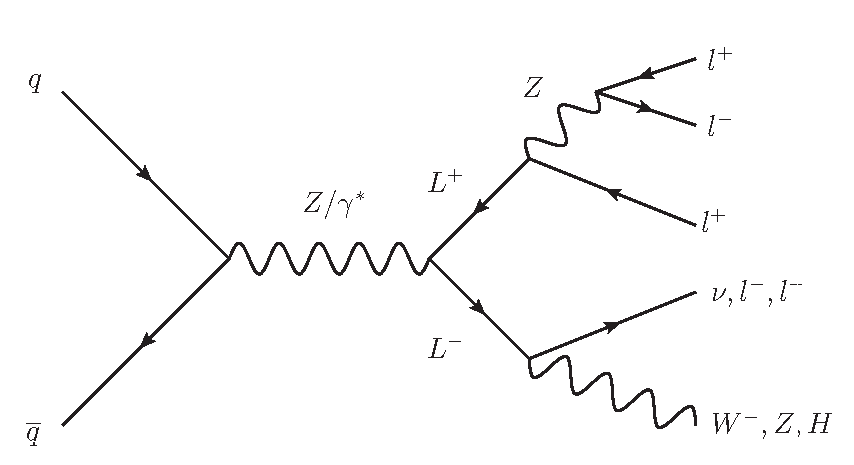
\includegraphics{figures/resonance/fd_cc2.eps}}
    \label{fig:heavy-lepton-feynman-diagrams-cc}
  }
  \subfloat[ Production of a charged and a neutral heavy lepton.] {
    \resizebox{0.45\textwidth}{!}{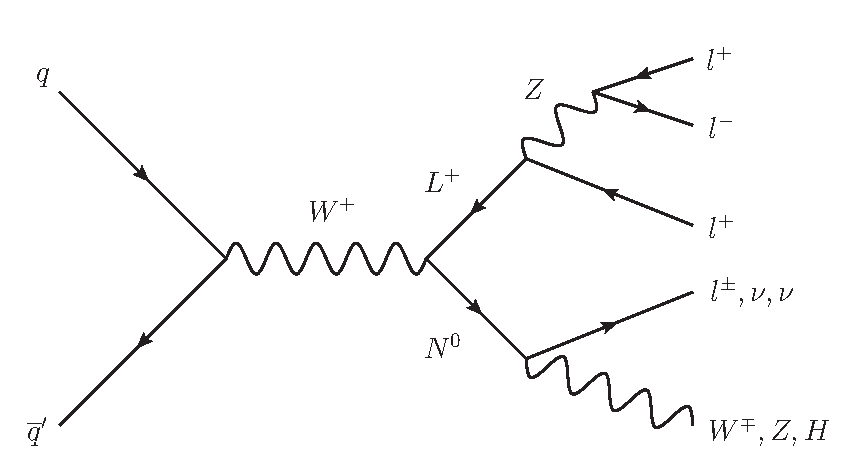
\includegraphics{figures/resonance/fd_cn2.eps}}
    \label{fig:heavy-lepton-feynman-diagrams-cn}
  }
  \caption{Production and decay of new heavy leptons to final states with a trilepton resonance.}
  \label{fig:heavy-lepton-feynman-diagrams}
\end{figure}

\begin{figure}[htbp]
	\centering
	\subfloat[ Type III Seesaw] {
		\resizebox{0.45\textwidth}{!}{\includegraphics{figures/resonance/c_xsec_t3ss.png}}
	}
	\hfill
	\subfloat[ Vector-Like Leptons] {
		\resizebox{0.45\textwidth}{!}{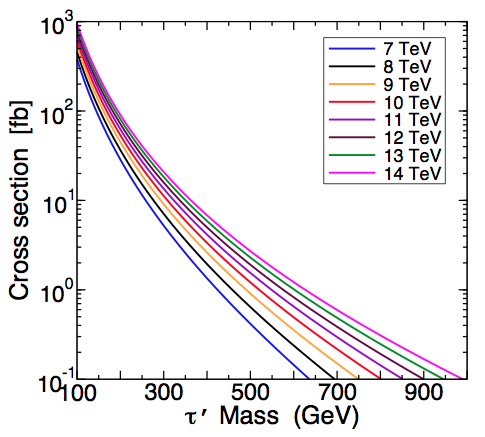
\includegraphics{figures/resonance/vll_xsec.png}}
	}
	\caption{Production cross sections at $\sqrt{s}=8 \TeV$ for heavy lepton pair production for the type~III seesaw model (left) and the vector-like leptons model (right).}
	\label{fig:resonance-production-cross-sections}
\end{figure}


The heavy leptons are made unstable by introducing mixing terms with the Standard Model leptons. For example, consider a single extra generation of fermions transforming in the adjoint representation of $\mathrm{SU}(2)_L$, as in the type~III seesaw model:

\begin{equation}
	\Sigma\equiv \left(\begin{array}{cc} \lzero/\sqrt{2} & \lplus \\ \lminus & -\lzero/\sqrt{2}\end{array}\right).
\end{equation}

The Lagrangian contains Yukawa terms mixing the heavy leptons with Standard Model leptons, $\ell=e,\,\mu,\,\tau$:
\begin{equation}
  -\mathcal{L} \ni \sum_{\ell=e,\,\mu,\,\tau} \sqrt{2}\phi^0 \overline{\Psi} Y_{L \ell} \psi_{\ell} + \mathrm{h.c.},
\end{equation}
where $\Psi\equiv {\lplus_R}^c + \lminus_R$ is a Dirac spinor representating the four charged degrees of freedom, $\psi_{\ell}$ are Dirac spinors corresponding to the Standard Model leptons, $\phi\equiv(\phi^+,\phi^0)^T\equiv (\phi^+,(v+H+i\eta)/\sqrt{2})^T$ is the Higgs doublet, and $Y_{L \ell}$ are Yukawa couplings. After electroweak symmetry breaking, the mass matrices take the form
\begin{equation}
-\mathcal{L} \ni \sum_{\ell=e,\mu,\tau} \left(\begin{array}{cc}\overline{\psi}_{\ell,R} & \overline{\Psi}_R \end{array} \right) \left(\begin{array}{cc} m_l & 0 \\ Y_{L \ell}v & M_{\lpm} \end{array}\right) \left(\begin{array}{c} \psi_{\ell,L} \\ \Psi_L \end{array}\right)  + \left(\begin{array}{cc}\overline{\psi}_{\ell,L} & \overline{\Psi}_L\end{array}\right) \left(\begin{array}{cc} m_l & Y_{L \ell}^{\dagger}v \\ 0 & M_{\lpm} \end{array}\right) \left(\begin{array}{c} \psi_{\ell,R} \\ \Psi_r \end{array}\right).
\end{equation}

Diagonalizing the mass matrices leads to off-diagonal terms in the gauge interactions, with couplings proportional to the mixing parameters $V_{L\ell}=\frac{v}{\sqrt{2}} M_{\lpm}^{-1} Y_{L \ell}$. These couplings enable the decay of the heavy leptons to a boson ($W$, $Z$, or $h$) plus a Standard Model lepton or neutrino, with partial widths given by:

%
\begin{align}
\label{eq:Gammatr0W}
\Gamma(\lzero \to \ell^- W^+) &=  \Gamma(\lzero \to \ell^+ W^-) =
\frac{g^2}{64 \pi} |V_{L\ell}|^2
\frac{M_{\lpm}^3}{M_W^2} \left( 1- \frac{M_W^2}{M_{\lpm}^2} \right)^2 
\left( 1 + 2 \frac{M_W^2}{M_{\lpm}^2} \right) , 
\\[0.1cm]
\label{eq:Gammatr0Z}
\sum_{\ell}\Gamma(\lzero \to \nu_{\ell} Z) &=  \frac{g^2}{64 \pi c_W^2} 
\sum_\ell |V_{L\ell}|^2
\frac{M_{\lpm}^3}{M_Z^2} \left( 1- \frac{M_Z^2}{M_{\lpm}^2} \right)^2 
\left( 1 + 2 \frac{M_Z^2}{M_{\lpm}^2}\right),
\\[0.2cm]
\label{eq:Gammatr0h}
\sum_{\ell}\Gamma(\lzero \to \nu_{\ell} H) &=  \frac{g^2}{64 \pi} 
\sum_\ell |V_{L\ell}|^2
\frac{M_{\lpm}^3}{M_W^2} \left( 1- \frac{M_H^2}{M_{\lpm}^2} \right)^2 ,
\\[0.2cm]
\label{eq:Gammatr+W}
\sum_{\ell}\Gamma(\lplus \to \nu_{\ell} W^+) &= 
\frac{g^2}{32 \pi} \sum_\ell |V_{L\ell}|^2
\frac{M_{\lpm}^3}{M_W^2} \left( 1- \frac{M_W^2}{M_{\lpm}^2} \right)^2 
\left( 1 + 2 \frac{M_W^2}{M_{\lpm}^2} \right) ,
\\[0.2cm]
\label{eq:Gammatr+Z}
\Gamma(\lplus \to \ell^+ Z) &= 
\frac{g^2}{64 \pi c_W^2} |V_{L\ell}|^2
\frac{M_{\lpm}^3}{M_Z^2} \left( 1- \frac{M_Z^2}{M_{\lpm}^2} \right)^2 
\left( 1 + 2 \frac{M_Z^2}{M_{\lpm}^2}\right),
\\[0.2cm]
\label{eq:Gammatr+h}
\Gamma(\lplus \to \ell^+ H) &= \frac{g^2}{64 \pi} |V_{L\ell}|^2
\frac{M_{\lpm}^3}{M_W^2} \left( 1- \frac{M_H^2}{M_{\lpm}^2} \right)^2 .
\end{align}

The branching fractions of the charged and neutrino heavy leptons are shown as function of $m_{\lpm}$ in figure~\ref{fig:resonance-branching-ratios}. Note that these branching fractions are common to all the models considered in this analysis (aside from the possibility of only having a charged heavy lepton).


\begin{figure}[h]
  \centering
  \subfloat[ Charged heavy fermion] {
    \resizebox{0.45\textwidth}{!}{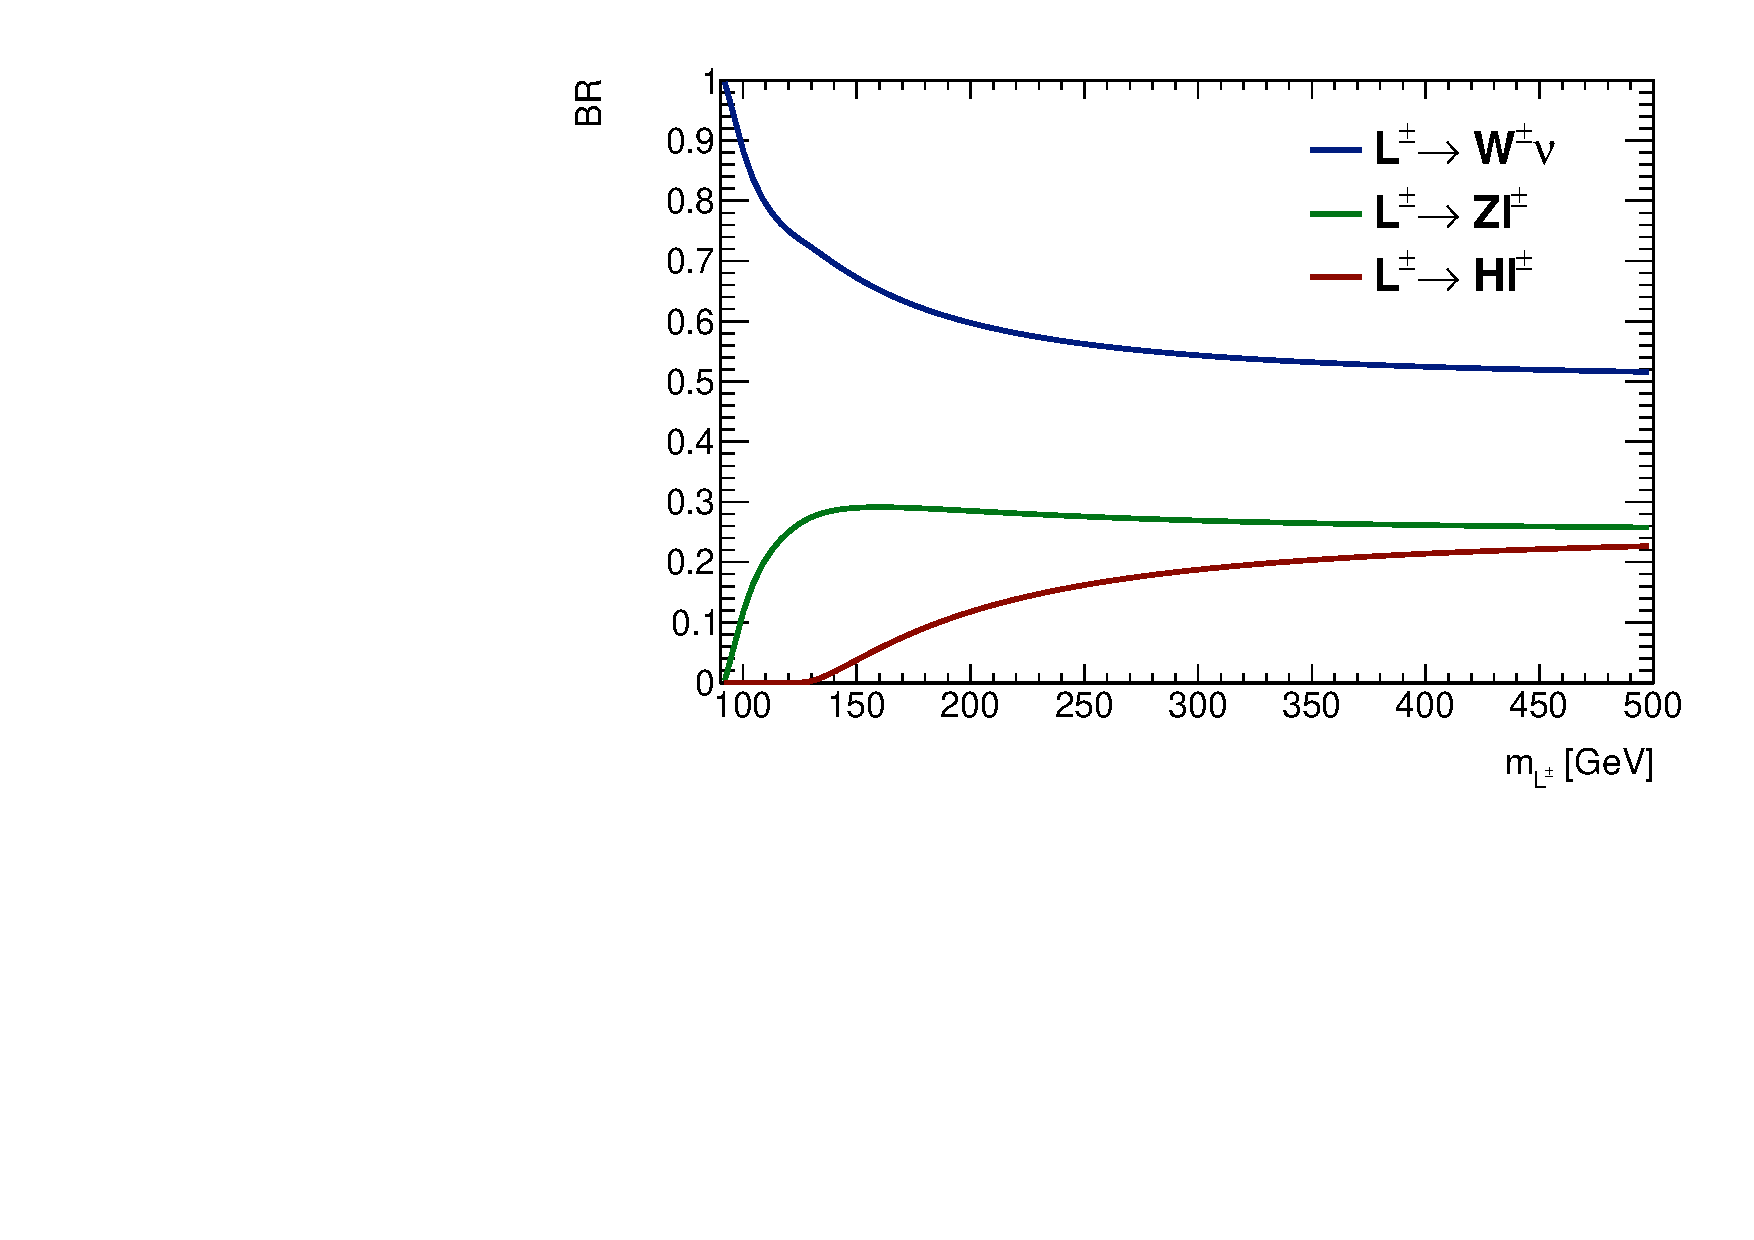
\includegraphics{figures/resonance/c_br_charged}}
  }
  \subfloat[ Neutral heavy fermion] {
    \resizebox{0.45\textwidth}{!}{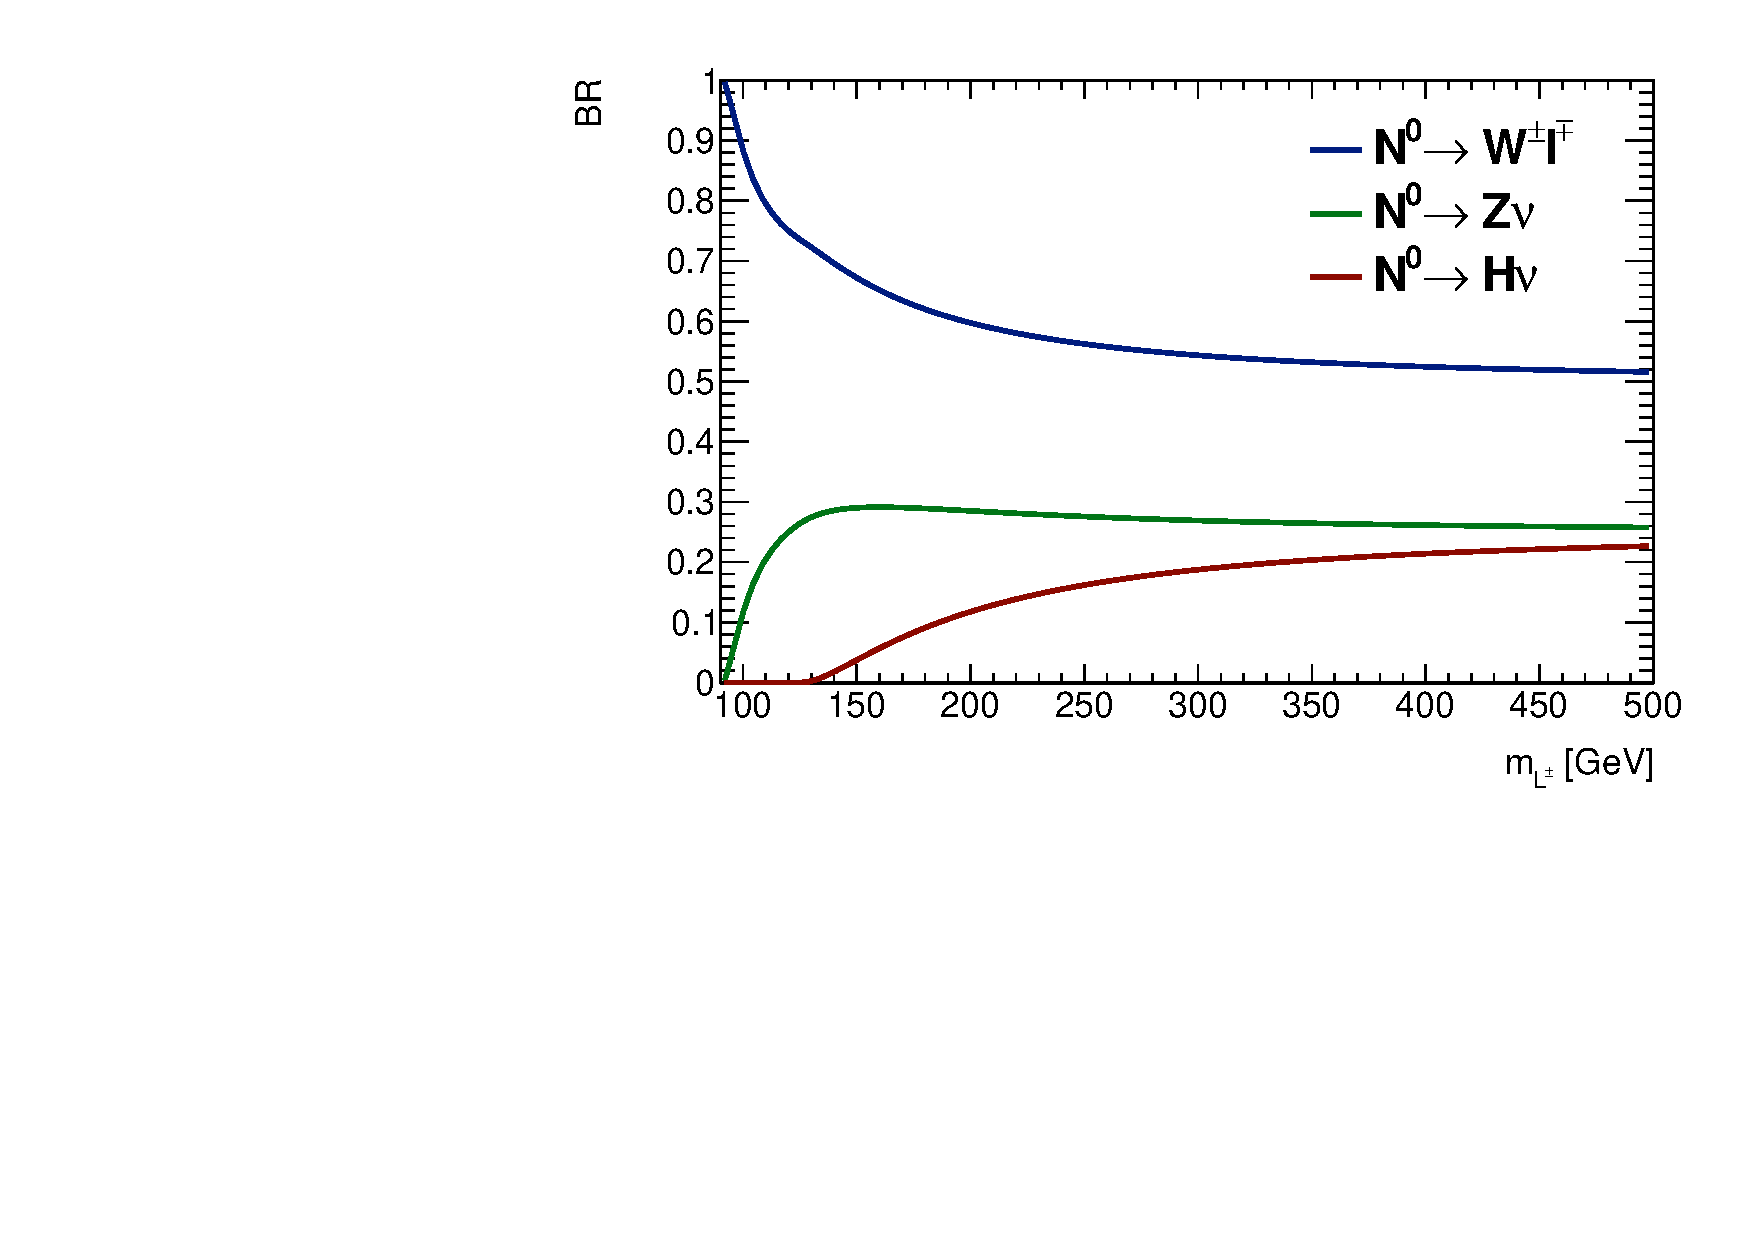
\includegraphics{figures/resonance/c_br_neutral}}
  }
  \caption{Branching ratios of a heavy lepton decaying via mixing with Standard Model leptons.}
  \label{fig:resonance-branching-ratios}
\end{figure}

Constraints on the mixing parameters $V_{L\ell}$ can be derived from precision measurements of the $Z$ width, and constraints on products of the mixing parameters from flavor violation experiments like $\mu\rightarrow e\gamma$~\cite{Abada:2008hr,Abada:2007kn,delAguila:2008cv,Altmannshofer:2014ej}:

\begin{align}
|V_{L e}| & <5.5\times10^{-2}\\
|V_{L \mu}| & <6.3\times10^{-2}\\
|V_{L \tau}| & <6.3\times10^{-2}\\
|V_{L e}V_{L\mu}| & <1.7\times10^{-7}\\
|V_{L e}V_{L\tau}| & <4.2\times10^{-4}\\
|V_{L \mu}V_{L\tau}| & <4.9\times10^{-4}.
\end{align}

\subsection{Signal Monte Carlo Samples}\label{sec:resonance-signal-mc-samples}

Signal events are generated using Monte Carlo simulation, with eleven mass hypotheses in the range $100 \GeV \leq m_{\lpm} \leq 400 \GeV$ for the vector-like leptons model and ten mass hypothesis in the range $100 \GeV \leq m_{\lpm,\lzero}\leq 500 \GeV$ for the type~III seesaw model. The samples are summarized in table~\ref{table:resonance-signal-samples}. The events are generated with \madgraph~4.5.2 and 5.2.2.1~\cite{madgraph}, for the vector-like leptons and type~III seesaw models, respectively, using the CTEQ6L1~\cite{ct6l1} PDF set and the AU2 underlying event tune~\cite{AU2}. Showering is performed with \pythia\ 8~\cite{Sjostrand:2008bk}. Decays of the heavy leptons in the vector-like leptons model are performed using \bridge~\cite{bridge}, while decays in the type~III seesaw samples are performed by \madgraph. The cross sections for both samples are calculated at leading order (LO) in QCD, and are shown in table~\ref{table:resonance-signal-samples}. 

For the type~III seesaw model, the charged and neutral heavy leptons are generated with identical masses. The simulated decay modes are listed in table~\ref{table:resonance-seesaw-sample-decays}. The mixing parameters are chosen to be $V_{L e}=0.055$, $V_{L\mu}=0.063$, and $V_{L\tau}=0$, yielding a mix of $ee$, $e\mu$, and $\mu\mu$ decays. For the vector-like leptons model, one heavy lepton is required to decay via $L^{\pm}\rightarrow Z(\ell\ell)\ell$, where $\ell=e,\mu,\tau$. The two heavy leptons are constrained to decay to the same flavor of Standard Model lepton, which is chosen with equal probability to be an electron, muon, or tau. For both models, the events are divided and reweighted to correspond to electron-only or muon-only mixing scenarios. 

The type~III seesaw samples were simulated with no intrinsic width for the $Z$ bosons. As a result, the signal peaks are slightly narrower than would be expected if the $Z$ width were correctly included. As described below in section~\ref{sec:resonance-signal-model}, the limit setting is performed by fitting the trilepton mass distributions with analytical functions. In order to incorporate the missing $Z$ width into the signal peaks, the peak width parameters determined from the vector-like lepton samples are used for the type~III seesaw model. 


\begin{table}[htbp]
	\centering
	\resizebox{\textwidth}{!}{
		\begin{tabular}{|l||c|c|c|r|}
			\hline
			Mass [GeV]  & Cross Section [pb] & Filter Efficiency & Number of Events \\
			\hline
			\multicolumn{5}{|c|}{Type III Seesaw} \\
			\hline
			100	&	1.273		&	0.1018	&	100,000 \\
			\hline
			120	&	2.138		&	0.1628	&	100,000 \\
			\hline
			160	&	0.853		&	0.1808	&	100,000 \\
			\hline
			200	&	0.346		&	0.2012	&	100,000 \\
			\hline
			250	&	0.135		&	0.2096	&	100,000 \\
			\hline
			300	&	0.0604		&	0.2178	&	50,000 	\\
			\hline
			350	&	0.02969		&	0.2337	&	50,000 	\\
			\hline
			400	&	0.01566		&	0.2409	&	50,000 	\\
			\hline
			450	&	0.008733	&	0.2456	&	50,000 	\\
			\hline
			500	&	0.00504		&	0.2493	&	50,000 	\\
			\hline
			\hline
			\multicolumn{5}{|c|}{Vector-Like Leptons} \\
			\hline
			100	&	0.378 	&	0.0233	& 100,000 \\
			\hline
			110	&	0.264 	&	0.0412	& 100,000 \\
			\hline
			120	&	0.193 	&	0.0498	& 100,000 \\
			\hline
			130	&	0.142 	&	0.0548	& 100,000 \\
			\hline
			140	&	0.106 	&	0.0569	& 100,000 \\
			\hline
			160	&	0.0645 	&	0.0579	& 100,000 \\
			\hline
			180	&	0.0407 	&	0.0575	& 100,000 \\
			\hline
			200	&	0.0265 	&	0.0567	& 100,000 \\
			\hline
			250	&	0.0104 	&	0.0548	& 100,000 \\
			\hline
			300	&	0.00457	&	0.0536	& 100,000 \\
			\hline
			400	&	0.00115	&	0.0520	& 100,000 \\
			\hline
		\end{tabular}
	}
	\caption{Summary of signal Monte Carlo samples. Ten mass points are simulated for the type~III seesaw model, and eleven for the vector-like leptons model.}
	\label{table:resonance-signal-samples}
\end{table}

\begin{table}
	\centering
	\begin{tabular}{c|ll}
		Production Mode & Decay 1 & Decay 2 \\
		\hline
		$pp \rightarrow \lzero\lplus$	&	$\lzero \rightarrow \ell^{+} W^{-}$	&	$\lplus \rightarrow \ell^{+} Z$ \\
		$pp \rightarrow \lzero\lplus$	&	$\lzero \rightarrow \ell^{-} W^{+}$	&	$\lplus \rightarrow \ell^{+} Z$ \\
		$pp \rightarrow \lzero\lplus$	&	$\lzero \rightarrow \nu_{\ell} Z$		&	$\lplus \rightarrow \ell^{+} Z$ \\
		$pp \rightarrow \lzero\lplus$	&	$\lzero \rightarrow \nu_{\ell} H$		&	$\lplus \rightarrow \ell^{+} Z$ \\
		$pp \rightarrow \lzero\lminus$	&	$\lzero \rightarrow \ell^{-} W^{+}$	&	$\lminus \rightarrow \ell^{-} Z$ \\
		$pp \rightarrow \lzero\lminus$	&	$\lzero \rightarrow \ell^{+} W^{-}$	&	$\lminus \rightarrow \ell^{-} Z$ \\
		$pp \rightarrow \lzero\lminus$	&	$\lzero \rightarrow \nu_{\ell} Z$		&	$\lminus \rightarrow \ell^{-} Z$ \\
		$pp \rightarrow \lzero\lminus$	&	$\lzero \rightarrow \nu_{\ell} H$		&	$\lminus \rightarrow \ell^{-} Z$ \\
		$pp \rightarrow \lminus\lplus$	&	$\lminus \rightarrow \ell^{-} Z$		&	$\lplus \rightarrow \ell^{+} Z$ \\
		$pp \rightarrow \lminus\lplus$	&	$\lminus \rightarrow \nu_{l} W^{-}$	&	$\lplus \rightarrow \ell^{+} Z$ \\
		$pp \rightarrow \lminus\lplus$	&	$\lminus \rightarrow \ell^{-} H$		&	$\lplus \rightarrow \ell^{+} Z$ \\
		$pp \rightarrow \lminus\lplus$	&	$\lminus \rightarrow \ell^{-} Z$		&	$\lplus \rightarrow \nu_{l} W^{+}$ \\
		$pp \rightarrow \lminus\lplus$	&	$\lminus \rightarrow \ell^{-} Z$		&	$\lplus \rightarrow \ell^{+} H$ \\
	\end{tabular}
	\caption{Decays simulated for the type~III seesaw signal samples.}
	\label{table:resonance-seesaw-sample-decays}
\end{table}



\section{Search Strategy}\label{sec:resonance-search-strategy}
\subsection{Event Selection and Heavy Lepton Reconstruction}\label{sec:event-3l-selection}
The event selection is very similar to that used in the model-independent analysis, described in section~\ref{sec:model-independent-event-selection}. In particular, the same definitions are used for leptons and jets, in order to make use of the same fake factor method to estimate the reducible backgrounds. Events containing a heavy lepton candidate are selected as follows.

\begin{itemize}
	\item Events are triggered using the lowest-threshold unprescaled single-electron and single-muon triggers, \texttt{EF\_e24vhi\_medium1}, \texttt{EF\_e60\_medium1}, \texttt{EF\_mu24i\_tight}, and \texttt{EF\_mu36\_tight} (section~\ref{sec:model-independent-event-selection-triggering}).
	\item The primary event vertex must have at least three tracks with $\pt>400~\mbox{MeV}$.
	\item Events are required to have at least three electrons or muons ($eee$, $ee\mu$, $\mu\mu e$, $\mu\mu\mu$) satisfying the lepton selection criteria (table~\ref{table:electron-muon-selections}). 
	\item Events must have one $Z$ candidate, consisting of a same-flavor, opposite-sign pair of leptons with $|m_{l^+l^-}-m_{Z}|<10~\mbox{GeV}$. The $Z$ mass is taken to be $m_Z=91.1876~\mbox{GeV}$~\cite{pdg}. 
	\item Four-lepton events with two leptonic $Z$ candidates with $|m_{\ell\ell}-m_Z|<\SI{10}{\giga\electronvolt}$ are rejected to suppress the Standard Model $ZZ$ background. The efficiency loss for signal events is low; see tables~\ref{table:fiducial-efficiencies-Ze} and \ref{table:fiducial-efficiencies-Zmu}. 
	\item If an event contains more than three leptons, a unique trilepton candidate in each event is chosen as follows:
	\begin{itemize}
		\item Choose the same-flavor, opposite-sign pair with invariant mass closest to $m_{Z}$.
		\item Choose the third (``off-$Z$'') lepton to be the closest in $\Delta R$ to the reconstructed $Z$ four-momentum.
	\end{itemize}
	\item For low heavy lepton mass hypotheses, $m_{\lpm}\lesssim 200~\mbox{GeV}$, the $Z$ and the third lepton will tend to be collimated. The expected background and signal $\Delta R$ distributions for selected trilepton candidate are shown in figure~\ref{fig:resonance-inclusive-dR}. Imposing a cut on the $\Delta R(Z,\,\ell_3)$ of the trilepton candidates improves the signal significance, and also provides a useful control region defined by inverting the cut. The value of the cut is chosen by comparing the expected sensitivities of the analysis with different cuts values, described in appendix~\ref{sec:appendix-resonance-dr-optimization}. A flat cut of $\Delta R(Z,\,\ell_3)<3.0$ is used, independent of the heavy lepton mass hypothesis. 

	\begin{figure}[h]
		\centering
		\resizebox{0.6\textwidth}{!}{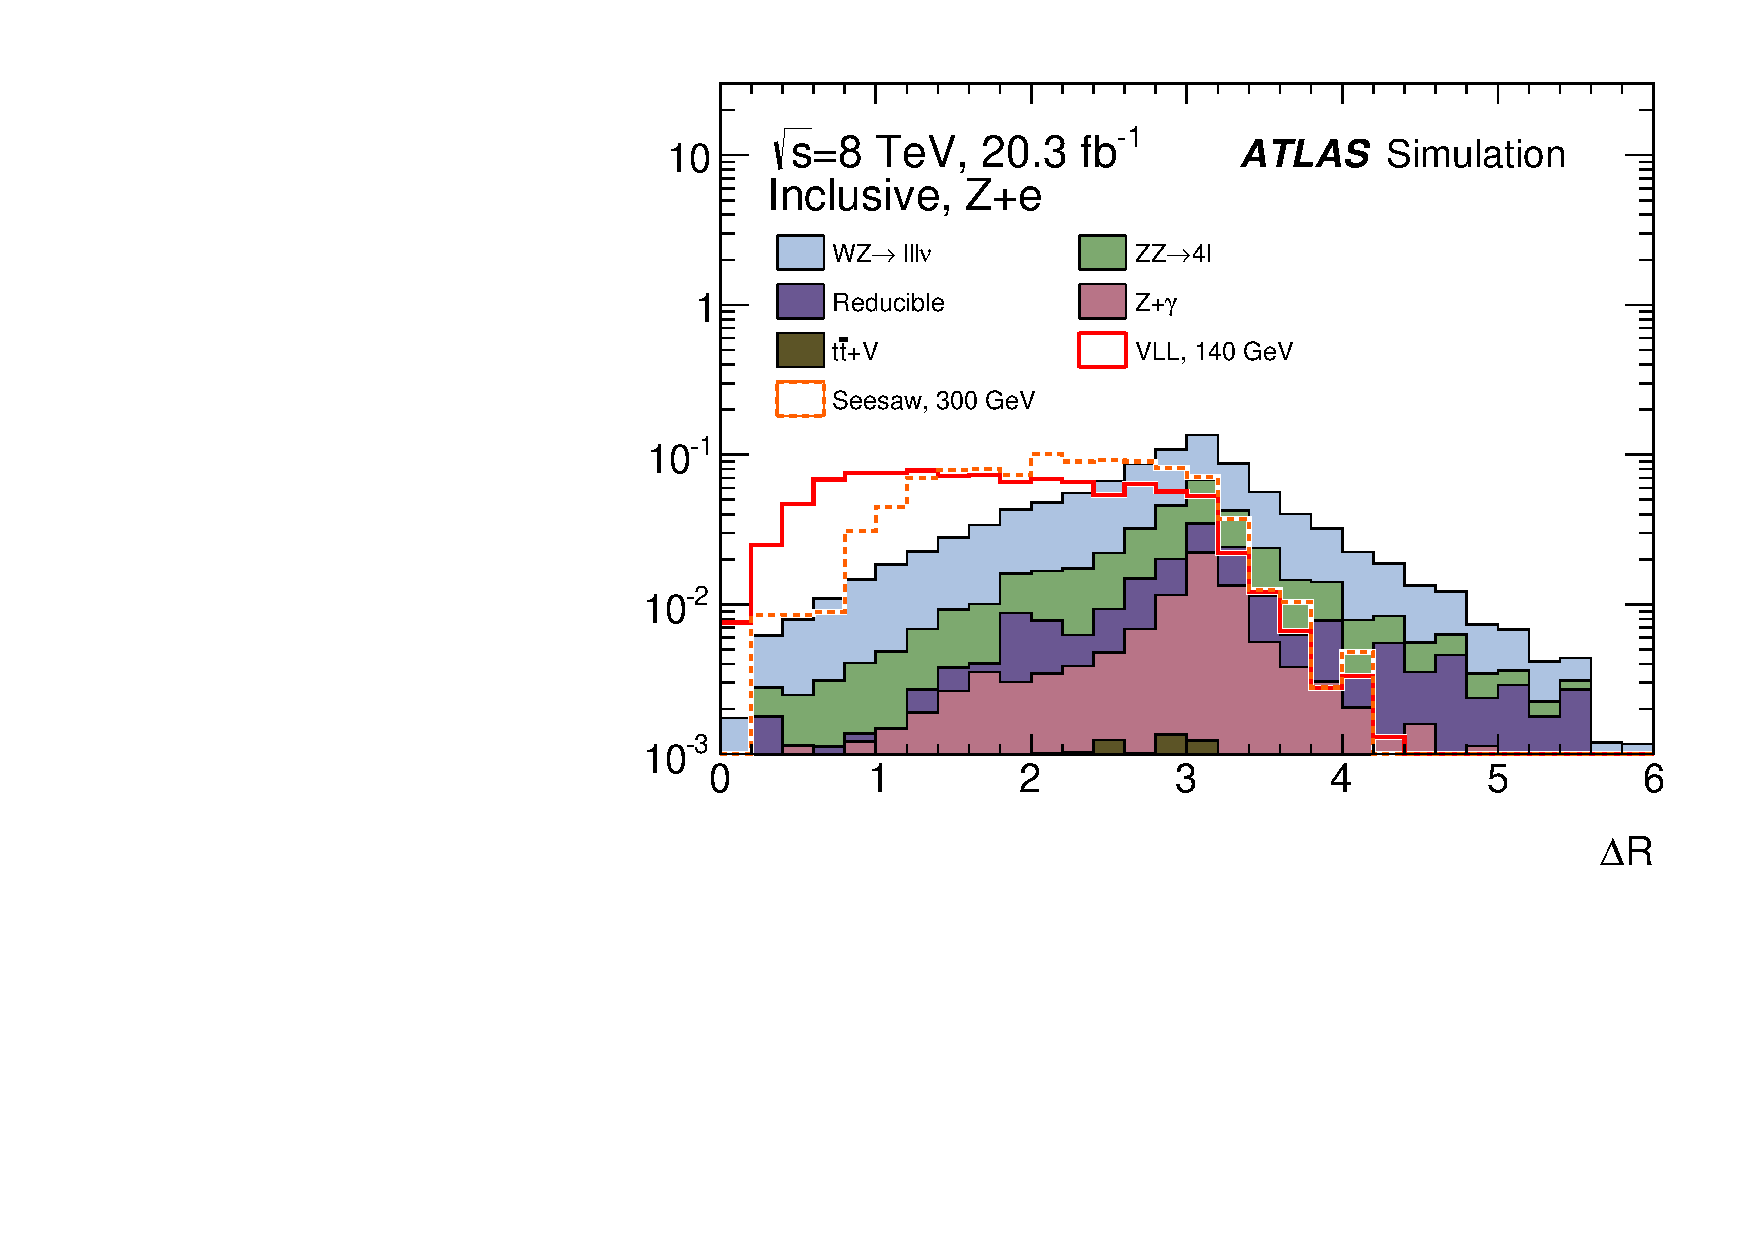
\includegraphics{figures/resonance/c_output_dR_Ze_InclusiveNoM3LDeltaR_300GeV_log_blind_hide_ratio_force_draw_signal}}
		\caption{Expected $\Delta R(Z,\,\ell_3)$ distributions for background and signal in the inclusive signal region.}
		\label{fig:resonance-inclusive-dR}
	\end{figure}
  
	\item The variable of interested used to apply the trilepton mass constraint is $\Delta m \equiv m_{3\ell}-m_{\ell^+\ell^-}$, where the invariant mass of the two leptons associated with a $Z$ boson decay is subtracted by the trilepton mass. This method reduces the impact of the lepton energy or momentum resolutions on the width of the resonance peak, at the cost of introducing some width due to the intrinsic width of the $Z$, $\Gamma_Z=2.4952\pm0.0023 \GeV$~\cite{pdg}. Over most of the mass range, this variable reduces the width of the signal peaks, as shown in figure~\ref{fig:deltam-m3l-comparison}. 

	\begin{figure}[htbp]
		\textcolor{red}{m3l deltam comparison plot or table}
		\caption{Comparison of the full-width, half-maximum of the signal peaks between the $\deltam$ and $m_{3\ell}$ variables.}
		\label{fig:deltam-m3l-comparison}
	\end{figure}
	  
\end{itemize}

After identifying the trilepton candidates, six mutually exclusive signal regions are defined. First, to target the flavor structure of the heavy lepton mixing, events are divided into two flavor channels, $Z+e$ and $Z+\mu$, depending on the flavor the off-$Z$ lepton. Second, as the heavy leptons are pair produced, signal events will contain additional activity due to the decay of the second heavy lepton. Events are divided into three exclusive categories based on other activity in the event:
  \begin{itemize}
  	\item \textbf{\fourl}: events containing a fourth lepton, either an electron or a muon, passing the normal lepton criteria. 
  	\item \textbf{\threeljj}: events containing exactly three leptons and a dijet with $60.385~\mbox{GeV}<m_{jj}<150.9~\mbox{GeV}$. 
  	\item \textbf{\threelo}: all other events, i.e. events with three leptons and no jet pair satisying the invariant mass requirement. 
  \end{itemize}

 The choice of these three categories is motivated in figure~\ref{fig:opposite-side-br}, which shows the fraction of events with various activity from the decay of the other heavy lepton. The additional activity includes extra leptons and neutrinos, and jets from $W/Z/h$ decays. Assuming that the mixing with tau leptons is zero ($V_{\tau L}=0$), the requirements of a fourth lepton or a hadronically decaying boson are very efficient on signal. If the second heavy fermion is charged, then the only decay mode that fails both requirements is $\lpm\rightarrow W^{\pm}(\tau^{\pm}\nu)\nu$. If the second heavy fermion is neutral, then only the $\lzero\rightarrow Z(\nu\nu)\nu$ and a small fraction of $\lzero \rightarrow H\nu$ decays fail both requirements. Categorization targeting neutrinos is less effective at separating signal from the large $WZ$ background (see figures~\ref{fig:SR-mTW-1}-\ref{fig:SR-ETMiss-2}). 

In some cases, it is useful to consider the events without dividing into these three categories, distinguishing events only by the flavor of the off-$Z$ lepton. This is referred to as the ``Inclusive'' signal region below.

\begin{figure}
	\subfloat[ $\lpm$] {
		\resizebox{0.48\textwidth}{!}{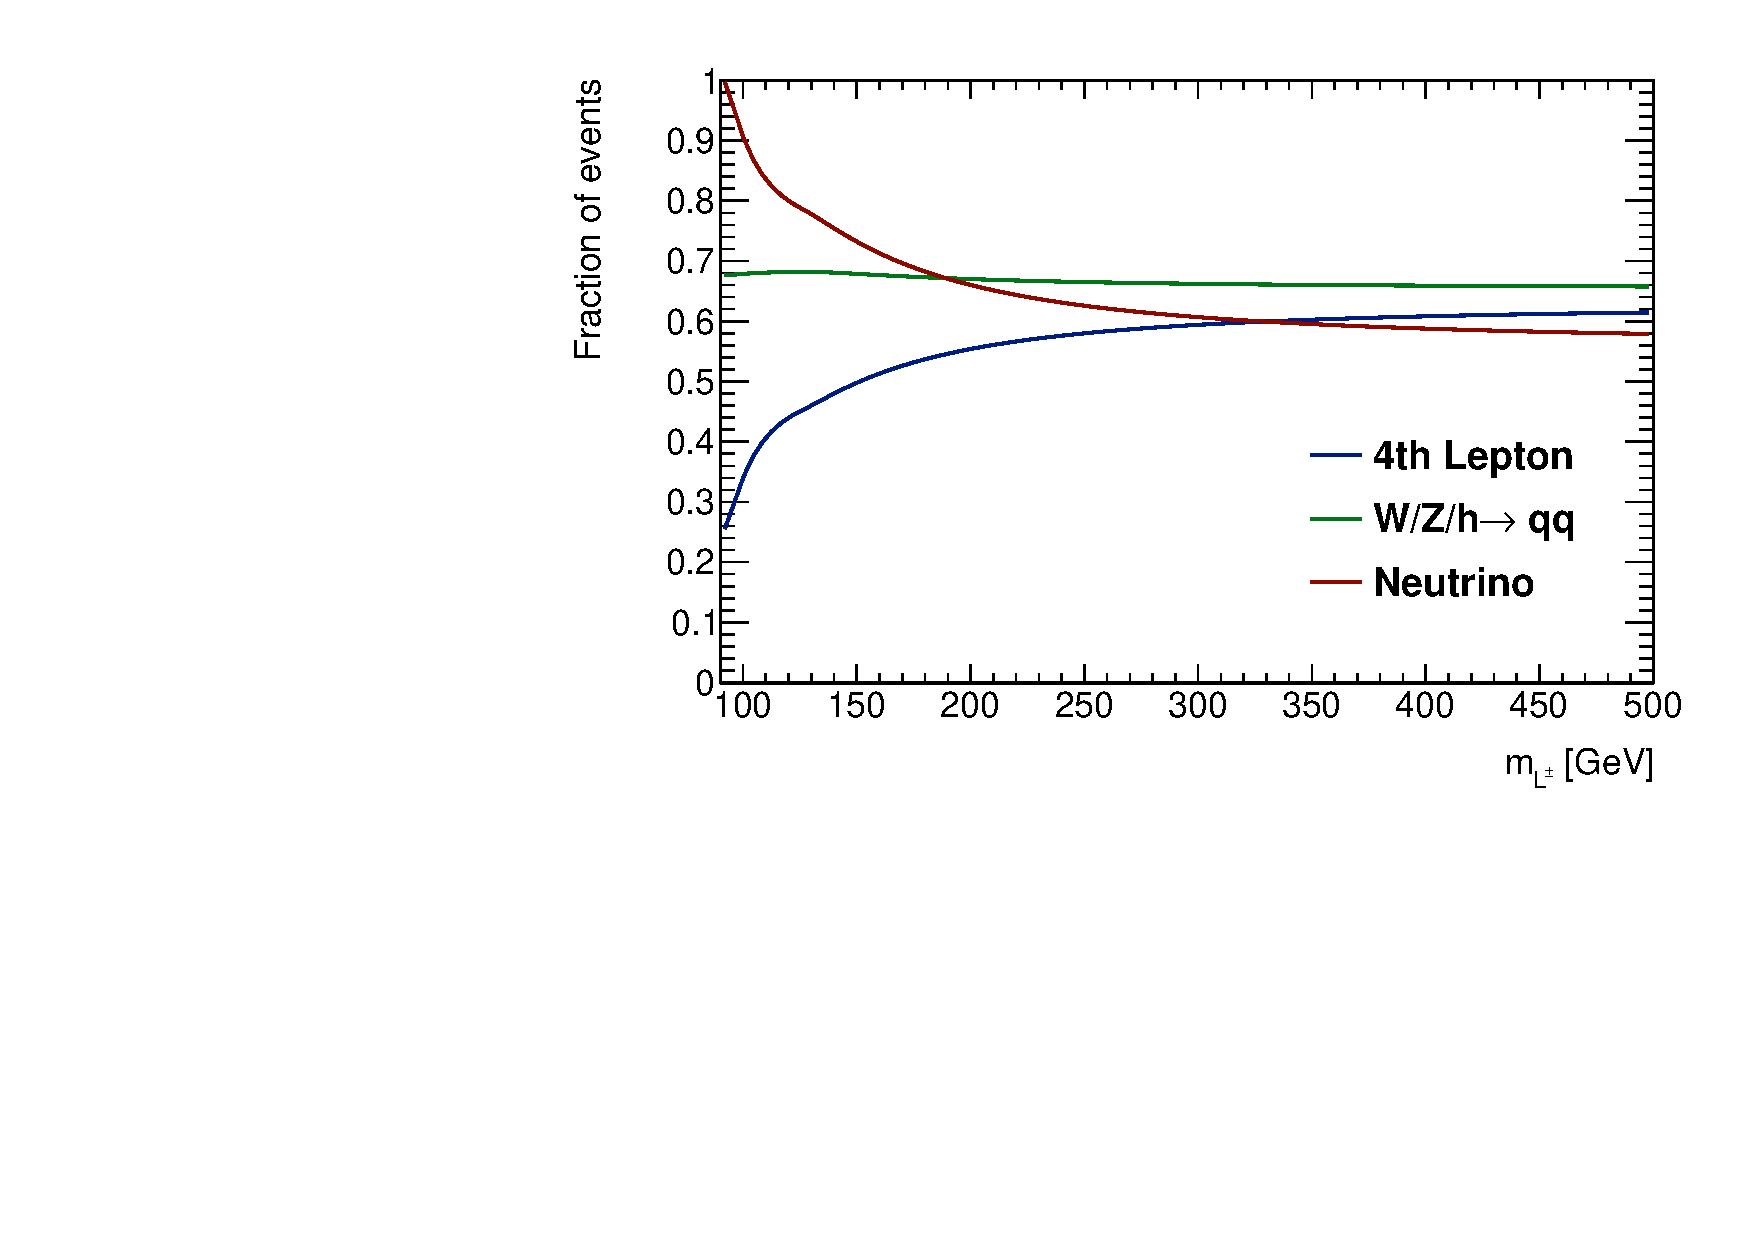
\includegraphics{figures/resonance/c_oppositesideactivity_charged.pdf}}
	}
	\subfloat[ $\lzero$] {
		\resizebox{0.48\textwidth}{!}{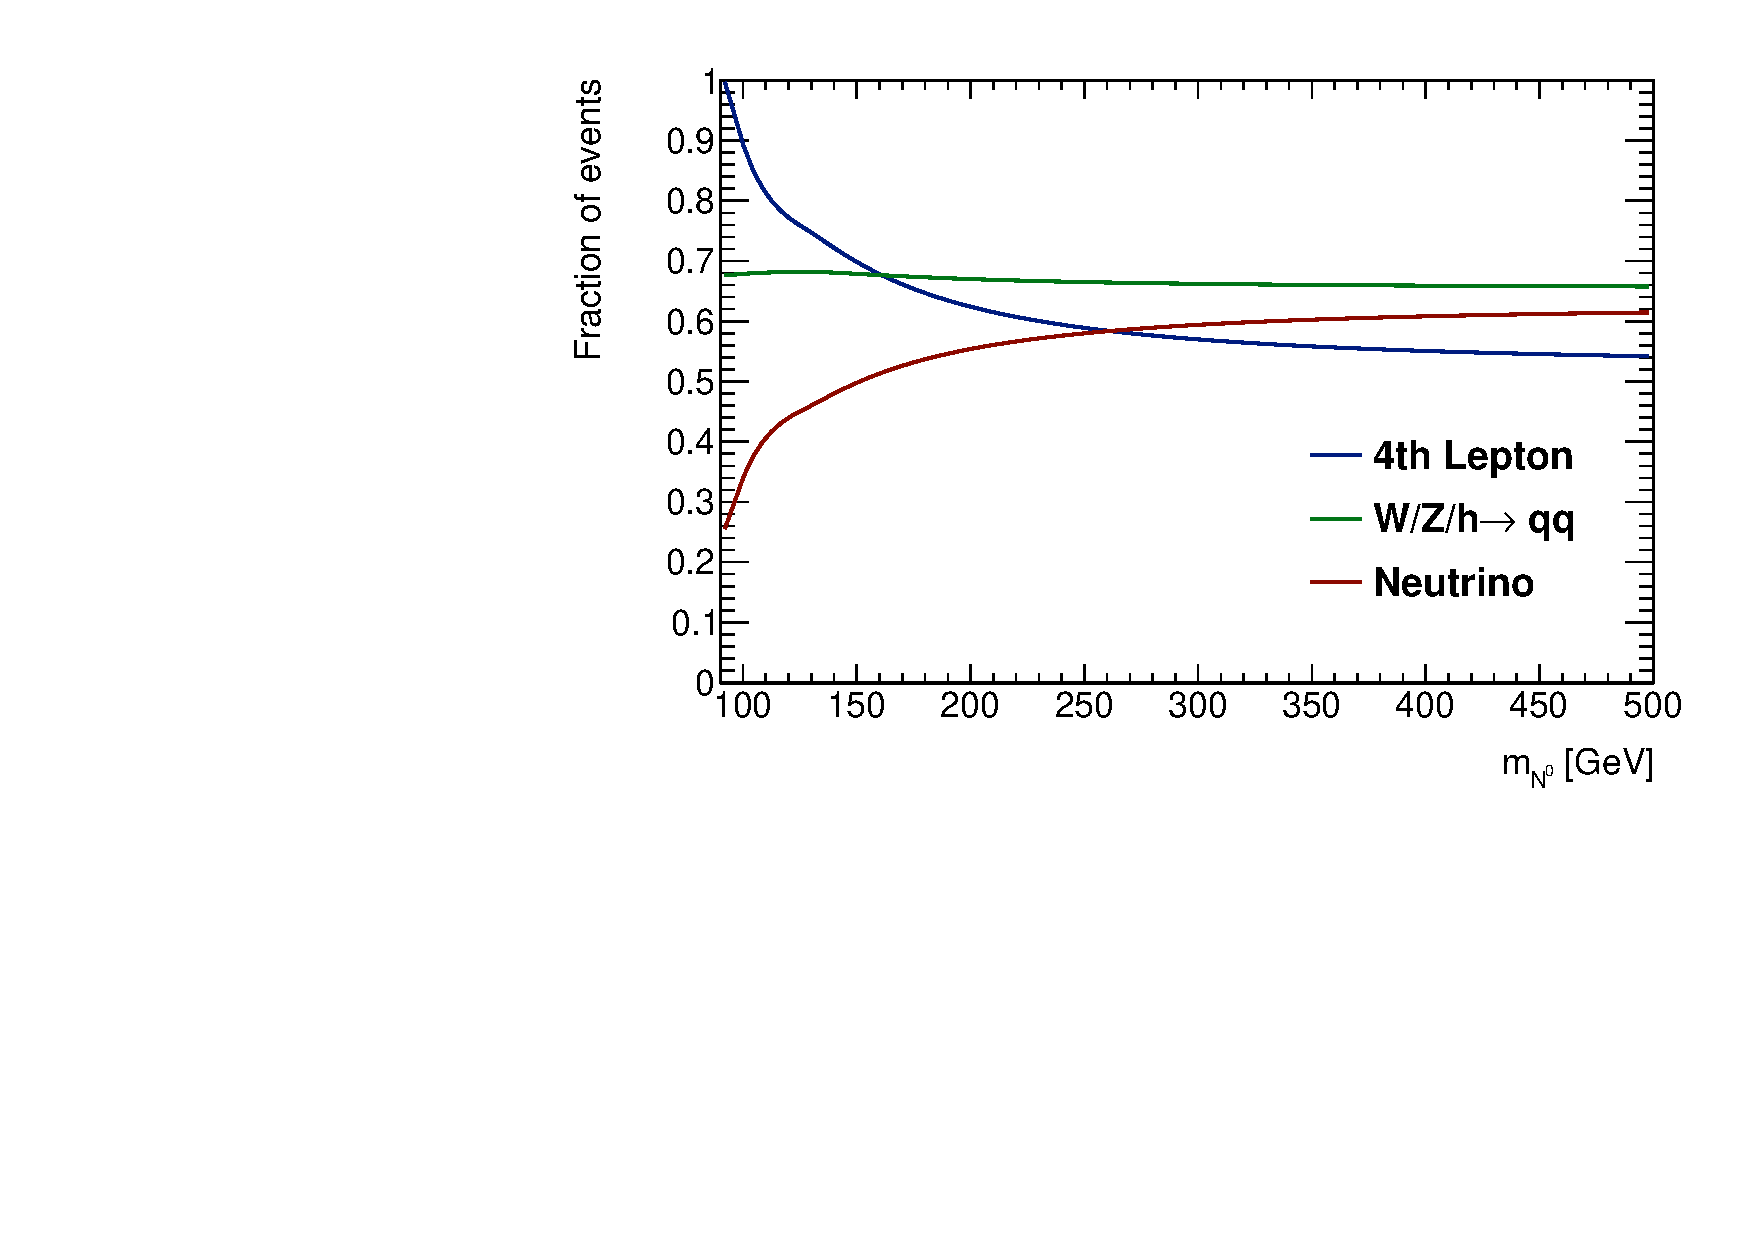
\includegraphics{figures/resonance/c_oppositesideactivity_neutral.pdf}}
	}
	\caption{Fraction of events with various activity on the opposite side of the event, for $\lpm\lmp$ events at left, and $\lpm\lzero$ events at right. The left plot, showing the opposite side activity for a $\lpm\lmp$ final state, is identical for the seesaw and vector-like lepton model.
	}
	\label{fig:opposite-side-br}
\end{figure}

\subsection{Performance on Fiducial Signal Events}\label{sec:fiducial-cutflow}
The performance of the cuts and heavy lepton candidate selection is shown in tables~\ref{table:fiducial-efficiencies-Ze} and \ref{table:fiducial-efficiencies-Zmu} in terms of efficiency on fiducial events. The fiducial selection requires the event to have three truth-level leptons satisfying $\pt>15~\mbox{GeV}$ and $|\eta|<2.5$, of which two form a $Z$ candidate with $|m_{\ell^+ \ell^-}-m_Z|<10~\mbox{GeV}$, the third lepton is of the correct flavor, and the trilepton mass satisfies $|m_{3\ell}-m_{\lpm}|<5~\mbox{GeV}$. The final efficiency to reconstruct and select fiducial events for each signal region is shown as a function of signal mass $m_{\lpm}$ in figure~\ref{fig:fiducial-efficiencies-vs-mass}.

Note that cut imposing a flavor requirement on the reconstructed off-$Z$ lepton has a different efficiency between the vector-like lepton sample and the seesaw sample. This is a consequence of the initial flavor content of the samples: the vector-like lepton samples are divided into two samples with with 100\% branching fraction to either bachelor electron or bachelor muon, while the seesaw samples is a single mixed sample containing both electron and muon decays. 


\begin{table}[ht]
	\resizebox{\textwidth}{!}{
	\begin{tabular}{|c|c|c|c|c|c||c|c|c|}
		\hline
		Process  & Preselection  & Bachelor $e$  & $|m_{\ell^{+}\ell^{-}} - m_{Z}|<10~\mbox{GeV}$  & !$2Z$  & $\Delta R < 3.0$  & $\fourl$ & $\threeljj$ & $\threelo$ \\
		\hline
		VLL, $100$~GeV		&	$0.348 \pm 0.008$	&	$0.318 \pm 0.008$	&	$0.306 \pm 0.008$	&	$0.303 \pm 0.008$	&	$0.298 \pm 0.008$	&	$0.054 \pm 0.004$ &	$0.096 \pm 0.005$	&	$0.147 \pm 0.006$	\\
		\hline
		VLL, $110$~GeV		&	$0.478 \pm 0.006$	&	$0.435 \pm 0.006$	&	$0.421 \pm 0.006$	&	$0.417 \pm 0.006$	&	$0.401 \pm 0.006$	&	$0.076 \pm 0.003$ &	$0.11 \pm 0.004$	&	$0.215 \pm 0.005$	\\
		\hline
		VLL, $120$~GeV		&	$0.535 \pm 0.006$	&	$0.491 \pm 0.006$	&	$0.467 \pm 0.006$	&	$0.457 \pm 0.006$	&	$0.424 \pm 0.006$	&	$0.104 \pm 0.004$ &	$0.117 \pm 0.004$	&	$0.204 \pm 0.005$	\\
		\hline
		VLL, $130$~GeV		&	$0.604 \pm 0.006$	&	$0.539 \pm 0.006$	&	$0.509 \pm 0.006$	&	$0.494 \pm 0.006$	&	$0.445 \pm 0.006$	&	$0.125 \pm 0.004$ &	$0.127 \pm 0.004$	&	$0.194 \pm 0.005$	\\
		\hline
		VLL, $140$~GeV		&	$0.643 \pm 0.006$	&	$0.578 \pm 0.006$	&	$0.559 \pm 0.006$	&	$0.538 \pm 0.006$	&	$0.491 \pm 0.006$	&	$0.153 \pm 0.004$ &	$0.164 \pm 0.004$	&	$0.174 \pm 0.005$	\\
		\hline
		VLL, $160$~GeV		&	$0.663 \pm 0.006$	&	$0.593 \pm 0.006$	&	$0.572 \pm 0.006$	&	$0.552 \pm 0.006$	&	$0.499 \pm 0.006$	&	$0.175 \pm 0.005$ &	$0.148 \pm 0.004$	&	$0.176 \pm 0.005$	\\
		\hline
		VLL, $180$~GeV		&	$0.698 \pm 0.006$	&	$0.62 \pm 0.006$	&	$0.594 \pm 0.006$	&	$0.573 \pm 0.007$	&	$0.505 \pm 0.007$	&	$0.197 \pm 0.005$ &	$0.163 \pm 0.005$	&	$0.144 \pm 0.005$	\\
		\hline
		VLL, $200$~GeV		&	$0.707 \pm 0.006$	&	$0.624 \pm 0.007$	&	$0.596 \pm 0.007$	&	$0.577 \pm 0.007$	&	$0.52 \pm 0.007$	&	$0.209 \pm 0.006$ &	$0.167 \pm 0.005$	&	$0.145 \pm 0.005$	\\
		\hline
		VLL, $250$~GeV		&	$0.751 \pm 0.007$	&	$0.654 \pm 0.007$	&	$0.626 \pm 0.007$	&	$0.615 \pm 0.007$	&	$0.548 \pm 0.008$	&	$0.245 \pm 0.007$ &	$0.152 \pm 0.005$	&	$0.151 \pm 0.005$	\\
		\hline
		VLL, $300$~GeV		&	$0.771 \pm 0.007$	&	$0.662 \pm 0.008$	&	$0.63 \pm 0.008$	&	$0.625 \pm 0.008$	&	$0.547 \pm 0.008$	&	$0.258 \pm 0.007$ &	$0.169 \pm 0.006$	&	$0.121 \pm 0.005$	\\
		\hline
		VLL, $400$~GeV		&	$0.776 \pm 0.007$	&	$0.669 \pm 0.008$	&	$0.642 \pm 0.008$	&	$0.641 \pm 0.008$	&	$0.562 \pm 0.008$	&	$0.277 \pm 0.007$ &	$0.181 \pm 0.006$	&	$0.103 \pm 0.005$	\\
		\hline
		Seesaw, $100$~GeV	&	$0.381 \pm 0.006$	&	$0.351 \pm 0.005$	&	$0.336 \pm 0.005$	&	$0.334 \pm 0.005$	&	$0.308 \pm 0.005$	&	$0.08 \pm 0.003$ &	$0.096 \pm 0.003$	&	$0.131 \pm 0.004$	\\
		\hline
		Seesaw, $120$~GeV	&	$0.517 \pm 0.004$	&	$0.474 \pm 0.004$	&	$0.45 \pm 0.004$	&	$0.44 \pm 0.004$	&	$0.403 \pm 0.004$	&	$0.128 \pm 0.003$ &	$0.128 \pm 0.003$	&	$0.148 \pm 0.003$	\\
		\hline
		Seesaw, $160$~GeV	&	$0.611 \pm 0.005$	&	$0.548 \pm 0.005$	&	$0.532 \pm 0.005$	&	$0.516 \pm 0.005$	&	$0.464 \pm 0.005$	&	$0.167 \pm 0.004$ &	$0.141 \pm 0.003$	&	$0.157 \pm 0.003$	\\
		\hline
		Seesaw, $200$~GeV	&	$0.657 \pm 0.005$	&	$0.591 \pm 0.005$	&	$0.574 \pm 0.005$	&	$0.559 \pm 0.005$	&	$0.5 \pm 0.005$		&	$0.203 \pm 0.004$ &	$0.146 \pm 0.003$	&	$0.152 \pm 0.004$	\\
		\hline
		Seesaw, $250$~GeV	&	$0.671 \pm 0.007$	&	$0.605 \pm 0.007$	&	$0.592 \pm 0.007$	&	$0.582 \pm 0.007$	&	$0.505 \pm 0.007$	&	$0.221 \pm 0.006$ &	$0.14 \pm 0.005$	&	$0.144 \pm 0.005$	\\
		\hline
		Seesaw, $300$~GeV	&	$0.729 \pm 0.007$	&	$0.649 \pm 0.007$	&	$0.633 \pm 0.007$	&	$0.626 \pm 0.007$	&	$0.541 \pm 0.008$	&	$0.23 \pm 0.006$ &	$0.167 \pm 0.006$	&	$0.144 \pm 0.005$	\\
		\hline
		Seesaw, $350$~GeV	&	$0.72 \pm 0.007$	&	$0.651 \pm 0.008$	&	$0.638 \pm 0.008$	&	$0.635 \pm 0.008$	&	$0.553 \pm 0.008$	&	$0.251 \pm 0.007$ &	$0.157 \pm 0.006$	&	$0.146 \pm 0.006$	\\
		\hline
		Seesaw, $400$~GeV	&	$0.717 \pm 0.007$	&	$0.641 \pm 0.008$	&	$0.627 \pm 0.008$	&	$0.623 \pm 0.008$	&	$0.529 \pm 0.008$	&	$0.243 \pm 0.007$ &	$0.15 \pm 0.006$	&	$0.136 \pm 0.005$	\\
		\hline
		Seesaw, $450$~GeV	&	$0.762 \pm 0.008$	&	$0.67 \pm 0.009$	&	$0.66 \pm 0.009$	&	$0.657 \pm 0.009$	&	$0.554 \pm 0.009$	&	$0.267 \pm 0.008$ &	$0.184 \pm 0.007$	&	$0.103 \pm 0.006$	\\
		\hline
		Seesaw, $500$~GeV	&	$0.72 \pm 0.007$	&	$0.636 \pm 0.008$	&	$0.611 \pm 0.008$	&	$0.608 \pm 0.008$	&	$0.525 \pm 0.008$	&	$0.24 \pm 0.007$ &	$0.151 \pm 0.006$	&	$0.134 \pm 0.005$	\\
		\hline
	\end{tabular}
	}
	\caption{Fraction of fiducial events remaining at various stages in the cutflow for the $Z+e$ signal regions. Only statistical uncertainties due to finite Monte Carlo statistics are shown. The preselection cut requires three selected leptons, with one same-flavor opposite-sign pair, as well as the general event selection cuts listed above.}
	\label{table:fiducial-efficiencies-Ze}
\end{table}

\begin{table}[ht]
	\resizebox{\textwidth}{!}{
	\begin{tabular}{|c|c|c|c|c|c||c|c|c|}
		\hline
		Process  & Preselection  & Bachelor $\mu$  & $|m_{l^{+}l^{-}} - m_{Z}|<10~\mbox{GeV}$  & !$2Z$  & $\Delta R < 3.0$  & $4l$ & $3l+jj$ & Else \\
		\hline
		VLL, $100$~GeV	&	$0.52 \pm 0.007$	&	$0.508 \pm 0.007$	&	$0.472 \pm 0.007$	&	$0.461 \pm 0.007$	&	$0.456 \pm 0.007$	&	$0.064 \pm 0.004$ &	$0.14 \pm 0.005$	&	$0.252 \pm 0.006$\\
		\hline
		VLL, $110$~GeV	&	$0.61 \pm 0.004$	&	$0.593 \pm 0.004$	&	$0.568 \pm 0.004$	&	$0.554 \pm 0.004$	&	$0.536 \pm 0.004$	&	$0.119 \pm 0.003$ &	$0.142 \pm 0.003$	&	$0.275 \pm 0.004$\\
		\hline
		VLL, $120$~GeV	&	$0.67 \pm 0.003$	&	$0.648 \pm 0.004$	&	$0.617 \pm 0.004$	&	$0.596 \pm 0.004$	&	$0.561 \pm 0.004$	&	$0.149 \pm 0.003$ &	$0.139 \pm 0.003$	&	$0.273 \pm 0.003$\\
		\hline
		VLL, $130$~GeV	&	$0.702 \pm 0.003$	&	$0.676 \pm 0.003$	&	$0.642 \pm 0.003$	&	$0.614 \pm 0.003$	&	$0.569 \pm 0.003$	&	$0.163 \pm 0.003$ &	$0.143 \pm 0.002$	&	$0.263 \pm 0.003$\\
		\hline
		VLL, $140$~GeV	&	$0.723 \pm 0.003$	&	$0.701 \pm 0.003$	&	$0.667 \pm 0.003$	&	$0.634 \pm 0.003$	&	$0.585 \pm 0.003$	&	$0.173 \pm 0.003$ &	$0.156 \pm 0.002$	&	$0.256 \pm 0.003$\\
		\hline
		VLL, $160$~GeV	&	$0.752 \pm 0.003$	&	$0.727 \pm 0.003$	&	$0.685 \pm 0.003$	&	$0.65 \pm 0.003$	&	$0.592 \pm 0.003$	&	$0.212 \pm 0.003$ &	$0.156 \pm 0.002$	&	$0.223 \pm 0.003$\\
		\hline
		VLL, $180$~GeV	&	$0.77 \pm 0.003$	&	$0.746 \pm 0.003$	&	$0.69 \pm 0.003$	&	$0.659 \pm 0.003$	&	$0.593 \pm 0.003$	&	$0.227 \pm 0.003$ &	$0.161 \pm 0.002$	&	$0.205 \pm 0.003$\\
		\hline
		VLL, $200$~GeV	&	$0.779 \pm 0.003$	&	$0.751 \pm 0.003$	&	$0.69 \pm 0.003$	&	$0.66 \pm 0.003$	&	$0.584 \pm 0.003$	&	$0.239 \pm 0.003$ &	$0.161 \pm 0.002$	&	$0.184 \pm 0.002$\\
		\hline
		VLL, $250$~GeV	&	$0.786 \pm 0.003$	&	$0.752 \pm 0.003$	&	$0.676 \pm 0.003$	&	$0.657 \pm 0.003$	&	$0.579 \pm 0.003$	&	$0.268 \pm 0.003$ &	$0.162 \pm 0.002$	&	$0.149 \pm 0.002$\\
		\hline
		VLL, $300$~GeV	&	$0.789 \pm 0.002$	&	$0.76 \pm 0.003$	&	$0.68 \pm 0.003$	&	$0.667 \pm 0.003$	&	$0.578 \pm 0.003$	&	$0.288 \pm 0.003$ &	$0.163 \pm 0.002$	&	$0.127 \pm 0.002$\\
		\hline
		VLL, $400$~GeV	&	$0.787 \pm 0.002$	&	$0.753 \pm 0.003$	&	$0.665 \pm 0.003$	&	$0.656 \pm 0.003$	&	$0.563 \pm 0.003$	&	$0.292 \pm 0.003$ &	$0.166 \pm 0.002$	&	$0.106 \pm 0.002$\\
		\hline
		Seesaw, $100$~GeV	&	$0.535 \pm 0.006$	&	$0.521 \pm 0.006$	&	$0.484 \pm 0.006$	&	$0.471 \pm 0.006$	&	$0.46 \pm 0.006$	&	$0.192 \pm 0.005$ &	$0.121 \pm 0.004$	&	$0.147 \pm 0.004$\\
		\hline
		Seesaw, $120$~GeV	&	$0.677 \pm 0.004$	&	$0.66 \pm 0.004$	&	$0.613 \pm 0.004$	&	$0.589 \pm 0.004$	&	$0.546 \pm 0.004$	&	$0.212 \pm 0.004$ &	$0.119 \pm 0.003$	&	$0.215 \pm 0.004$\\
		\hline
		Seesaw, $160$~GeV	&	$0.745 \pm 0.004$	&	$0.723 \pm 0.004$	&	$0.685 \pm 0.004$	&	$0.658 \pm 0.004$	&	$0.595 \pm 0.005$	&	$0.252 \pm 0.004$ &	$0.14 \pm 0.003$	&	$0.202 \pm 0.004$\\
		\hline
		Seesaw, $200$~GeV	&	$0.743 \pm 0.004$	&	$0.717 \pm 0.005$	&	$0.668 \pm 0.005$	&	$0.651 \pm 0.005$	&	$0.588 \pm 0.005$	&	$0.263 \pm 0.004$ &	$0.152 \pm 0.004$	&	$0.173 \pm 0.004$\\
		\hline
		Seesaw, $250$~GeV	&	$0.761 \pm 0.006$	&	$0.735 \pm 0.006$	&	$0.673 \pm 0.007$	&	$0.662 \pm 0.007$	&	$0.585 \pm 0.007$	&	$0.284 \pm 0.006$ &	$0.144 \pm 0.005$	&	$0.157 \pm 0.005$\\
		\hline
		Seesaw, $300$~GeV	&	$0.785 \pm 0.006$	&	$0.764 \pm 0.006$	&	$0.695 \pm 0.007$	&	$0.688 \pm 0.007$	&	$0.601 \pm 0.007$	&	$0.295 \pm 0.007$ &	$0.171 \pm 0.006$	&	$0.135 \pm 0.005$\\
		\hline
		Seesaw, $350$~GeV	&	$0.78 \pm 0.006$	&	$0.757 \pm 0.007$	&	$0.688 \pm 0.007$	&	$0.681 \pm 0.007$	&	$0.59 \pm 0.008$	&	$0.294 \pm 0.007$ &	$0.155 \pm 0.006$	&	$0.141 \pm 0.005$\\
		\hline
		Seesaw, $400$~GeV	&	$0.753 \pm 0.007$	&	$0.727 \pm 0.007$	&	$0.642 \pm 0.008$	&	$0.634 \pm 0.008$	&	$0.544 \pm 0.008$	&	$0.277 \pm 0.007$ &	$0.15 \pm 0.006$	&	$0.118 \pm 0.005$\\
		\hline
		Seesaw, $450$~GeV	&	$0.762 \pm 0.008$	&	$0.732 \pm 0.008$	&	$0.658 \pm 0.008$	&	$0.653 \pm 0.009$	&	$0.555 \pm 0.009$	&	$0.285 \pm 0.008$ &	$0.152 \pm 0.006$	&	$0.119 \pm 0.006$\\
		\hline
		Seesaw, $500$~GeV	&	$0.755 \pm 0.007$	&	$0.729 \pm 0.007$	&	$0.654 \pm 0.008$	&	$0.65 \pm 0.008$	&	$0.551 \pm 0.008$	&	$0.275 \pm 0.007$ &	$0.155 \pm 0.006$	&	$0.122 \pm 0.005$\\
		\hline
	\end{tabular}
	}
	\caption{Fraction of fiducial events remaining at various stages in the cutflow for the $Z+\mu$ signal regions. Only statistical uncertainties due to finite Monte Carlo statistics are shown. The preselection cut requires three selected leptons, with one same-flavor opposite-sign pair, as well as the general event selection cuts listed above.}
	\label{table:fiducial-efficiencies-Zmu}
\end{table}

\begin{figure}[htb]
	\centering
	\subfloat[ $Z+e$, seesaw] {
		\resizebox{0.4\textwidth}{!}{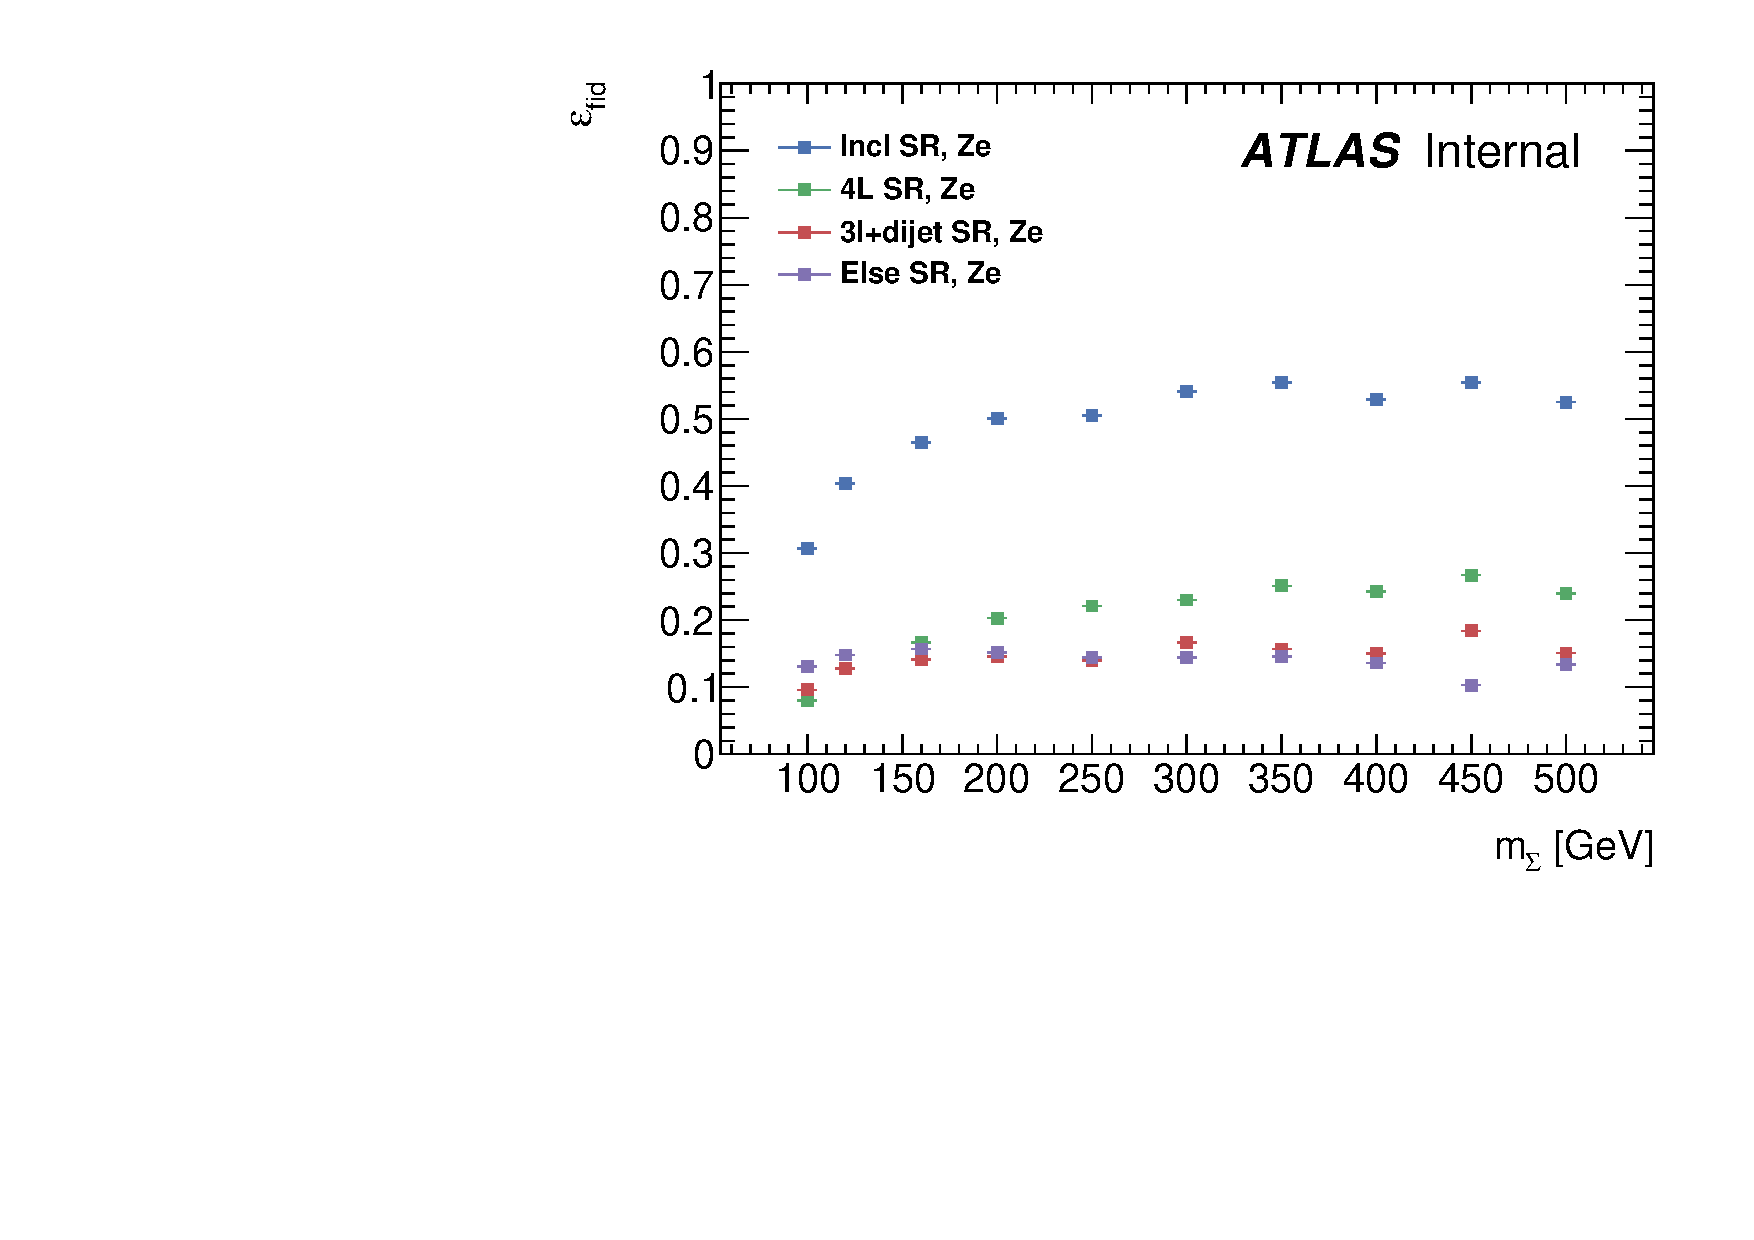
\includegraphics{figures/resonance/c_eff_fid_Ze_Seesaw}}
	}
	\subfloat[ $Z+e$, vector-like leptons] {
		\resizebox{0.4\textwidth}{!}{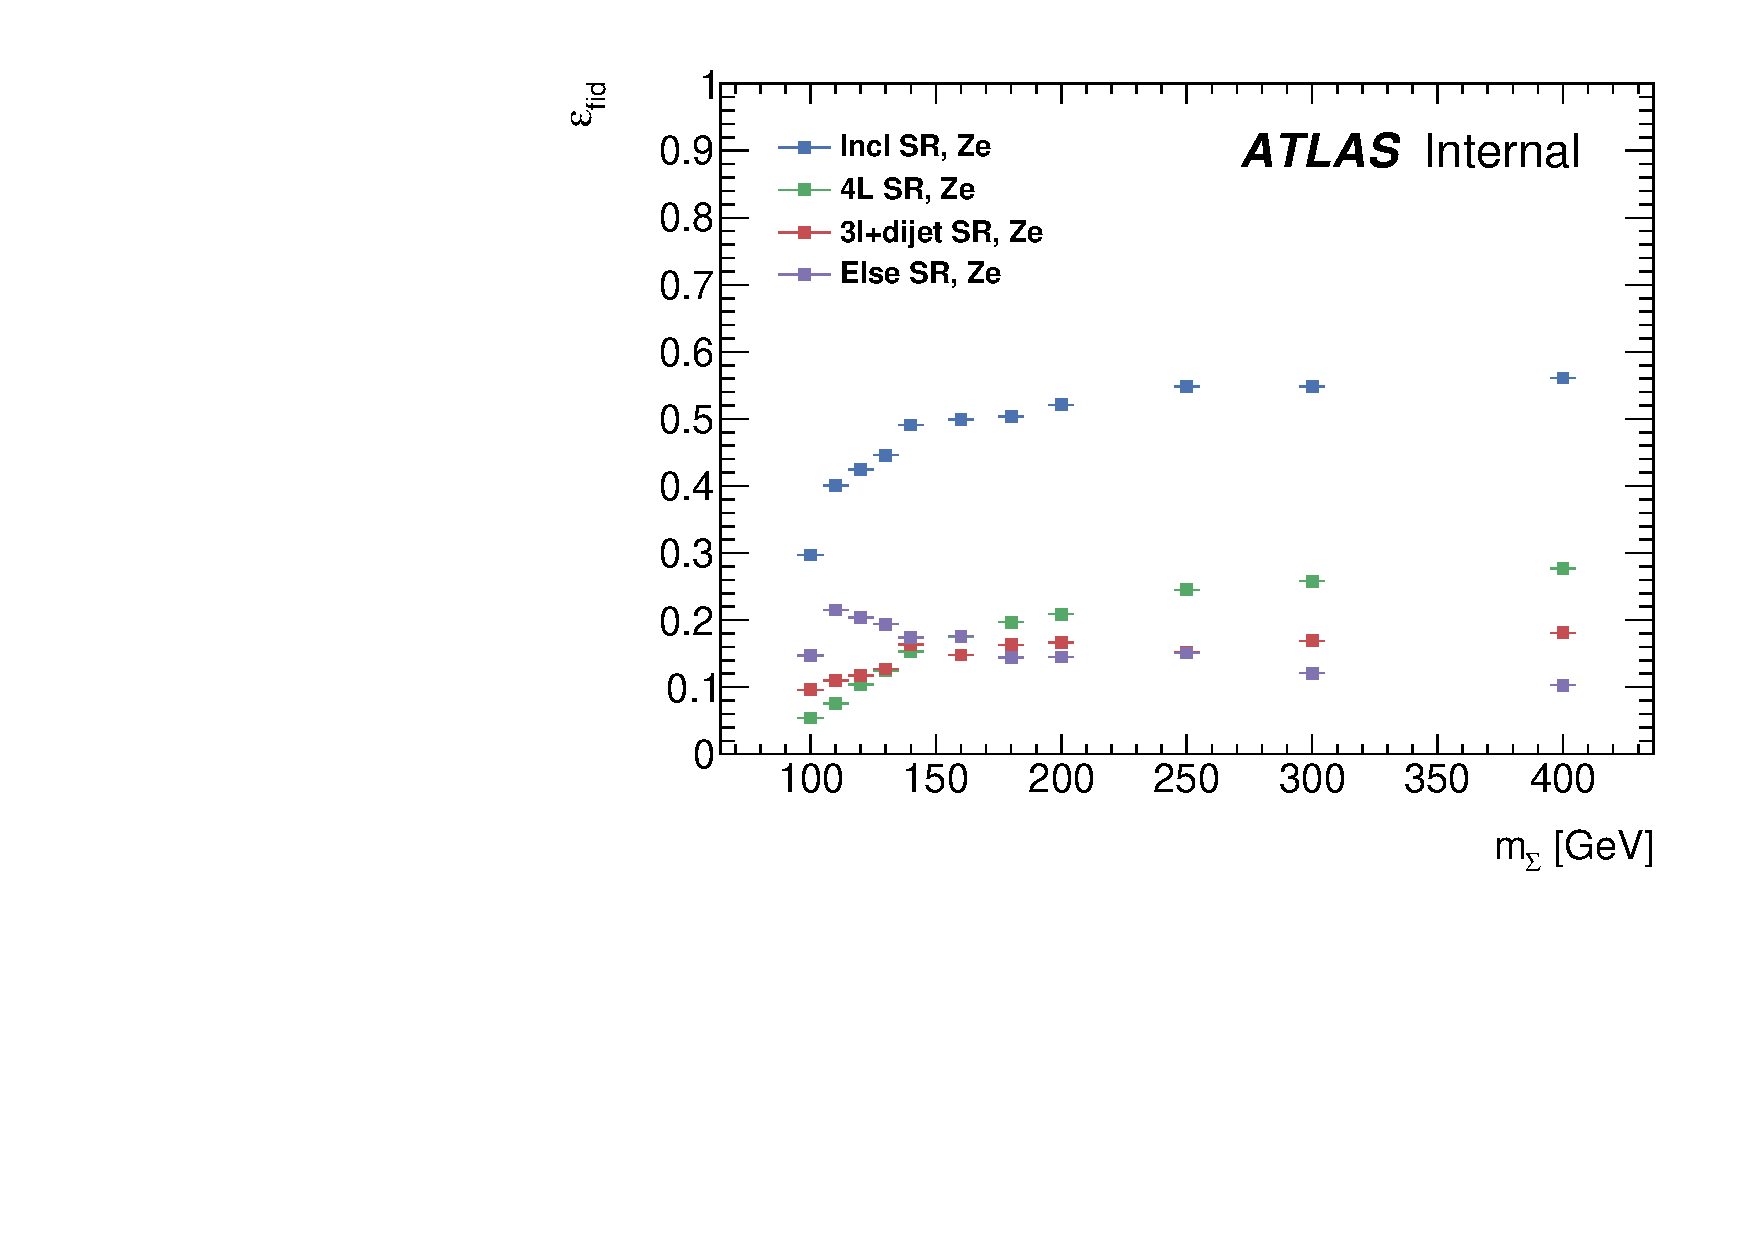
\includegraphics{figures/resonance/c_eff_fid_Ze_VLL}}
	} \\
	\subfloat[ $Z+\mu$, seesaw] {
		\resizebox{0.4\textwidth}{!}{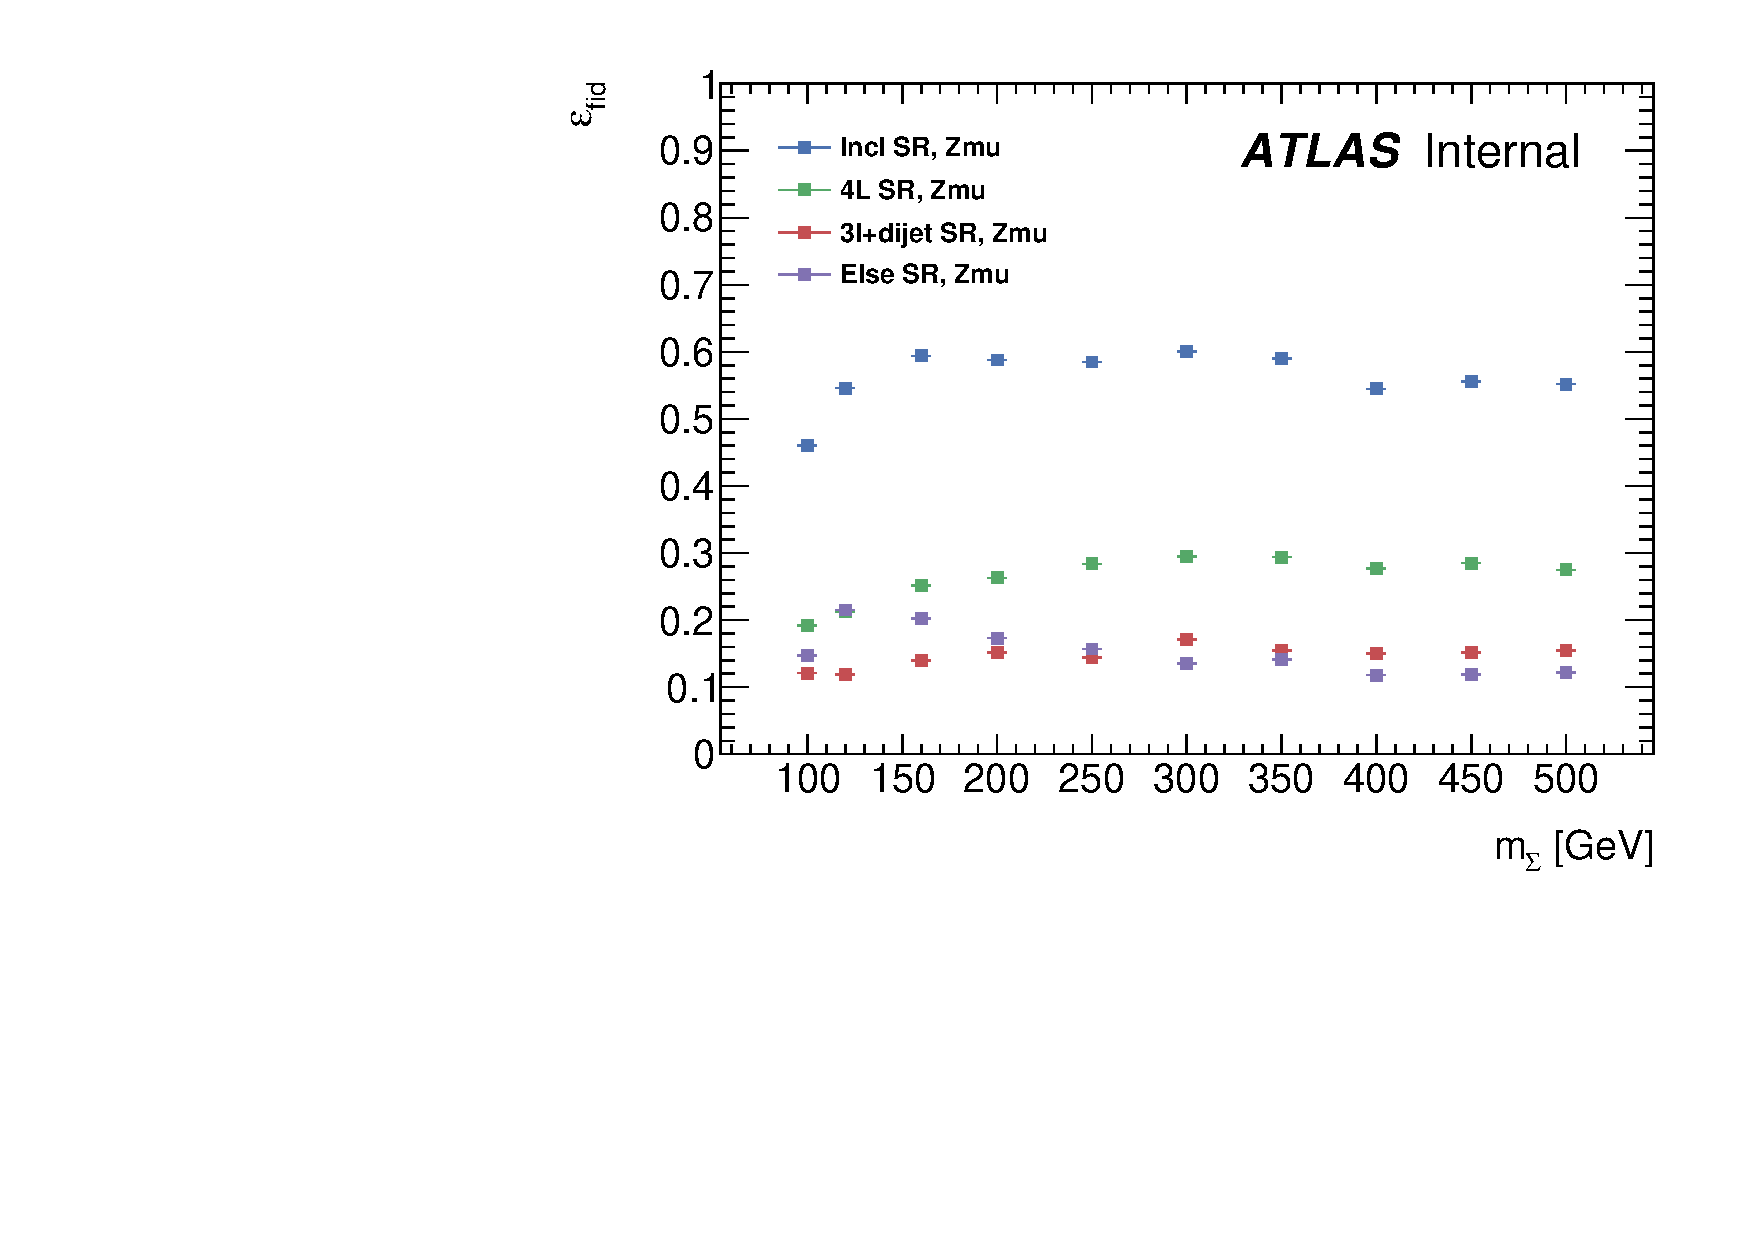
\includegraphics{figures/resonance/c_eff_fid_Zmu_Seesaw}}
	}
	\subfloat[ $Z+\mu$, vector-like leptons] {
		\resizebox{0.4\textwidth}{!}{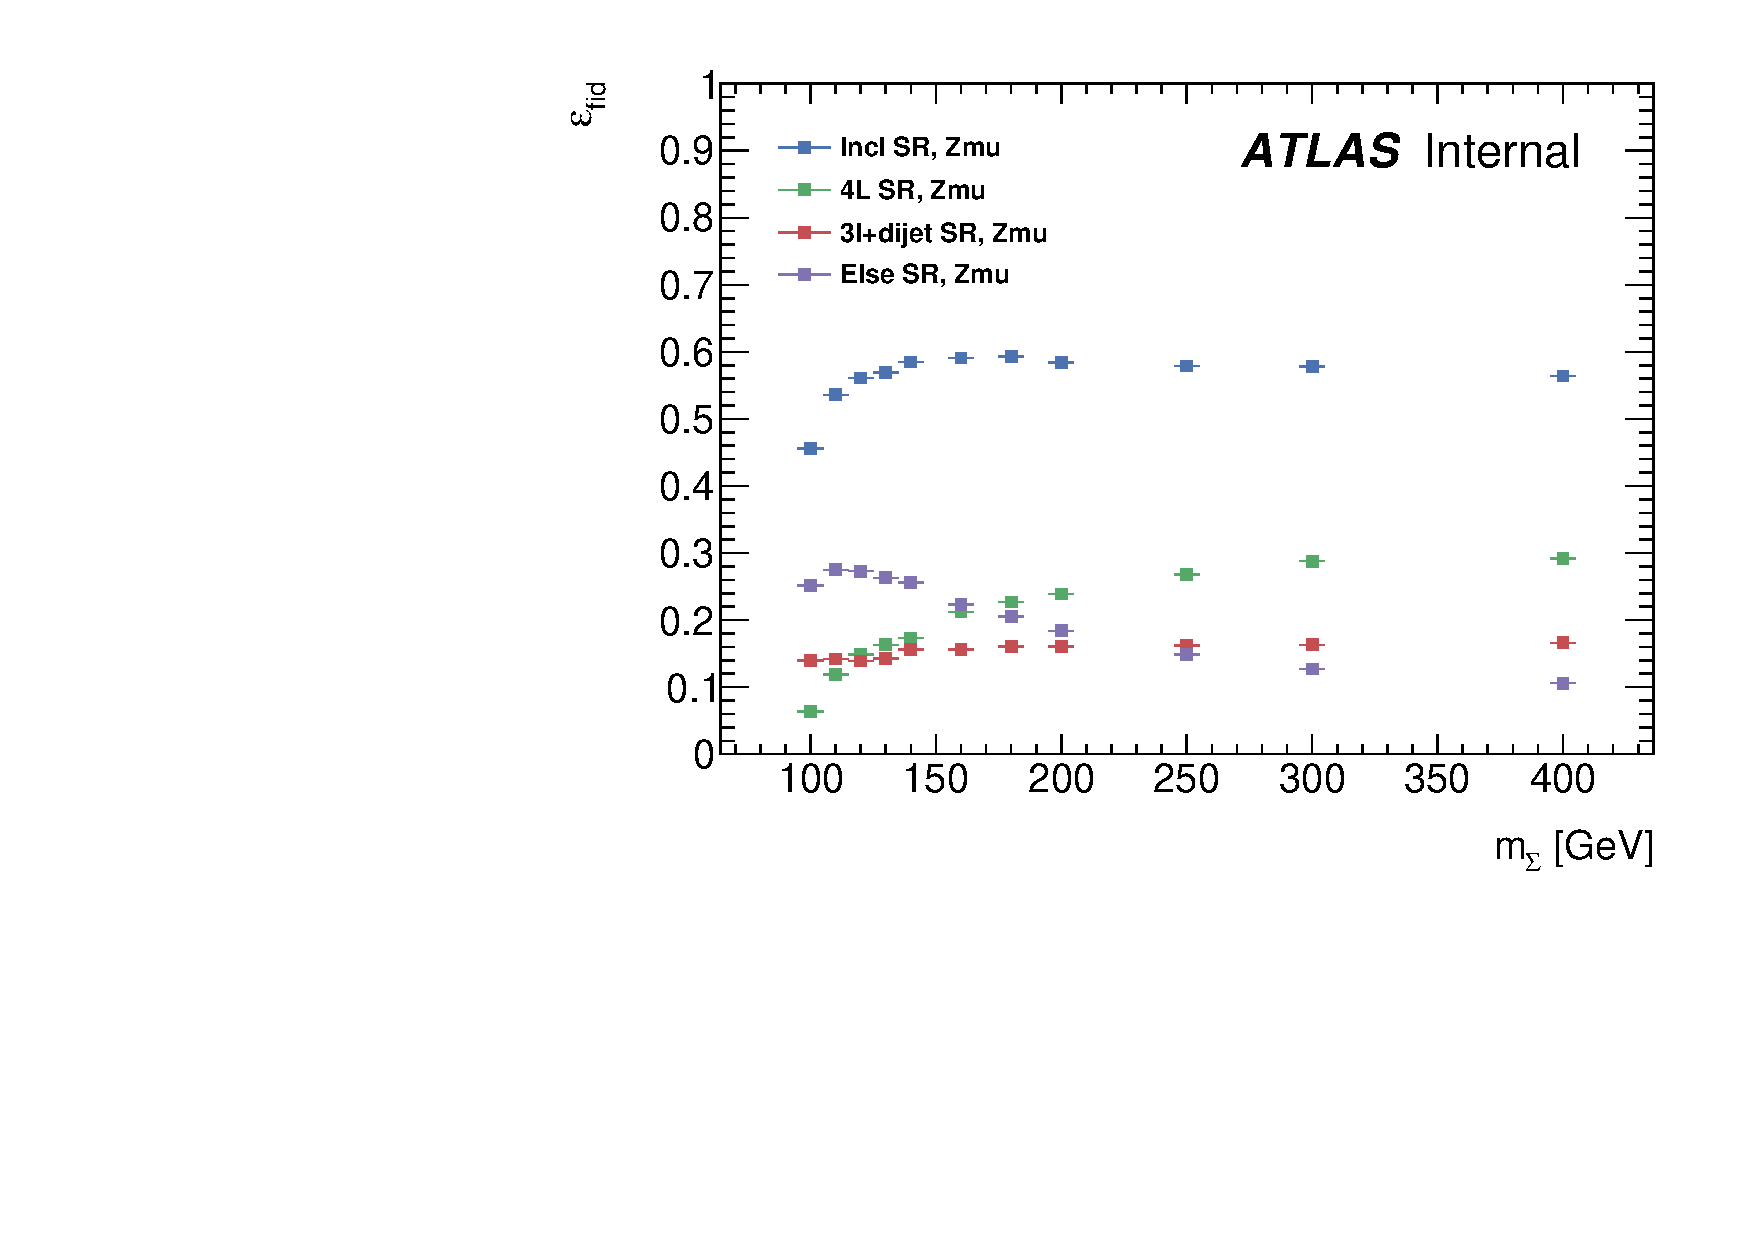
\includegraphics{figures/resonance/c_eff_fid_Zmu_VLL}}
	}
	\caption{Efficiencies of cuts defining each signal region on fiducial $Z(ll)l$ events at each simulated mass point. For the $Z+e$ signal regions, the branching fraction is set to be $BR(\lpm\rightarrow X+e/\nu_{e})=100\%$; similarly, for the $Z+\mu$ signal regions, the branching fraction is set to be $BR(\lpm\rightarrow X+\mu/\nu_{\mu})=100\%$.}
	\label{fig:fiducial-efficiencies-vs-mass}
\end{figure}


\clearpage

\section{Systematic Uncertainties}\label{sec:resonance-systematic-uncertainties}
The signal predictions and background estimates are assigned systematic uncertainties from several sources. In approximate order of significance, these are:

\begin{itemize}
	\item \textbf{Diboson shape uncertainty}: A systematic uncertainty is assigned to the modeling of $\deltam$ spectra of the diboson backgrounds by comparing \sherpa\ to \powheg. \sherpa\ is used as a central value, with uncertainty given by the symmetric difference between \sherpa\ and \powheg. As described below in section~\ref{sec:resonance-background-model}, the shapes for the $\fourl$ and $\threelo$ signal regions are taken from the inclusive signal region, so the corresponding uncertainties are derived only from the inclusive and $\threeljj$ signal regions. The comparison for the $WZ$ background is shown in figure~\ref{fig:systematic-WZ-shape}. The implementation of this uncertainty in the fit-based limit section is discussed in more detail in section~\ref{sec:fit-limits-systematic-uncertainties}; briefly, the uncertainty is included as a gaussian-distributed nuisance parameter interpolating between the two fits estimated from the two generators.

	In the case of the $ZZ$ background, this procedure is complicated by the fact that the \powheg\ sample is filtered to remove events with same-flavor, opposite-sign lepton pairs with $m_{l^+l^-}<4~\mbox{GeV}$ (\texttt{mll4}). In order to compare the samples in a common phase space, the \texttt{mll4} filter is emulated on the \sherpa\ sample by rejecting events that contain a same-flavor, opposite-sign pair of truth leptons with $m_{l^+l^-}<4~\mbox{GeV}$. \sherpa, \sherpa\ with \texttt{mll4} filter, and \powheg\ are compared in figure~\ref{fig:ZZ-mll4}. The events from the \powheg\ sample are weighted using the ratio of \sherpa\ to \sherpa+\texttt{mll4}. The final comparison of background shapes is shown in figure~\ref{fig:systematic-ZZ-shape}.

	\begin{figure}[h]
		\centering
		\subfloat[ Inclusive SR, $Z+e$] {
			\resizebox{2.5in}{!}{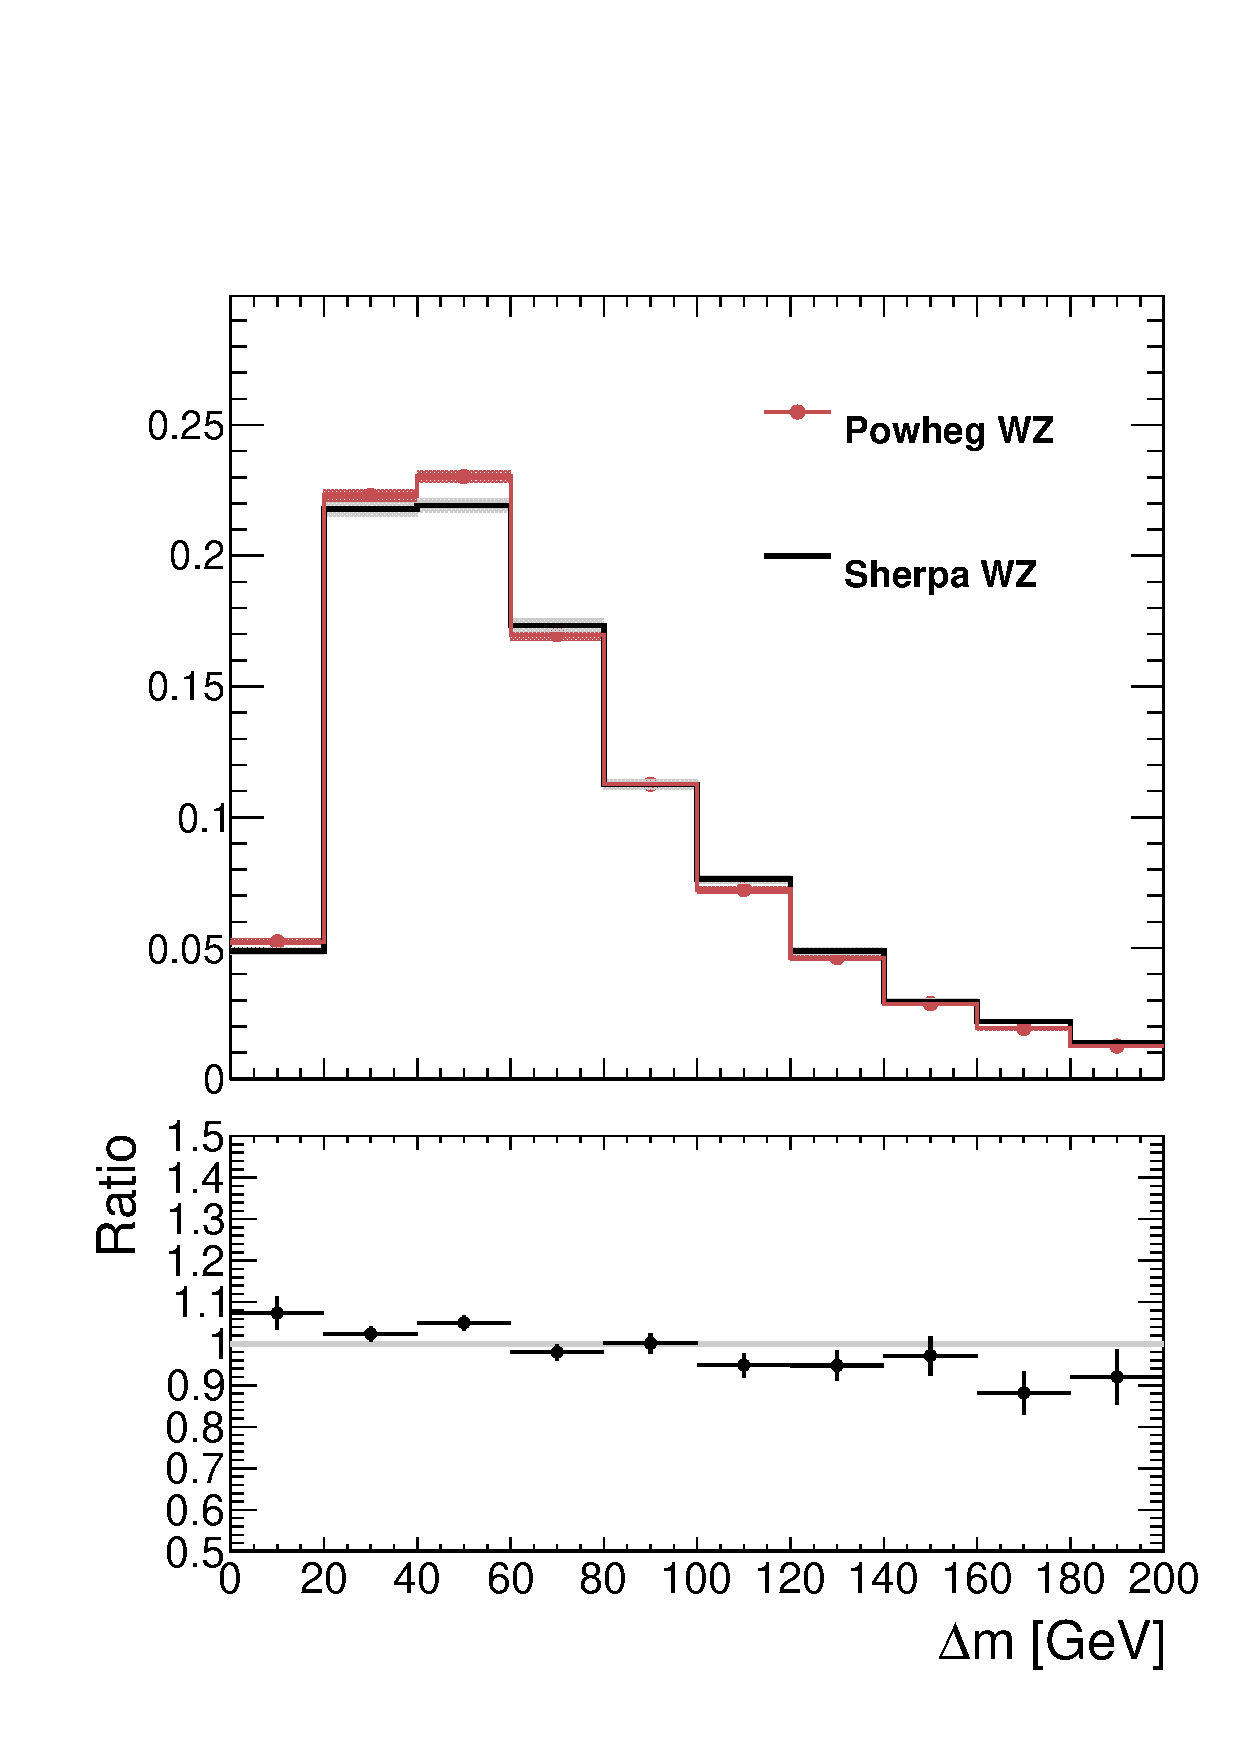
\includegraphics{figures/resonance/c_systematics_WZShape_Ze_InclusiveNoM3L_WZ.pdf}}
		}
		\subfloat[ $\threeljj$ SR, $Z+e$] {
			\resizebox{2.5in}{!}{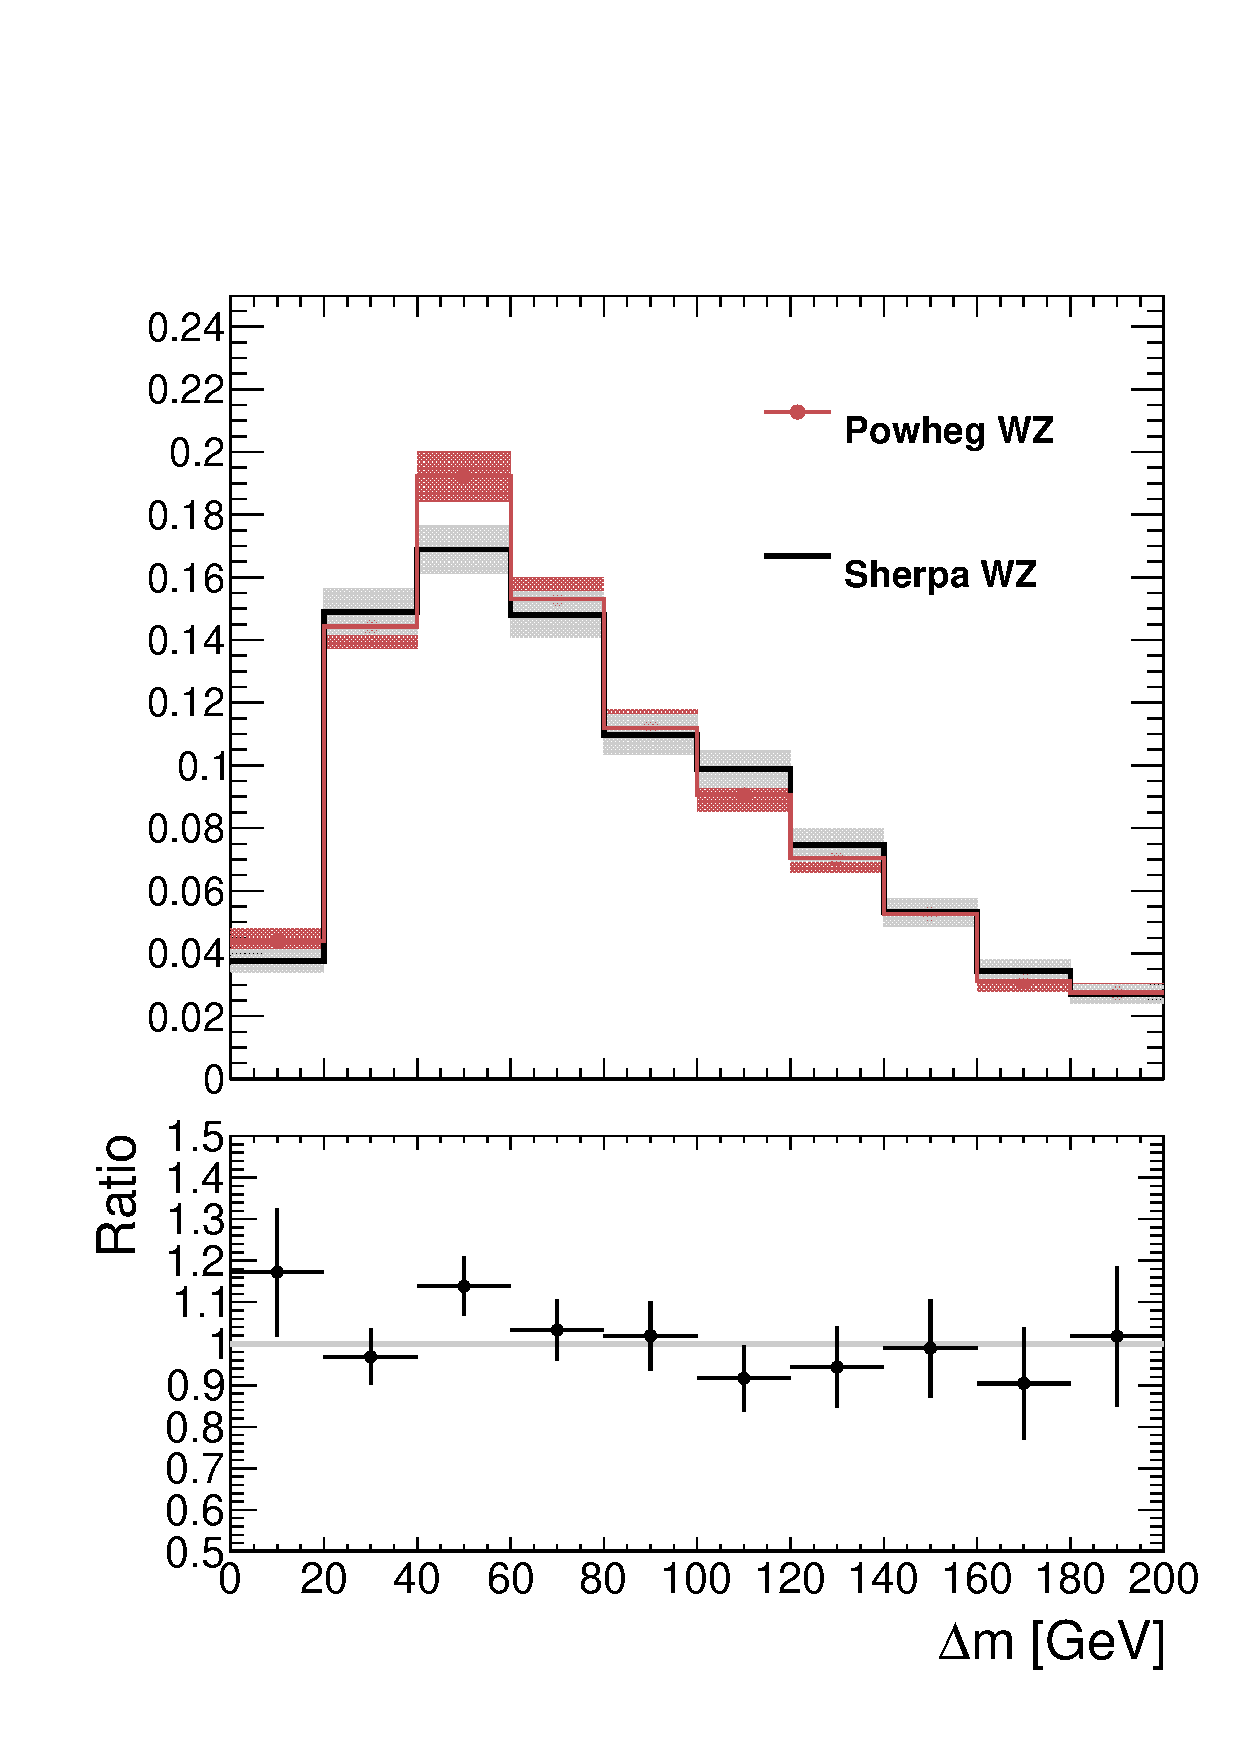
\includegraphics{figures/resonance/c_systematics_WZShape_Ze_ThreeLDijetNoM3L_WZ.pdf}}
		} \\
		\subfloat[ Inclusive SR, $Z+\mu$] {
			\resizebox{2.5in}{!}{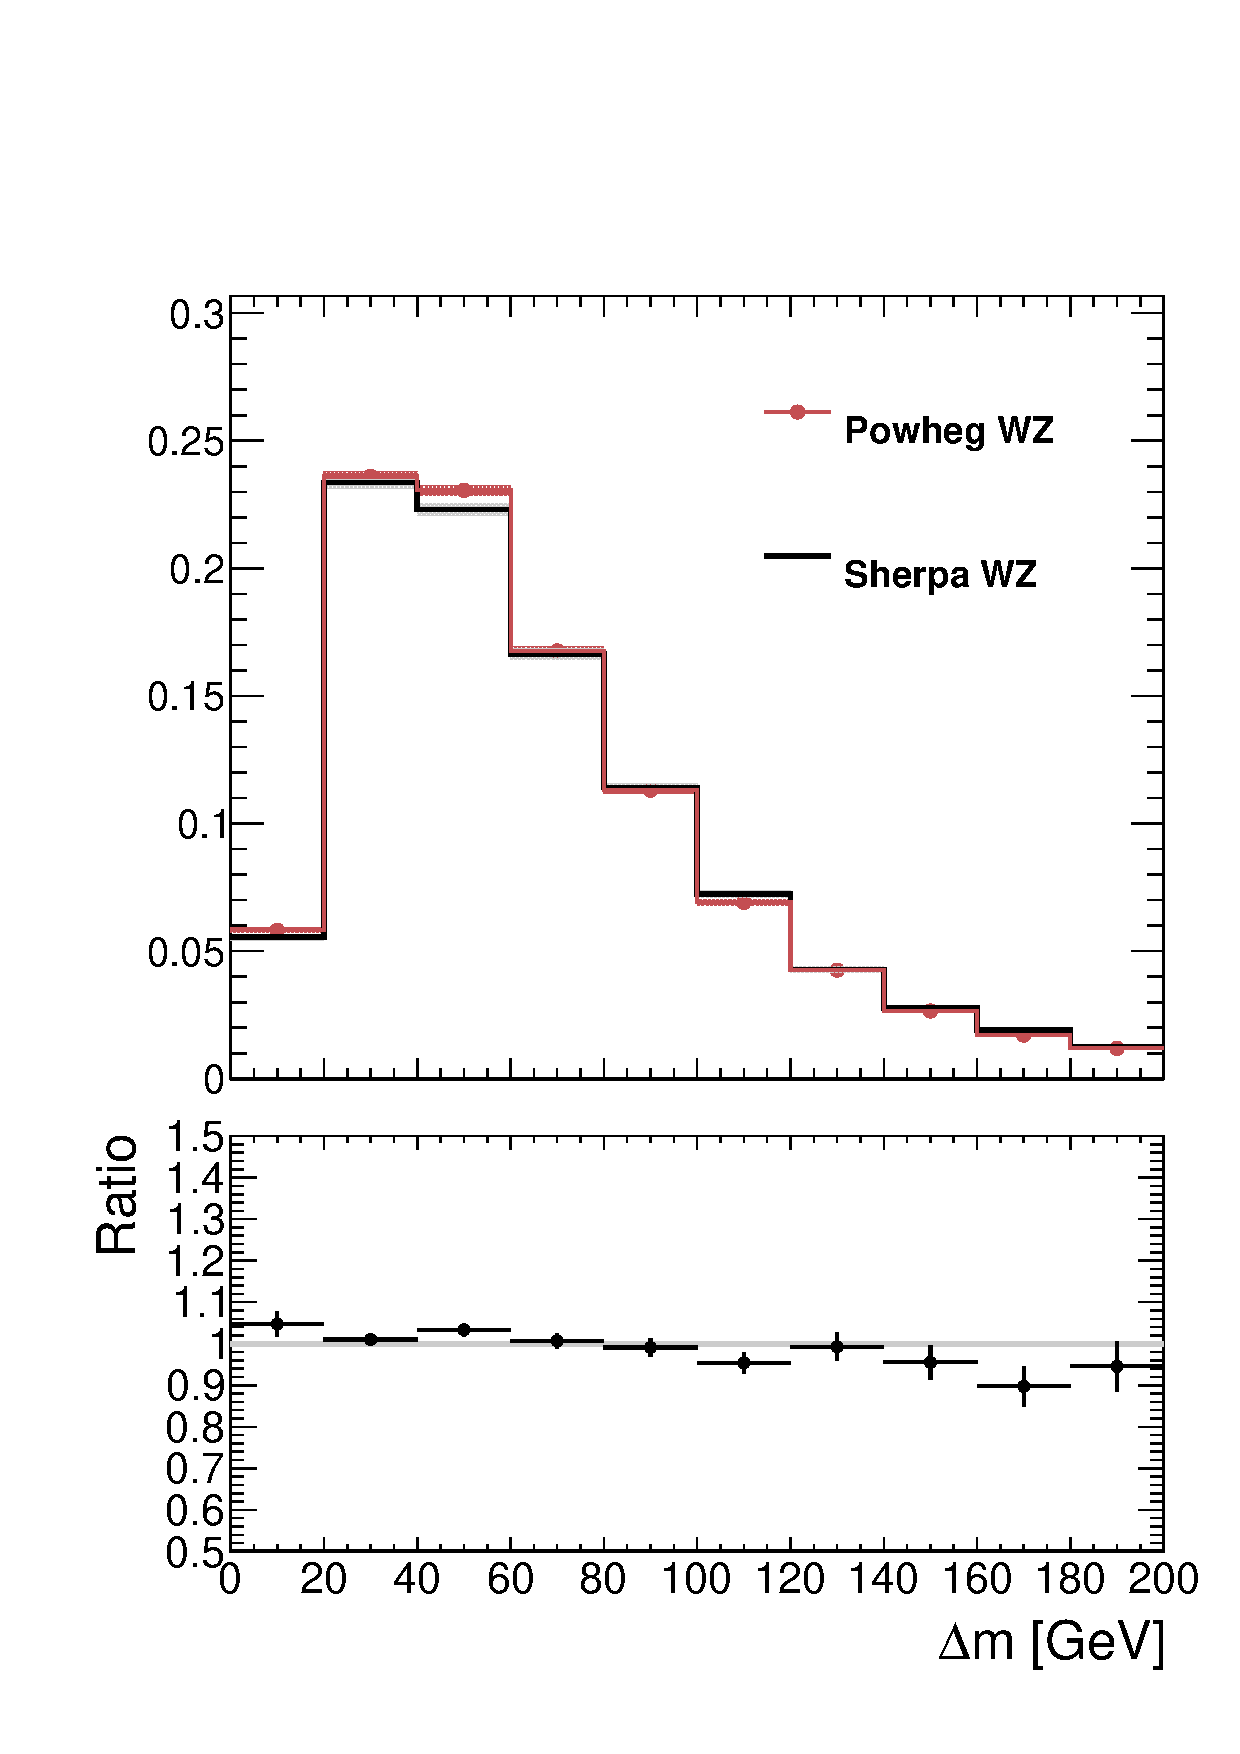
\includegraphics{figures/resonance/c_systematics_WZShape_Zmu_InclusiveNoM3L_WZ.pdf}}
		}
		\subfloat[ $\threeljj$ SR, $Z+\mu$] {
			\resizebox{2.5in}{!}{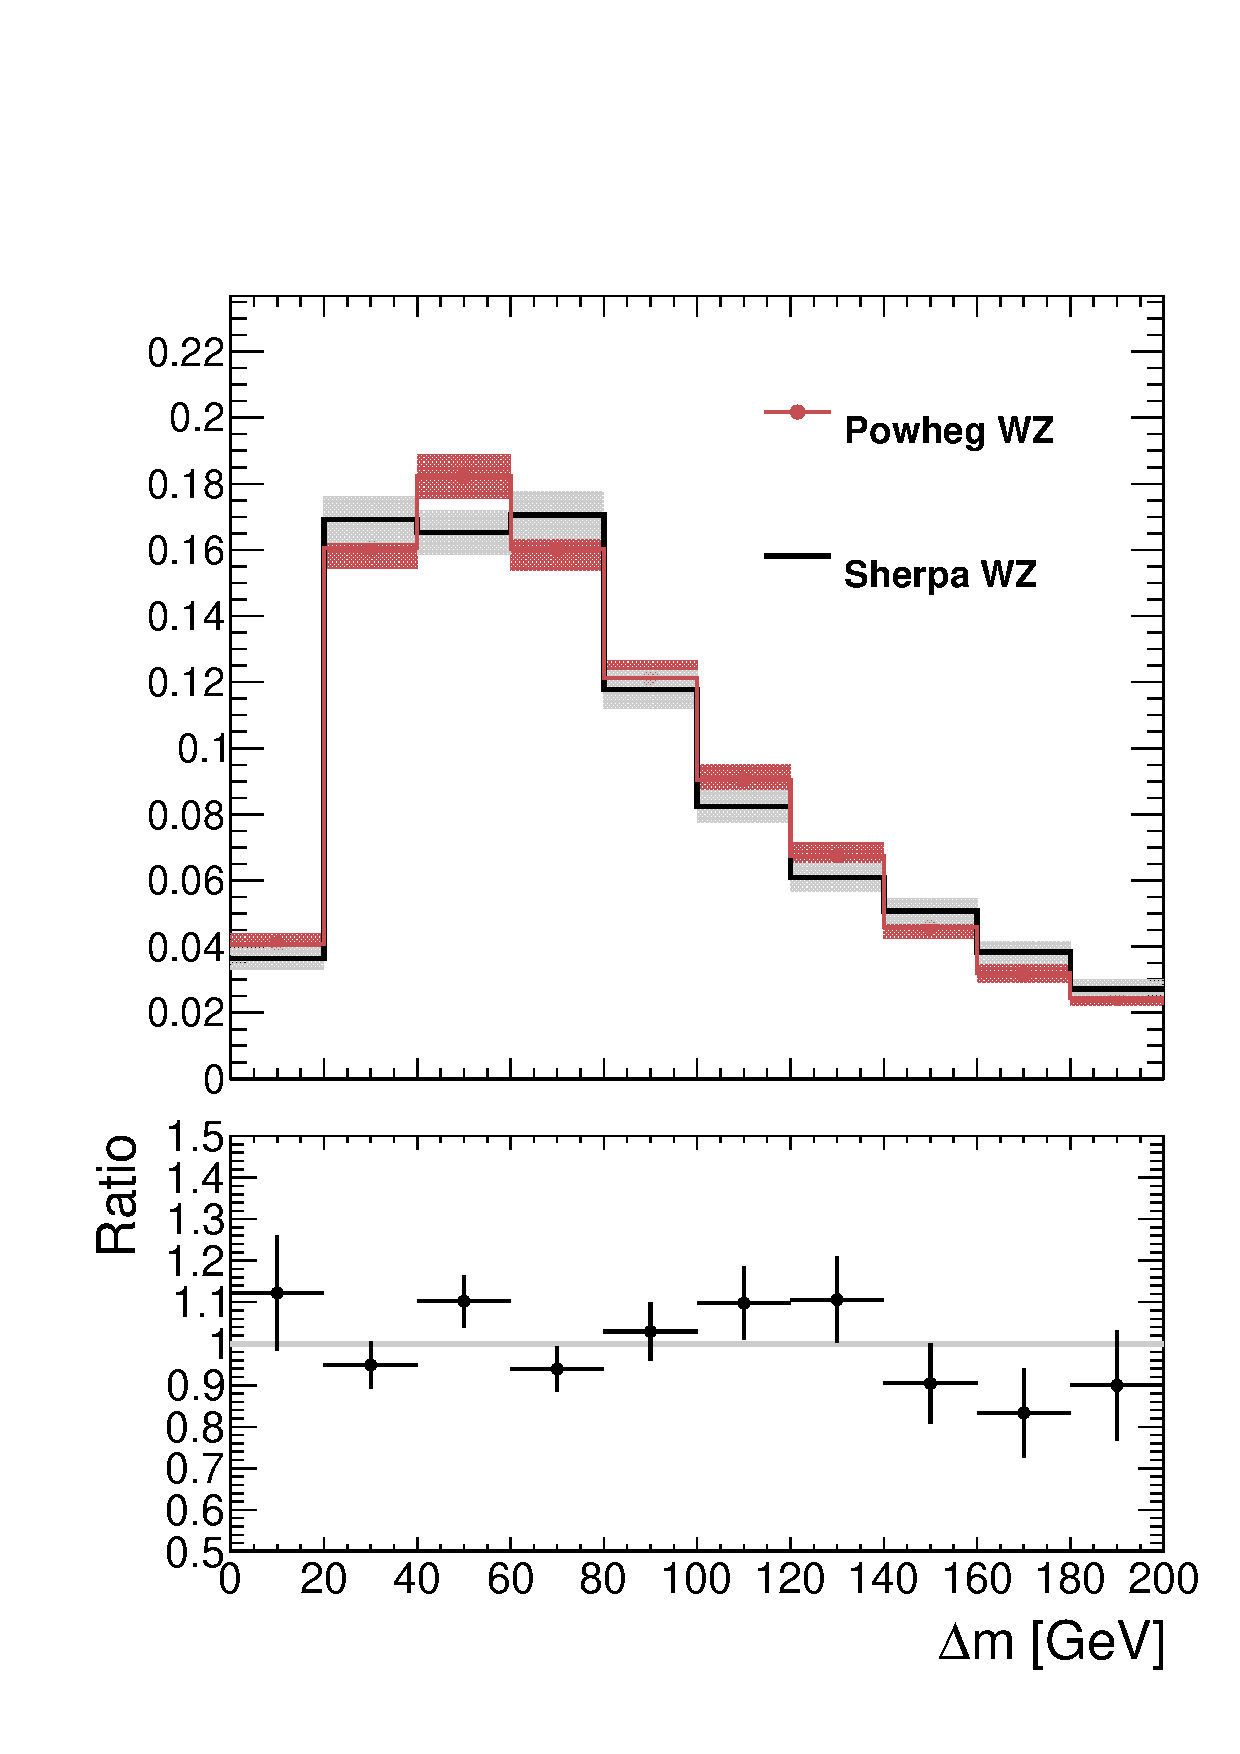
\includegraphics{figures/resonance/c_systematics_WZShape_Zmu_ThreeLDijetNoM3L_WZ.pdf}}
		}
		\caption{Comparison of the $\deltam$ distributions between \powheg\ and \sherpa\ for the $WZ$ backgrounds. The 4L signal region is omitted due to the negligible number of $WZ$ events with four leptons.}
		\label{fig:systematic-WZ-shape}
	\end{figure}

	\begin{figure}[h]
		\centering
		\subfloat[ Inclusive SR, $Z+e$] {
			\resizebox{2.5in}{!}{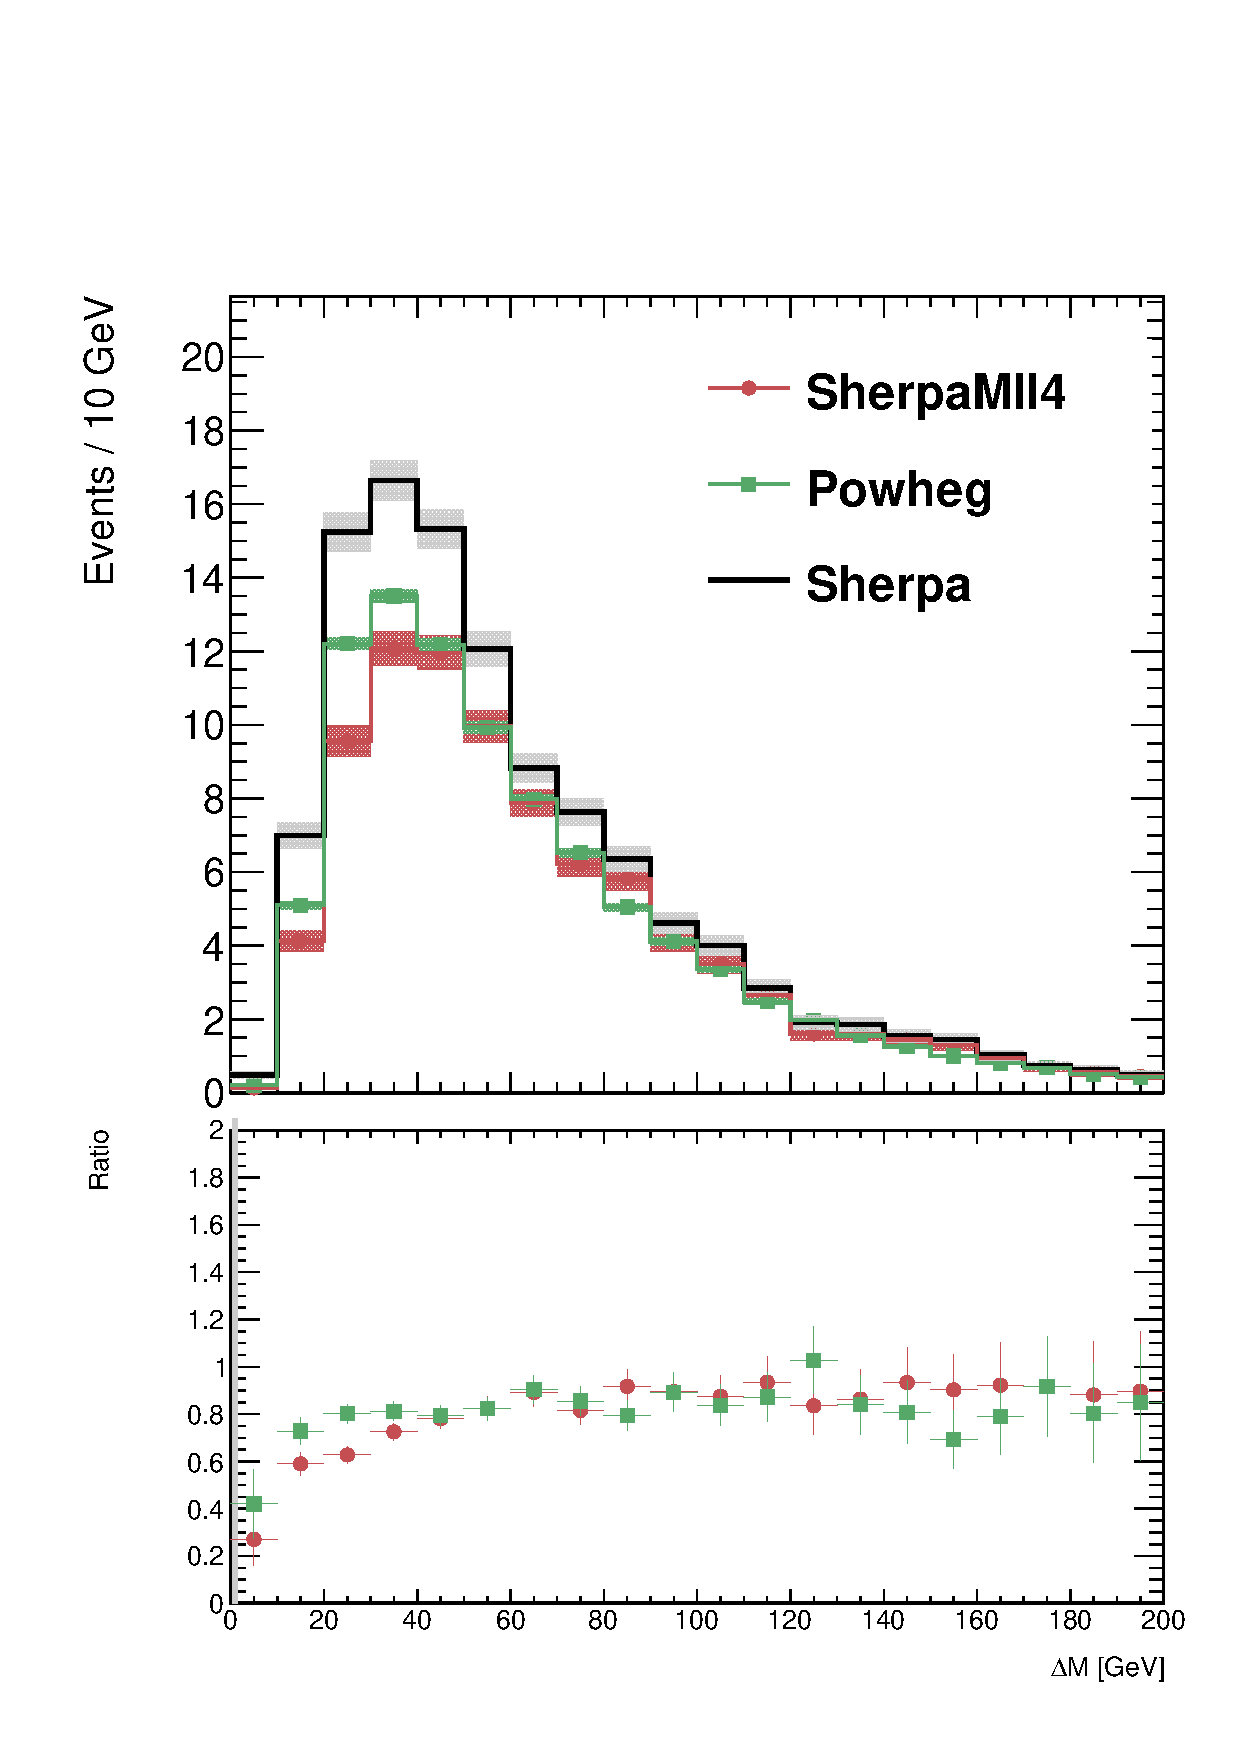
\includegraphics{figures/resonance/c_systematics_ZZShape_DeltaM_Ze_InclusiveNoM3L}}
		}
		\subfloat[ $\threeljj$ SR, $Z+e$] {
			\resizebox{2.5in}{!}{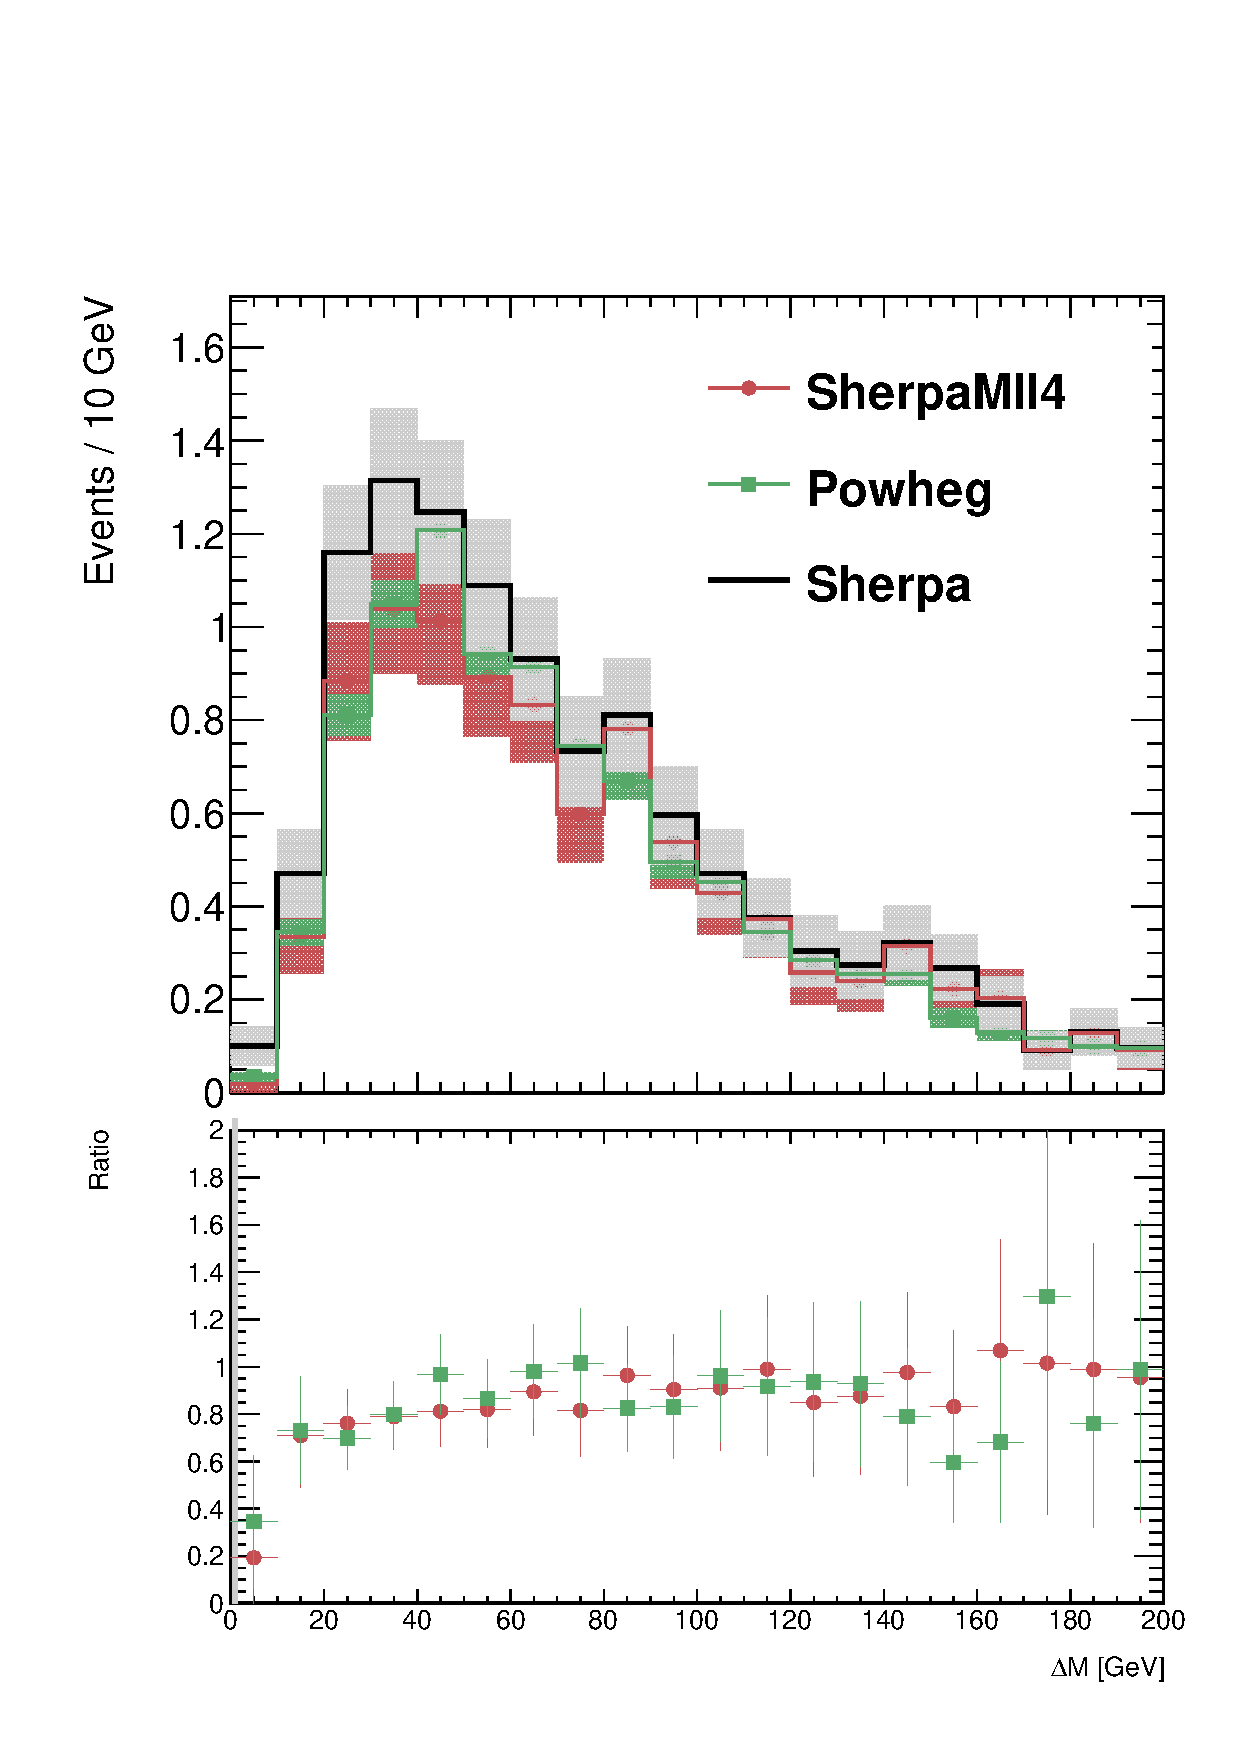
\includegraphics{figures/resonance/c_systematics_ZZShape_DeltaM_Ze_ThreeLDijetNoM3L}}
		} \\
		\subfloat[ Inclusive SR, $Z+\mu$] {
			\resizebox{2.5in}{!}{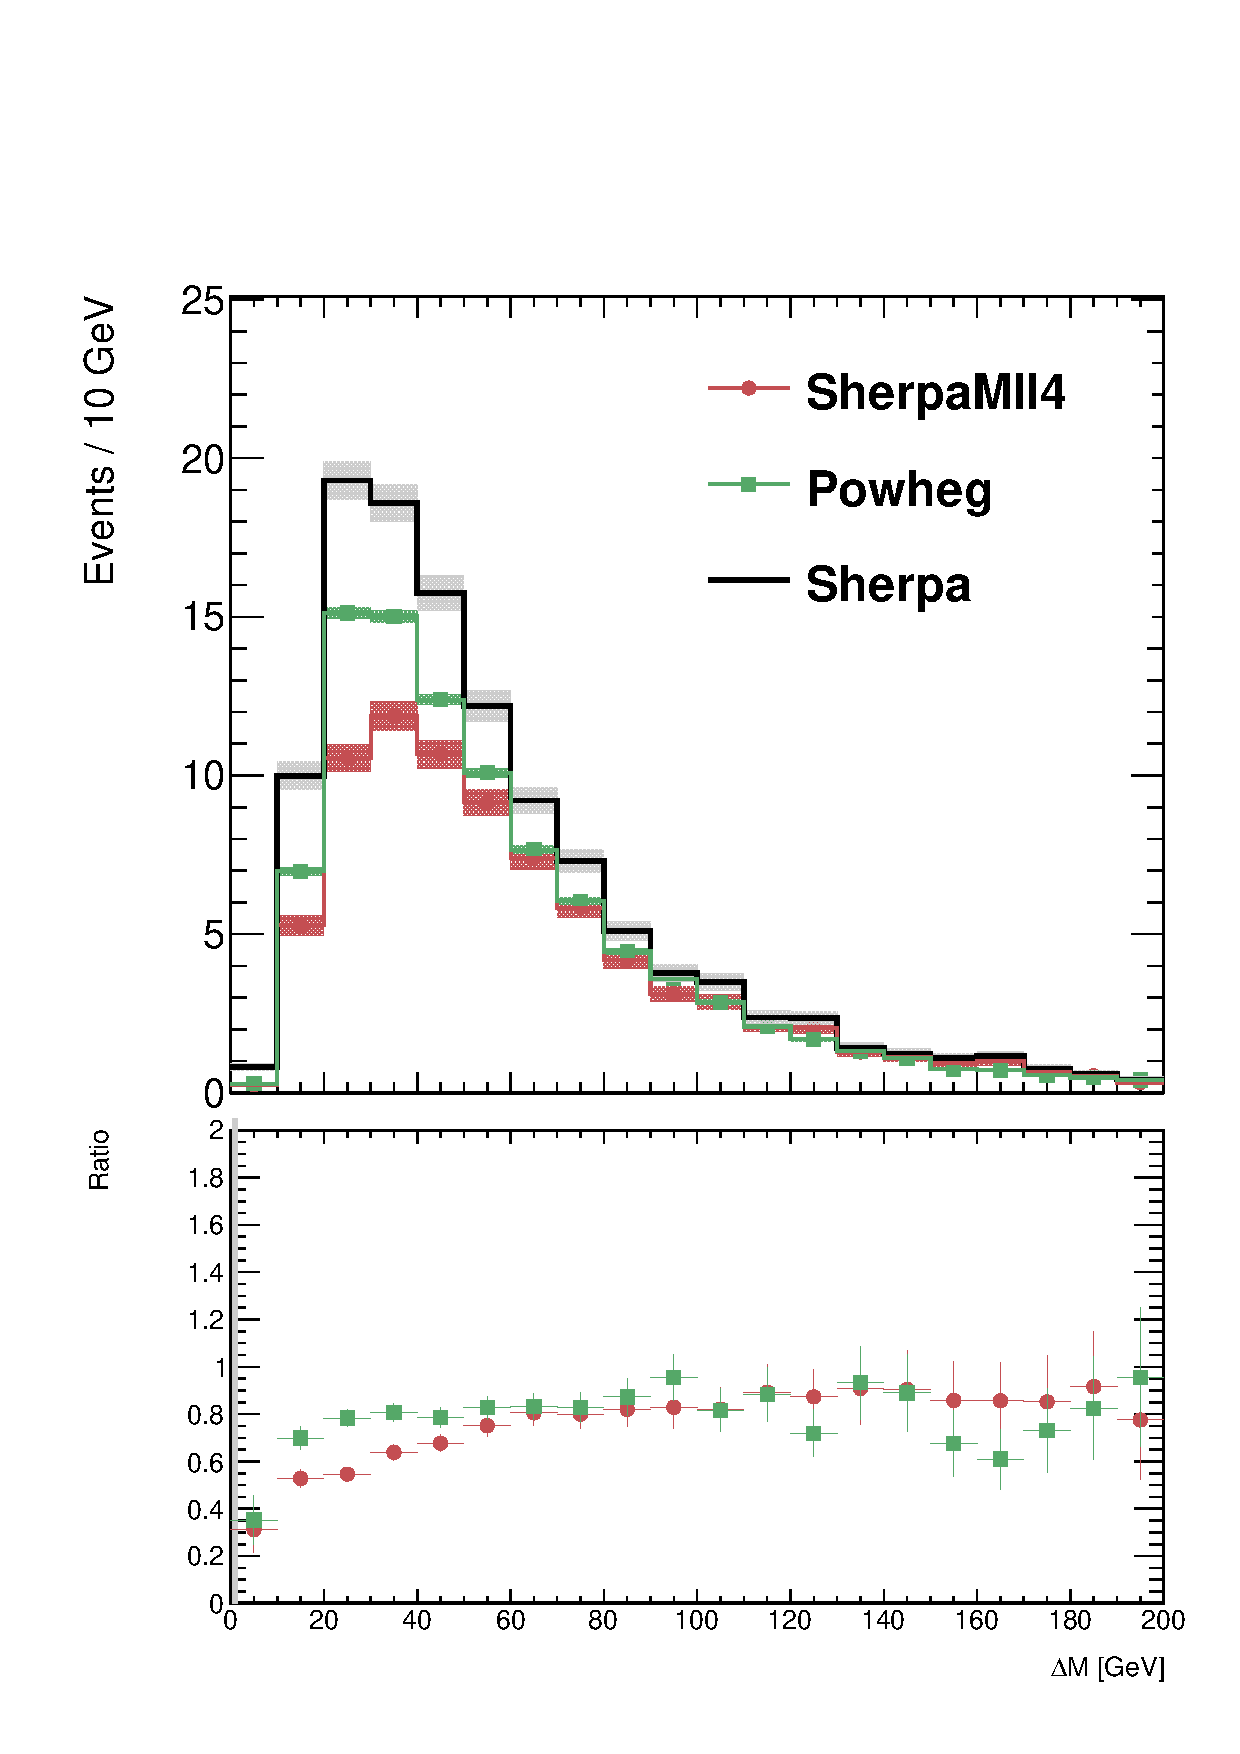
\includegraphics{figures/resonance/c_systematics_ZZShape_DeltaM_Zmu_InclusiveNoM3L}}
		}
		\subfloat[ $\threeljj$ SR, $Z+\mu$] {
			\resizebox{2.5in}{!}{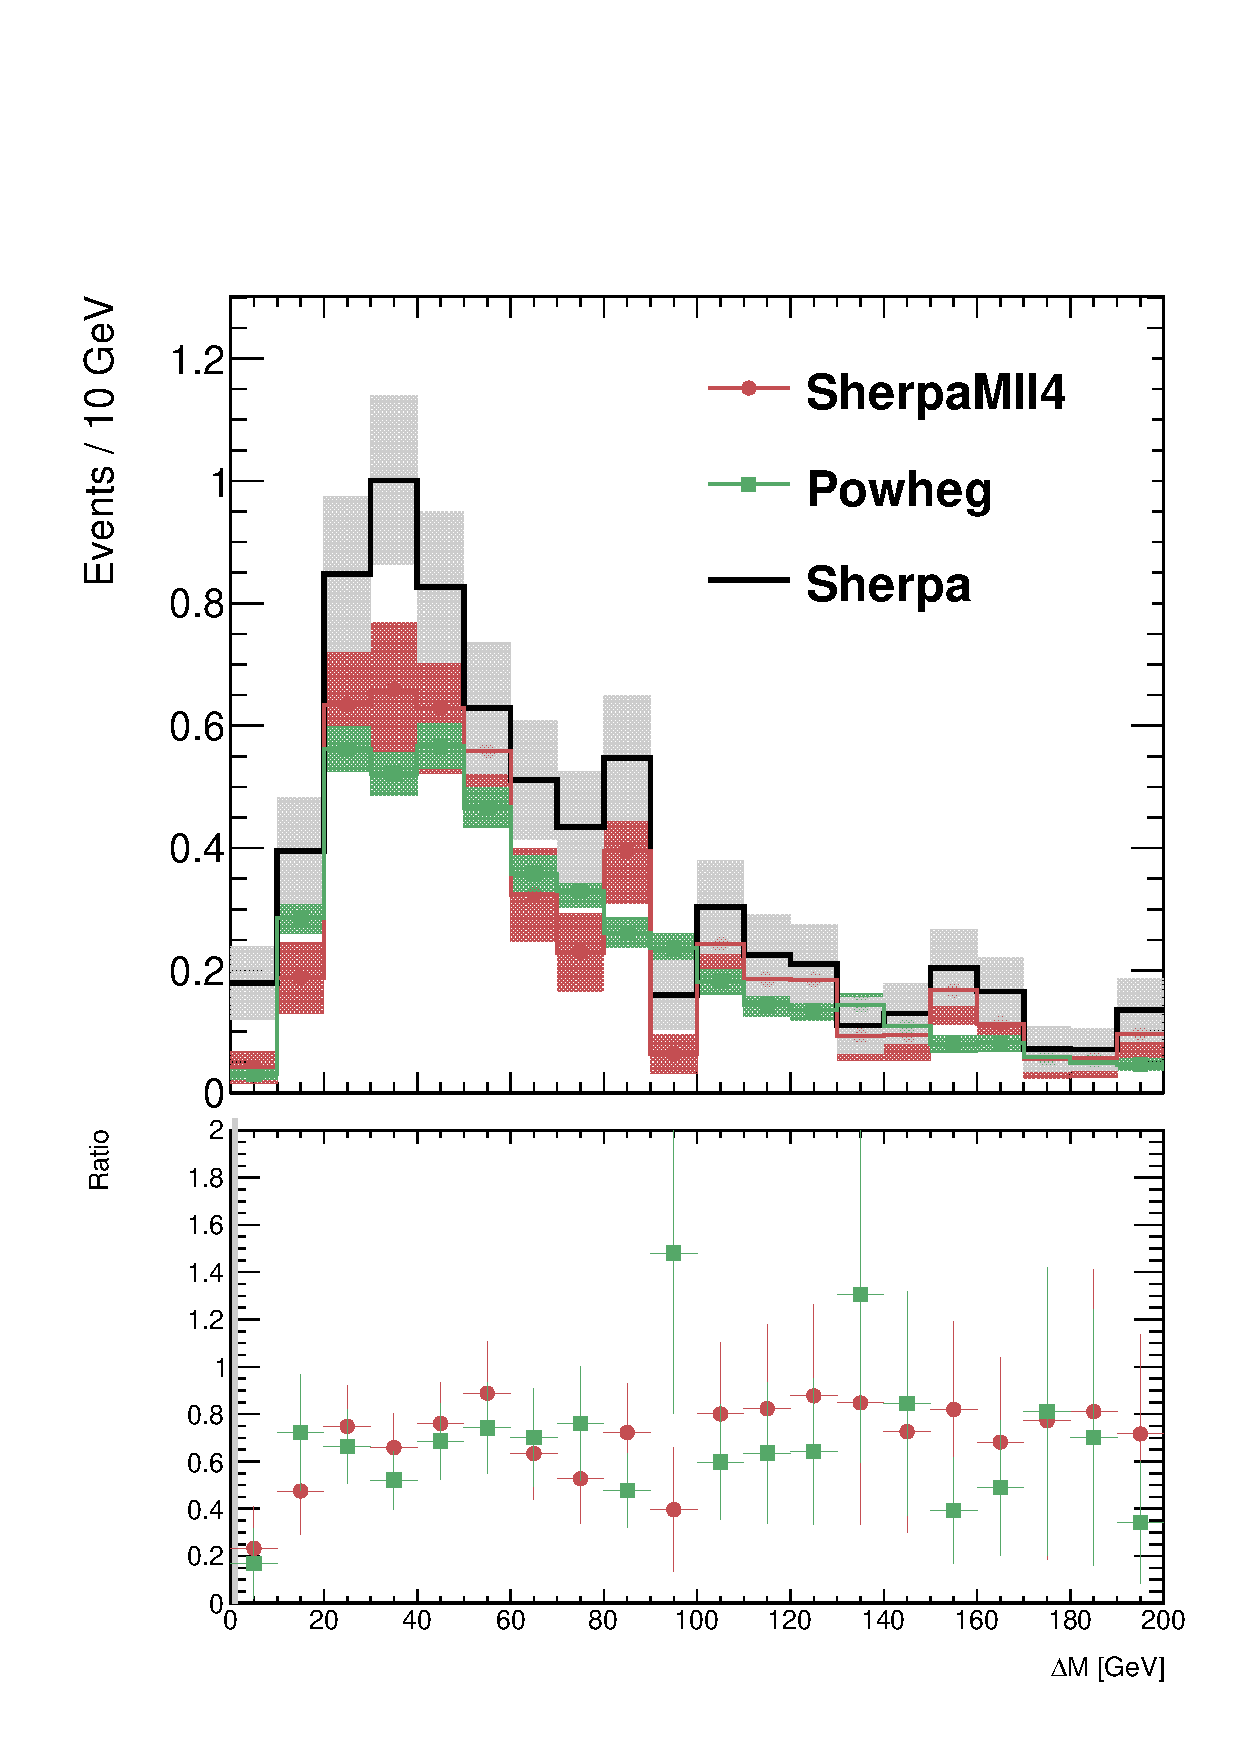
\includegraphics{figures/resonance/c_systematics_ZZShape_DeltaM_Zmu_ThreeLDijetNoM3L}}
		}
		\caption{Comparison of \sherpa, \sherpa\ with mll4 filter, and \powheg.}
		\label{fig:ZZ-mll4}
	\end{figure}
	

	\begin{figure}[h]
		\centering
		\subfloat[ Inclusive SR, $Z+e$] {
			\resizebox{2.5in}{!}{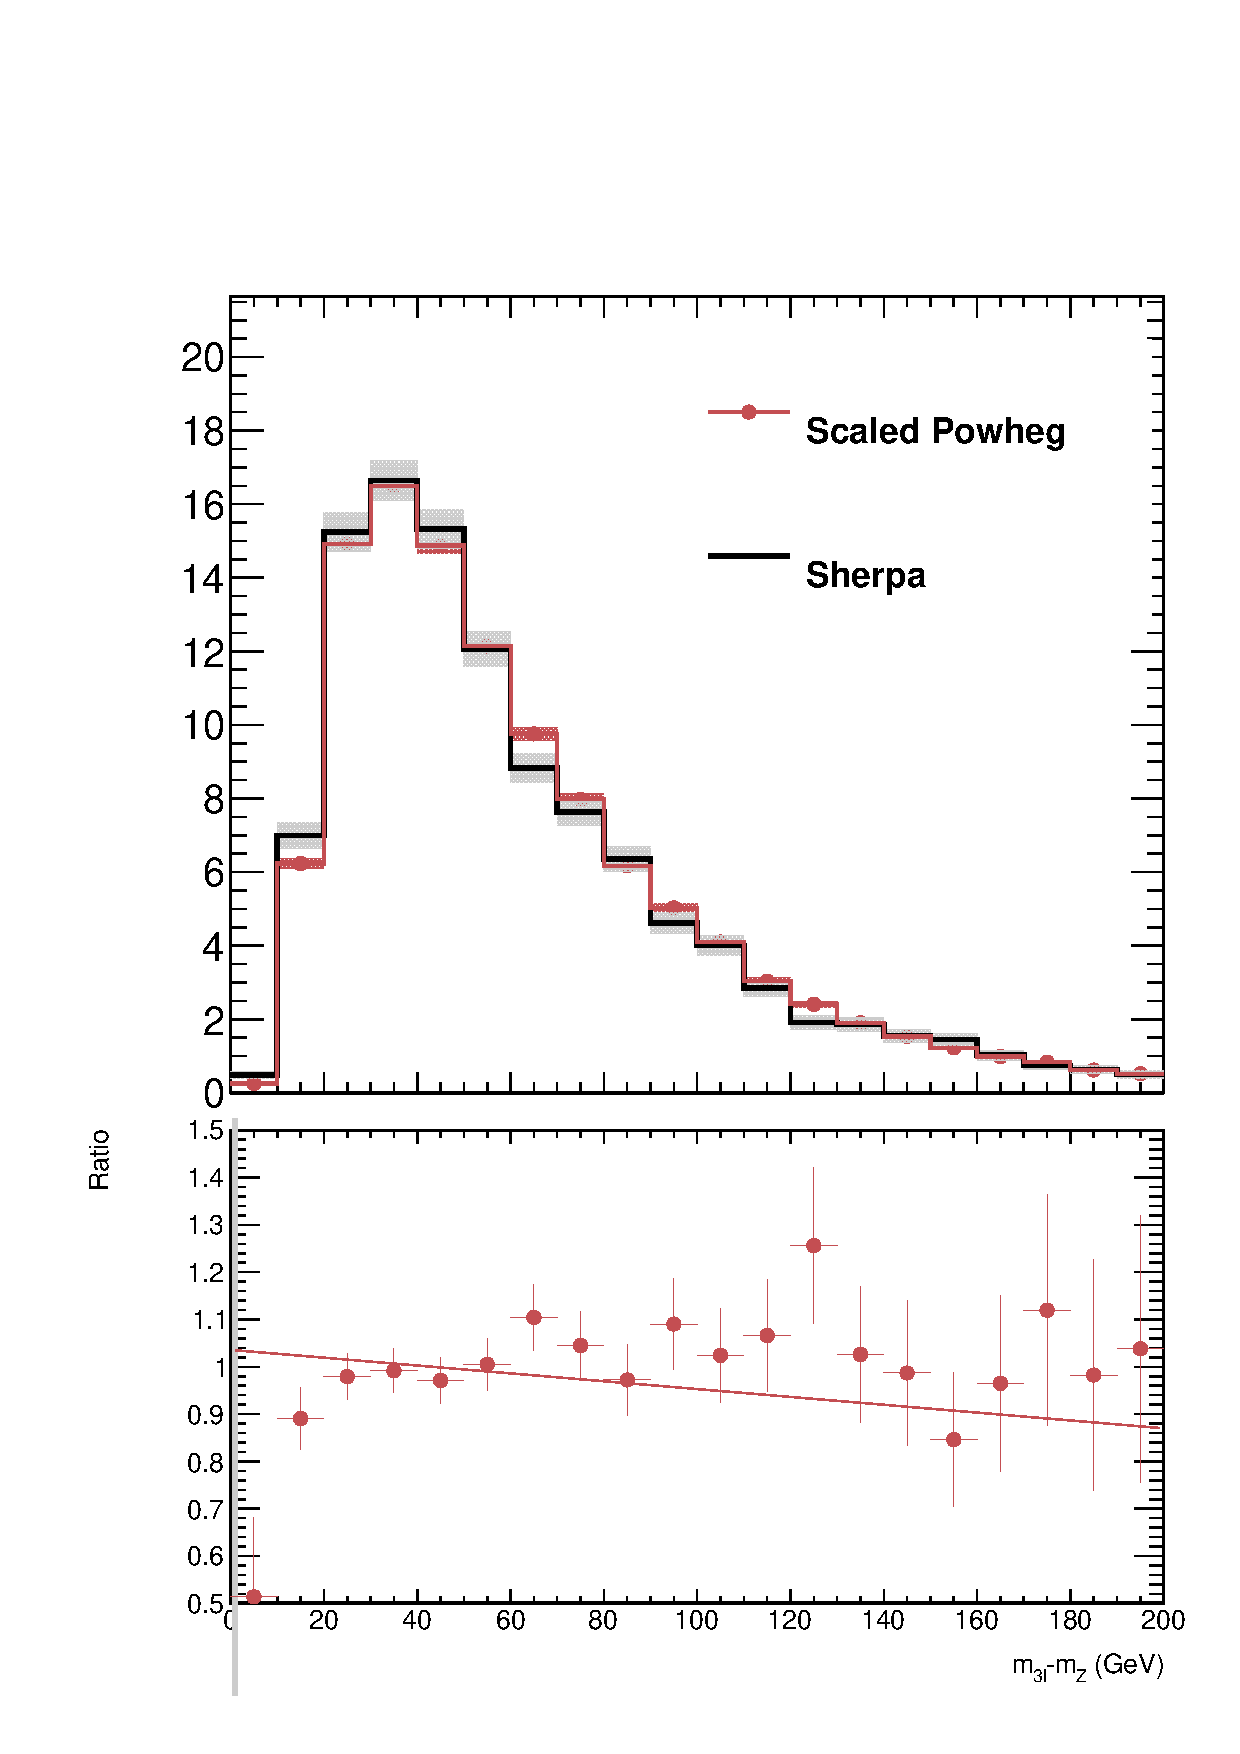
\includegraphics{figures/resonance/c_systematics_ZZShapeSyst_Ze_InclusiveNoM3L.pdf}}
		}
		\subfloat[ $\threeljj$ SR, $Z+e$] {
			\resizebox{2.5in}{!}{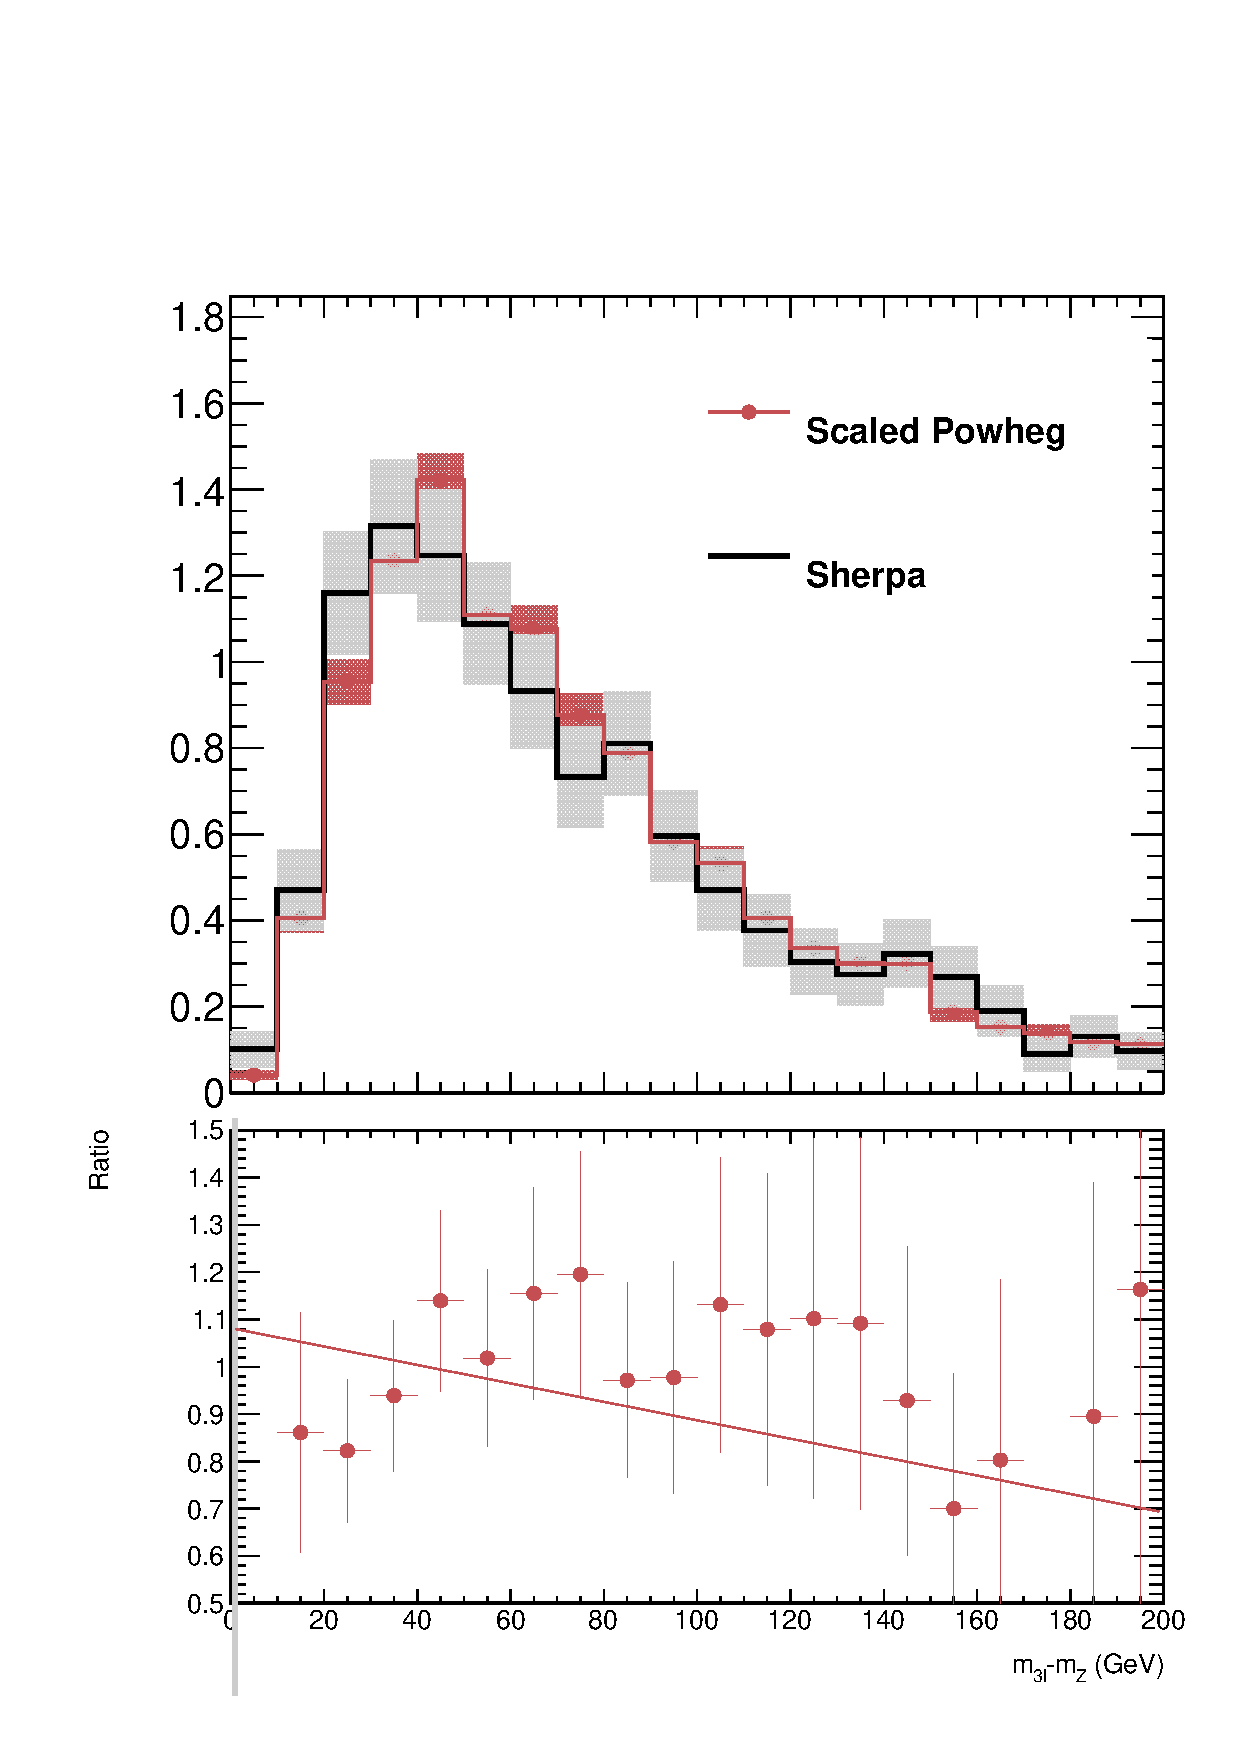
\includegraphics{figures/resonance/c_systematics_ZZShapeSyst_Ze_ThreeLDijetNoM3L.pdf}}
		} \\
		\subfloat[ Inclusive SR, $Z+\mu$] {
			\resizebox{2.5in}{!}{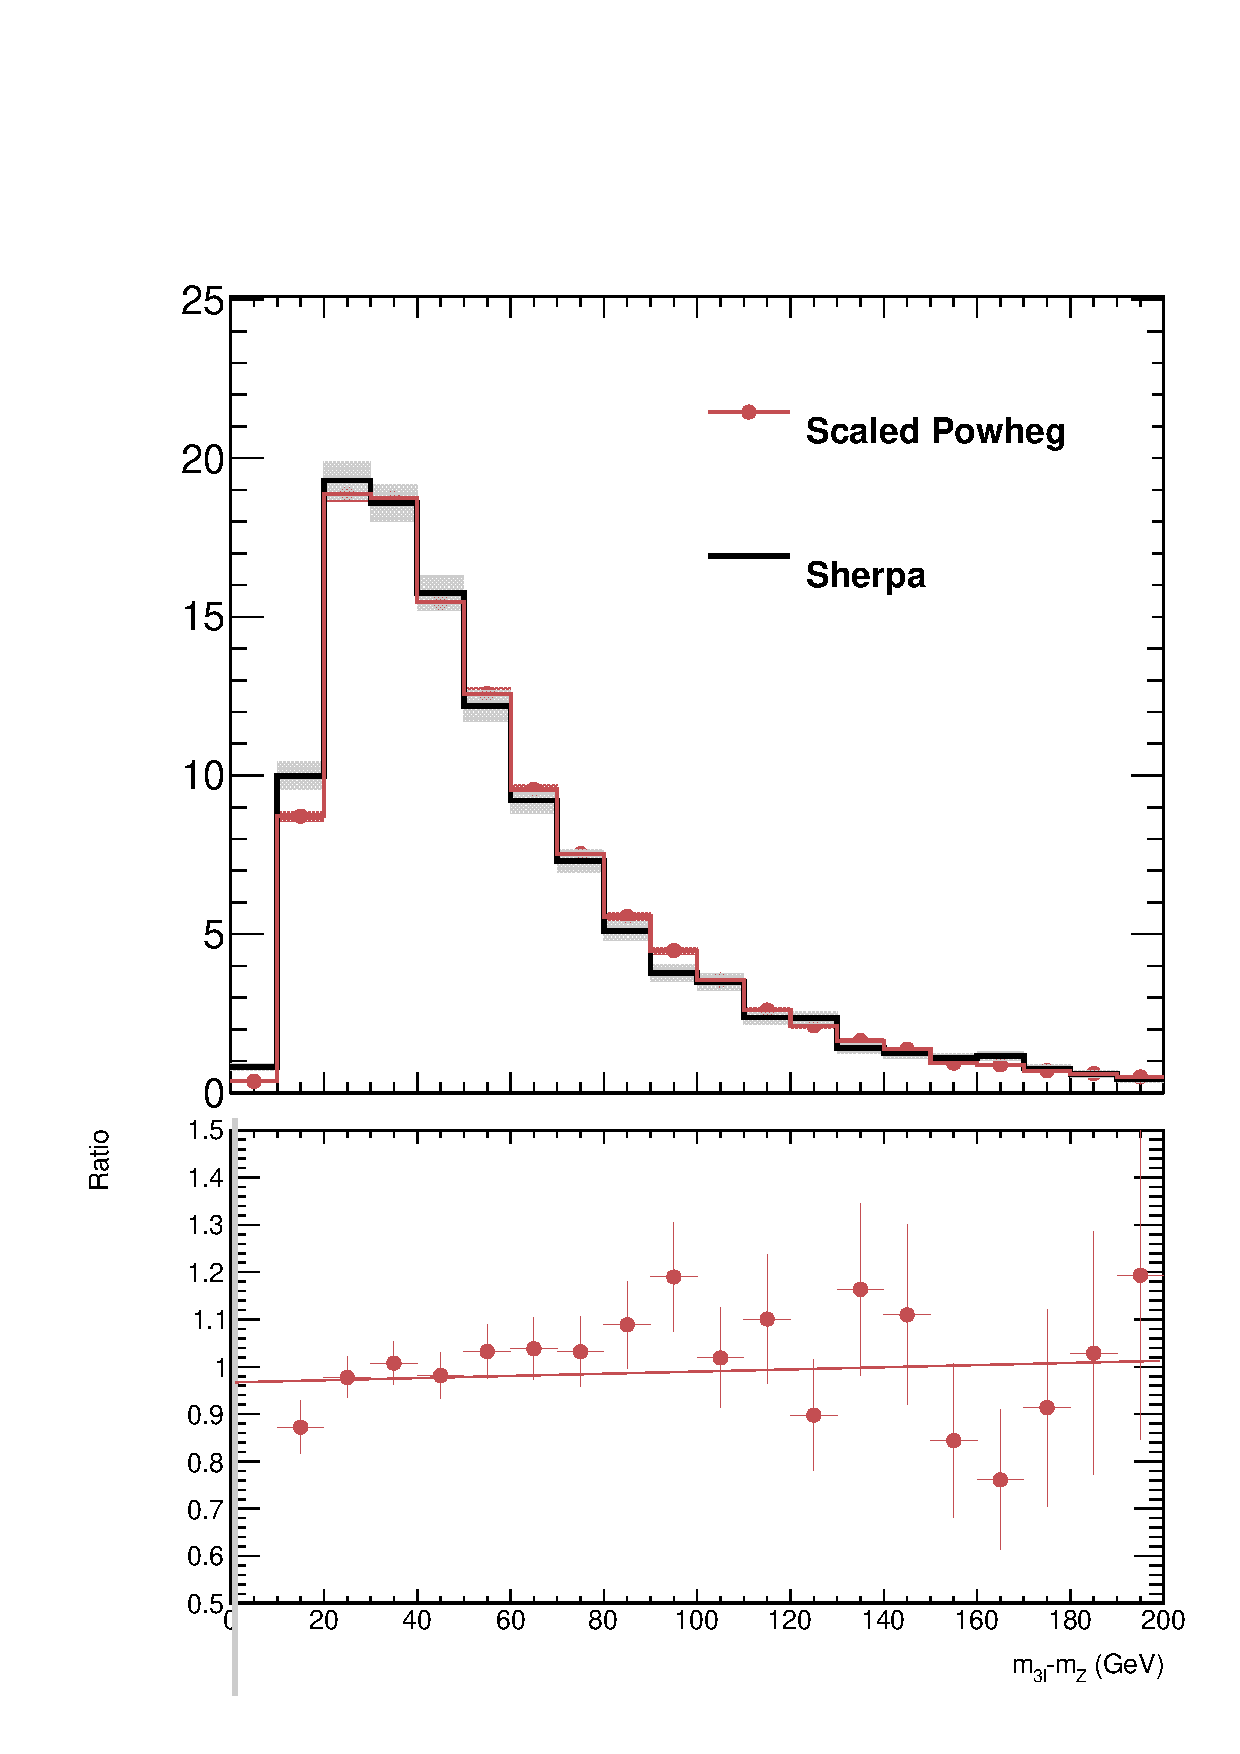
\includegraphics{figures/resonance/c_systematics_ZZShapeSyst_Zmu_InclusiveNoM3L.pdf}}
		}
		\subfloat[ $\threeljj$ SR, $Z+\mu$] {
			\resizebox{2.5in}{!}{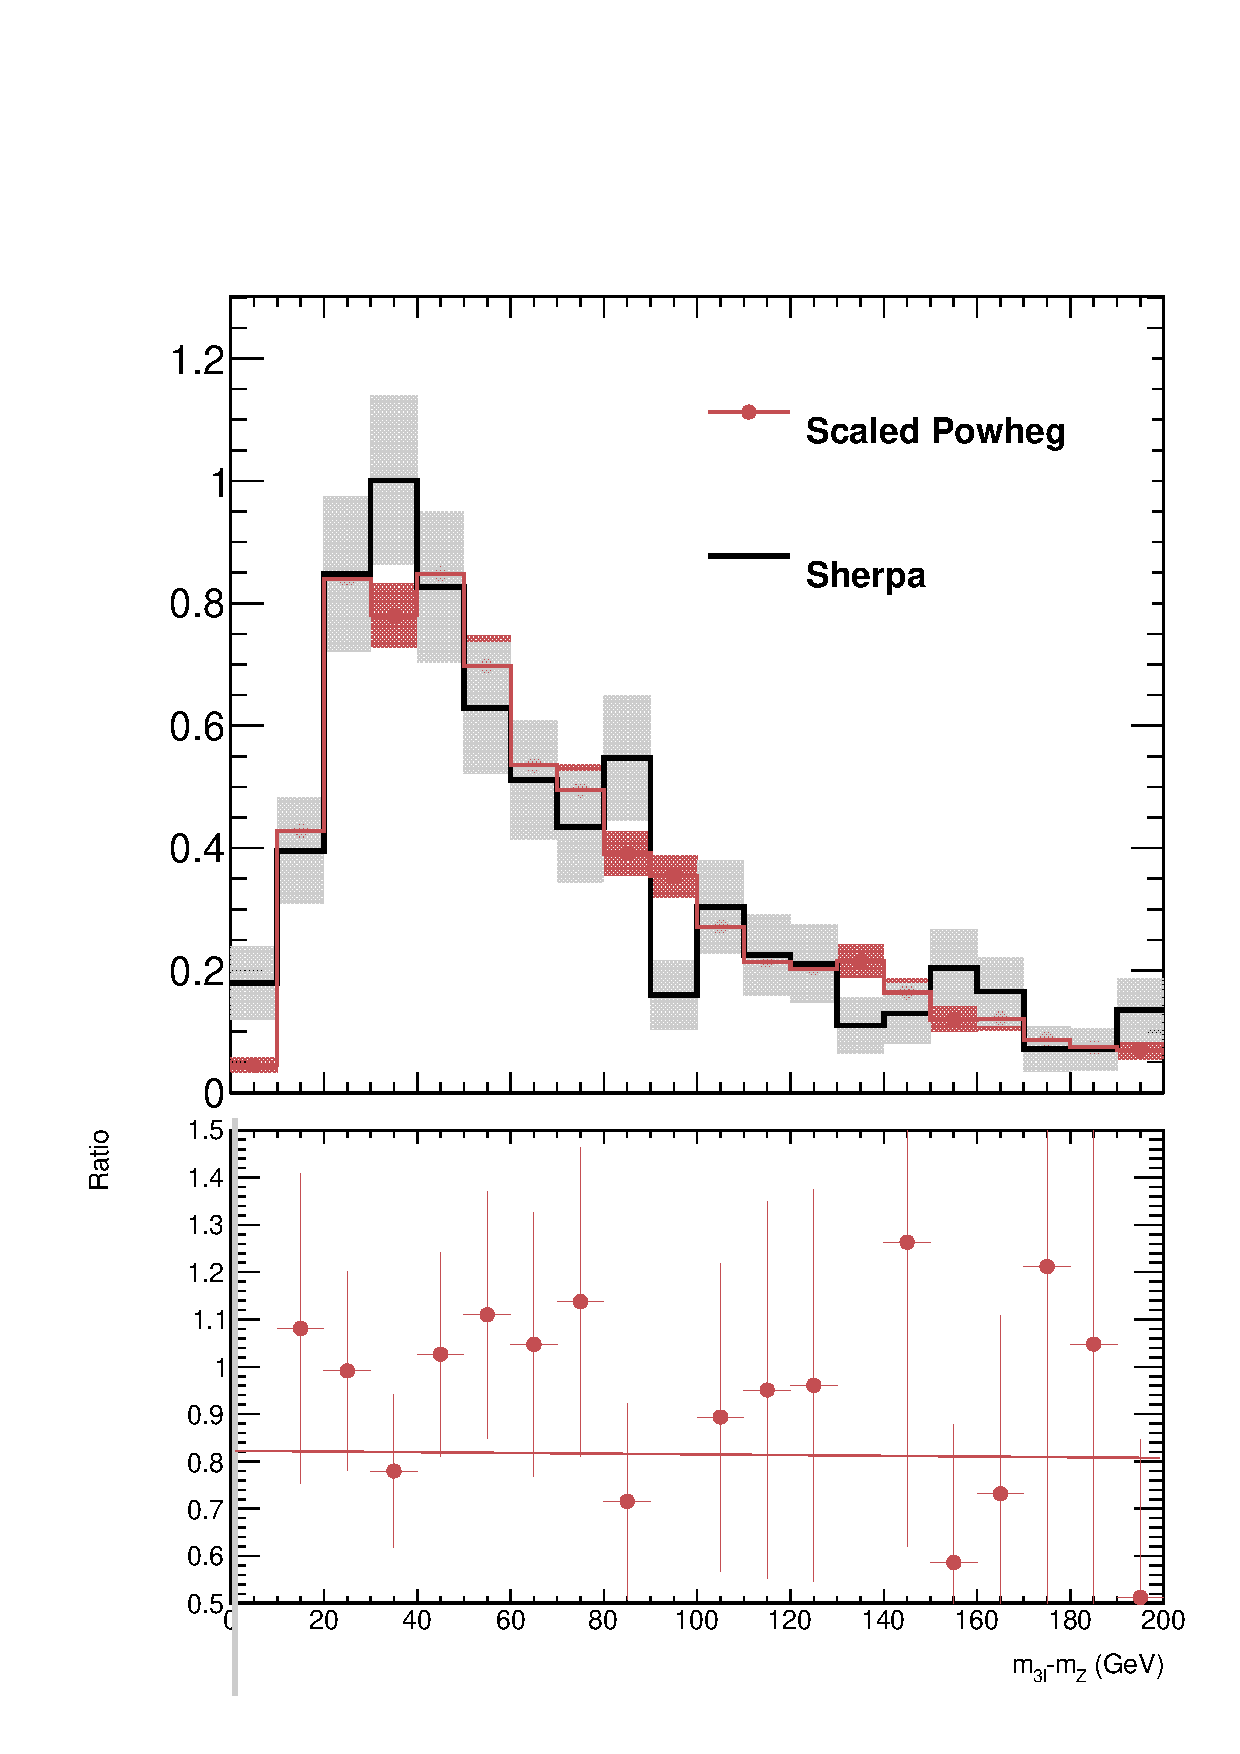
\includegraphics{figures/resonance/c_systematics_ZZShapeSyst_Zmu_ThreeLDijetNoM3L.pdf}}
		}
		\caption{Comparison of the $\deltam$ distributions between \powheg\ and \sherpa\ for the $ZZ$ backgrounds. The \powheg\ events are weighted to account for the mll4 filter.}
		\label{fig:systematic-ZZ-shape}
	\end{figure}
	

	\item \textbf{Monte Carlo statistics and Fit Parameter Uncertainties}: as described below in section~\ref{sec:resonance-fit-method}, the limit setting is performed using fits with analytical functions to the Monte Carlo background predictions. The uncertainty due to the finite statistics of the background samples is in represented in the uncertainties on the fit parameters. This uncertainty is discussed in more detail in section~\ref{sec:fit-limits-systematic-uncertainties}.


	\item \textbf{Monte Carlo sample normalizations}: The Monte Carlo samples used for the irreducible background prediction are normalized to the measured luminosity of the data using theoretical cross sections. The uncertainty on the luminosity is $2.8\%$~\cite{luminosity}. The uncertainties on the cross sections for $WZ$, $ZZ$, and $t\overline{t}+V$ are listed in table~\ref{table:mc-cross-section-uncertainties}. \textcolor{red}{The $WZ$ and $ZZ$ uncertainties are taken from a comparison of \sherpa\ with the NLO generator \vbfnlo.} A cross section uncertainty is not assigned to the $Z+\gamma$ backgrounds; instead, as described next, a large uncertainty is assigned due to applying scale factors to correct the simulated rate of photon conversions. Similarly, an uncertainty is not assigned for the $VVV^{(*)}$ cross section, due to its small contribution to the signal regions. 

	%In the fit-based limit setting procedure, the uncertainty is implemented as a constraint on the normalization of the corresponding sample: the normalizations of the dominant diboson samples are allowed to float within the quadrature sum of all the normalization uncertainties. The normalizations of the small $t\overline{t}+V$ and $VVV^{(*)}$ backgrounds are fixed due to their comparatively small magnitude, which the fit is unable to resolve. 

	\begin{table}[h]
		\centering
		\begin{tabular}{ccc}
			Process & Cross Section Uncertainty & Reference \\
			\hline
			$WZ$ & $7.6\%$ & \cite{DeViveiros:1670929}\\
			$ZZ$ & $4.3\%$ & \cite{DeViveiros:1670929} \\
			$t\overline{t}+V$ & $22\%$ & \cite{ttV} \\
		\end{tabular}	
		\caption{Cross sections and uncertainties for the Monte Carlo samples used for irreducible background estimation.}
		\label{table:mc-cross-section-uncertainties}
	\end{table}

	\item \textbf{Charge flip scale factors}: The rate of trilepton events due to $Z+\gamma$, where the photon converts asymmetrically and is reconstructed as an electron, is observed to be overestimated in Monte Carlo. Scale factors are applied following the charge flip likelihood estimation method from the same-sign dilepton analysis~\cite{DeViveiros:1670929}, and an uncertainty of $30\%$ is assigned to this background sample.

	\item \textbf{Fake factor method}: The systematic uncertainty on the fake factors is described in sections~\ref{sec:electron-fake-factors} and \ref{sec:muon-fake-factors}. They range from $20\%$-$30\%$ for electrons and $25\%$-$50\%$ for muons. 

	\item \textbf{Luminosity}: The uncertainty on the integrated luminosity in 2012 is $2.8\%$. 

	\item \textbf{Lepton scale factors}: Scale factors are applied to equalize the lepton trigger, reconstruction, and identification efficiencies between data and simulation. The corrections are implemented with official performance group tools: 

	\texttt{MuonEfficiencyCorrections}~\cite{MuonEfficiencyScaleFactors} and 

	\texttt{TElectronEfficiencyCorrectionTool}~\cite{ElectronEfficiencyScaleFactors}. 

	Systematic uncertainties on the scale factors are applied according to the official recommendations. 

	\item \textbf{Electron energy corrections}: To improve agreement in electron energy between data and simulation, the energy is scaled in data and smeared in Monte Carlo according to the recommendations at~\cite{ElectronEnergyCorrectionsGEO20,ElectronEnergyCorrectionsGEO21}. The corrections and corresponding systematic uncertainties are provided by the \texttt{ElectronPhotonFourMomentumCorrection} package. 

	\item \textbf{Muon mommentum corrections}: The muon momenta are smeared in simulation according to the recommendations at~\cite{MuonMomentumCorrections}. The corrections are derived by ``comparing the reconstructed muon momentum in experimental and simulated data,'' using $J/\psi$ and $Z$ decays. 

	\item \textbf{Jet energy scale and resolution}: Systematic uncertainties on the jet energy scale and resolution are applied following the recommendations from the Jet/ETMiss group~\cite{JetEtmissRecommendations2012}, and are taken from the package \texttt{JetUncertainties~00-08-07}. The jet energy uncertainties have a small impact on this analysis, only affecting the normalization in the 3L+dijet signal region when the dijet mass is pushed in or out of the window $m_{W}-20~\mbox{GeV}<m_{jj}<m_{h}+25~\mbox{GeV}$. 
\end{itemize}

Figures~\ref{fig:systematics-summary-Ze} and \ref{fig:systematics-summary-Zmu} show the fractional uncertainty due to each source of uncertainty in $20~\mbox{GeV}$ bins for each signal region, as well as the total systematic uncertainty and expected statistical uncertainty. Note that the uncertainties shown are bin-by-bin uncertainties on the Monte Carlo predictions, and do not necessarily correspond to the final uncertainty after fitting the background shapes; for example, after fitting, the Monte Carlo statistical uncertainties are contained in the uncertainties on the fit parameters. Further, the Monte Carlo statistical uncertainties are overrepresented, as they are also contained in the $WZ$/$ZZ$ shape uncertainties derived from the comparison of two statistically independent samples. Finally, due to the fact that the shapes for the 4L and 3L+dijet signal regions are taken from the inclusive signal region, the shape uncertainties derived in these categories are not used in the analysis.

The impact of each uncertainty in each signal region, in terms of fractional uncertainty on the total normalization, is shown for background in figure~\ref{table:systematics-summary}, and some example signal points in figures~\ref{table:systematics-impact-summary-seesaw-160}--\ref{table:systematics-impact-summary-seesaw-500}. The complete set of tables of signal systematics is in appendix~\ref{appx:signal-uncertainties}.


\begin{figure}[p]
	\centering
	\subfloat[ Inclusive SR, $Z+e$] {
		\resizebox{0.48\textwidth}{!}{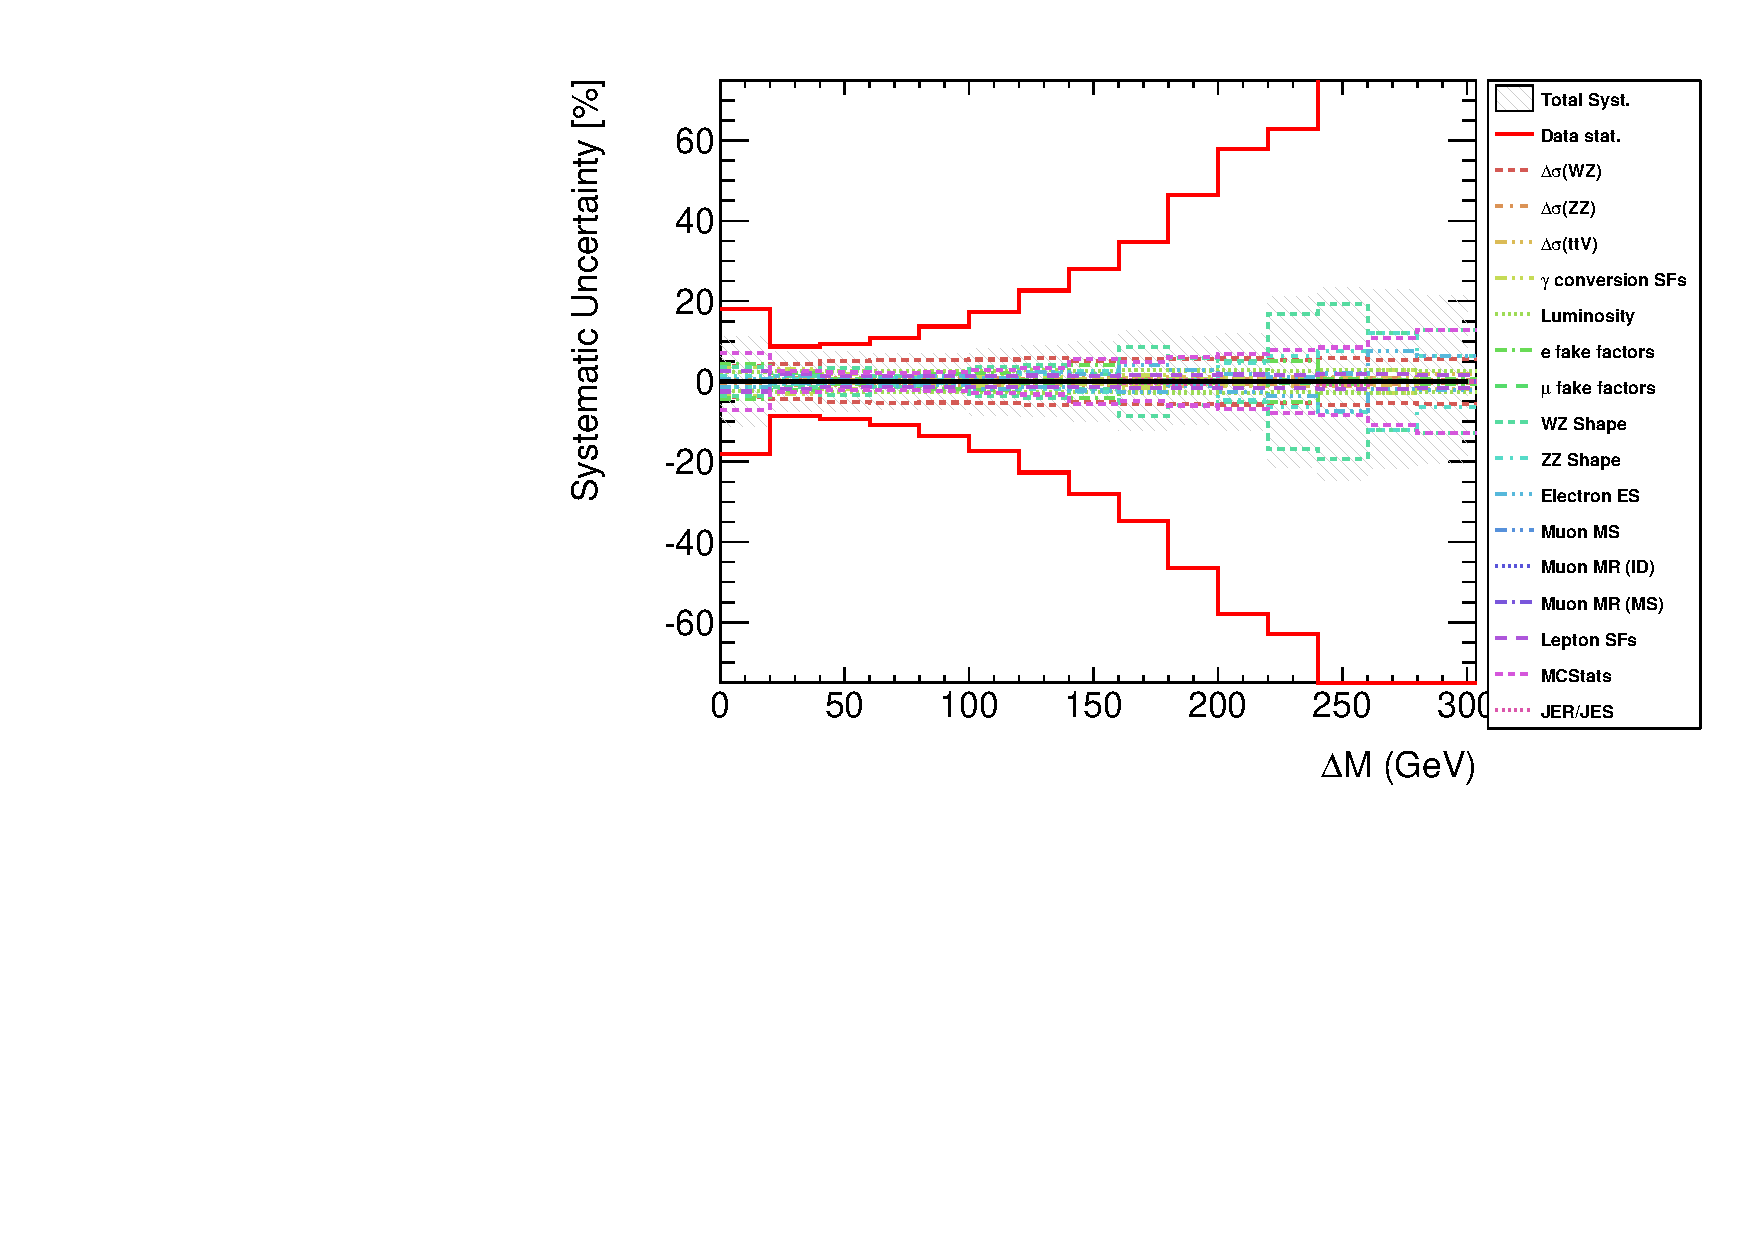
\includegraphics{figures/resonance/c_systematics_DeltaM_Ze_InclusiveNoM3L_300GeV}}
	}
	\subfloat[ 4L SR, $Z+e$] {
		\resizebox{0.48\textwidth}{!}{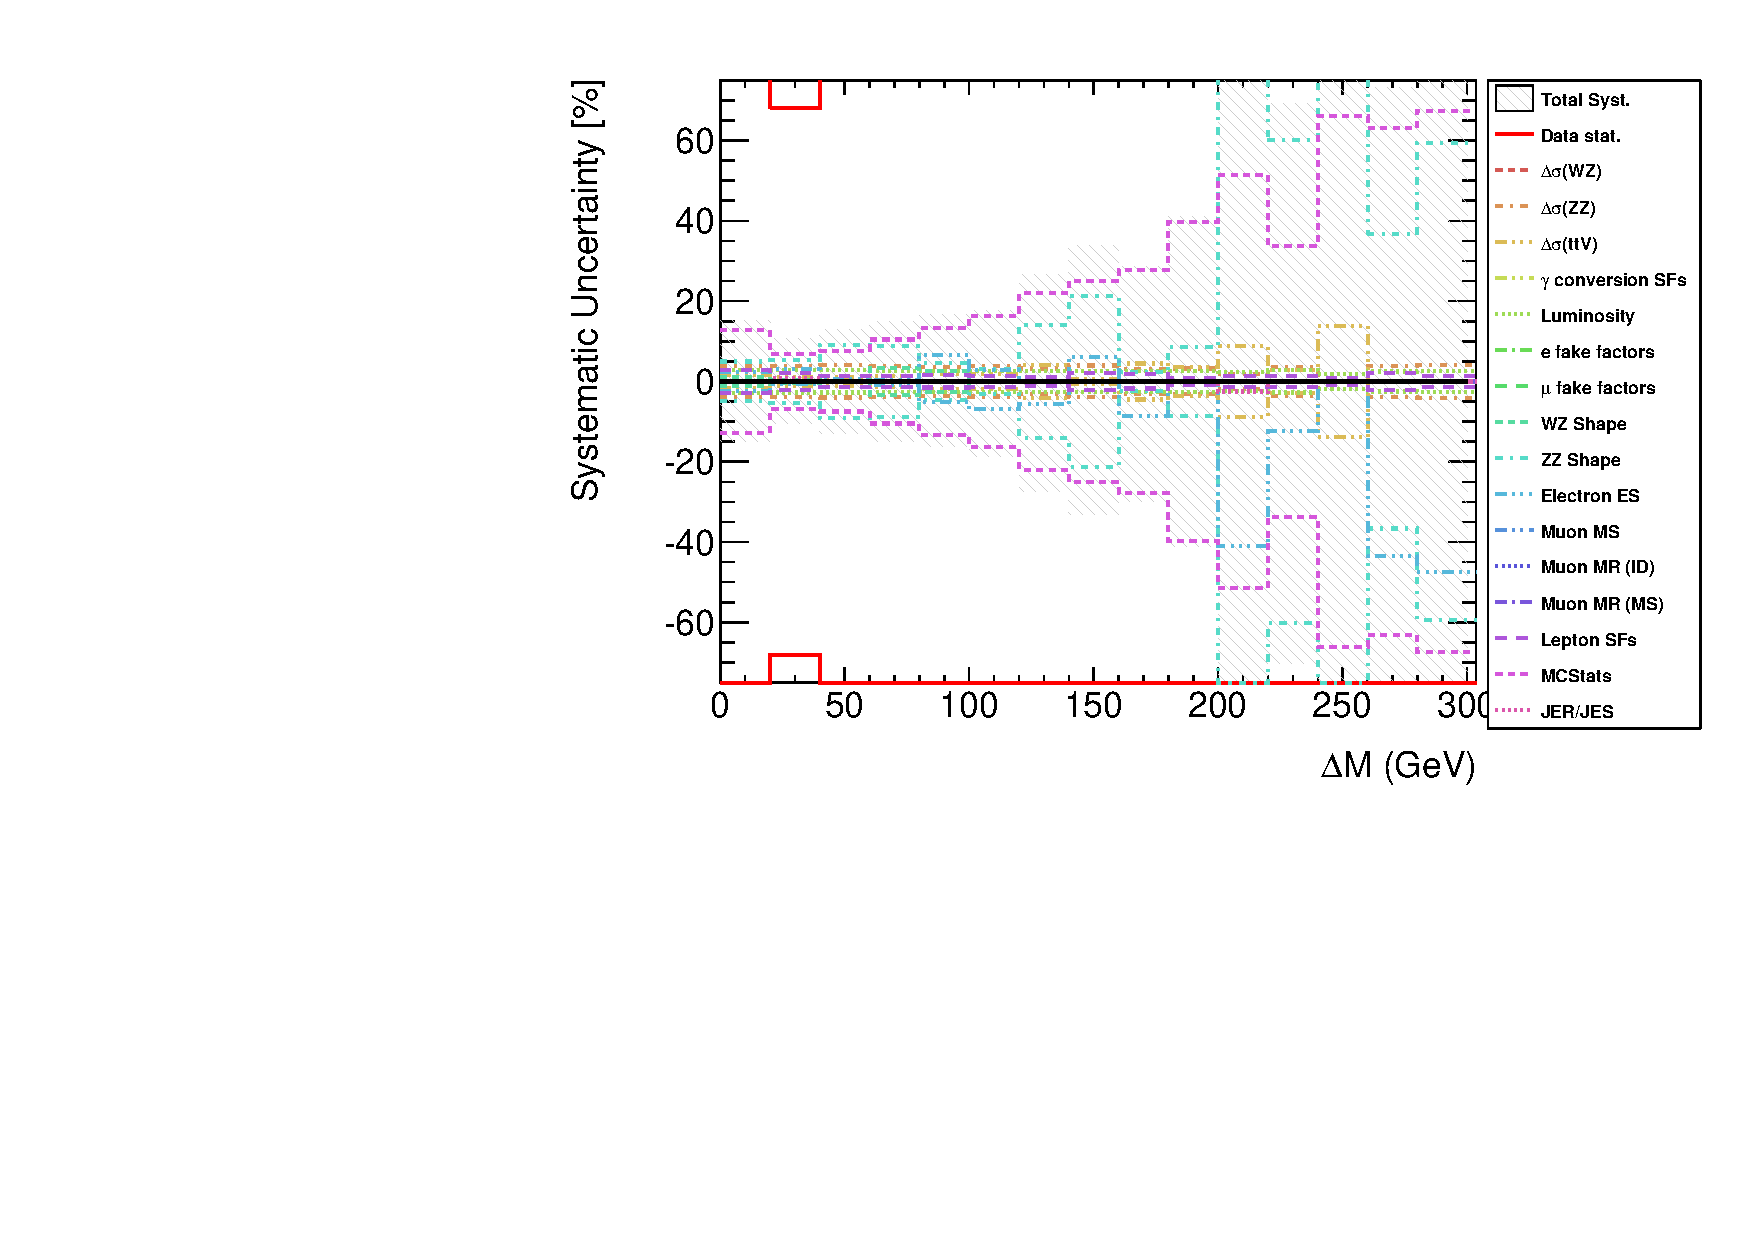
\includegraphics{figures/resonance/c_systematics_DeltaM_Ze_FourLNoM3L_300GeV}}
	} \\
	\subfloat[ 3L+dijet SR, $Z+e$] {
		\resizebox{0.48\textwidth}{!}{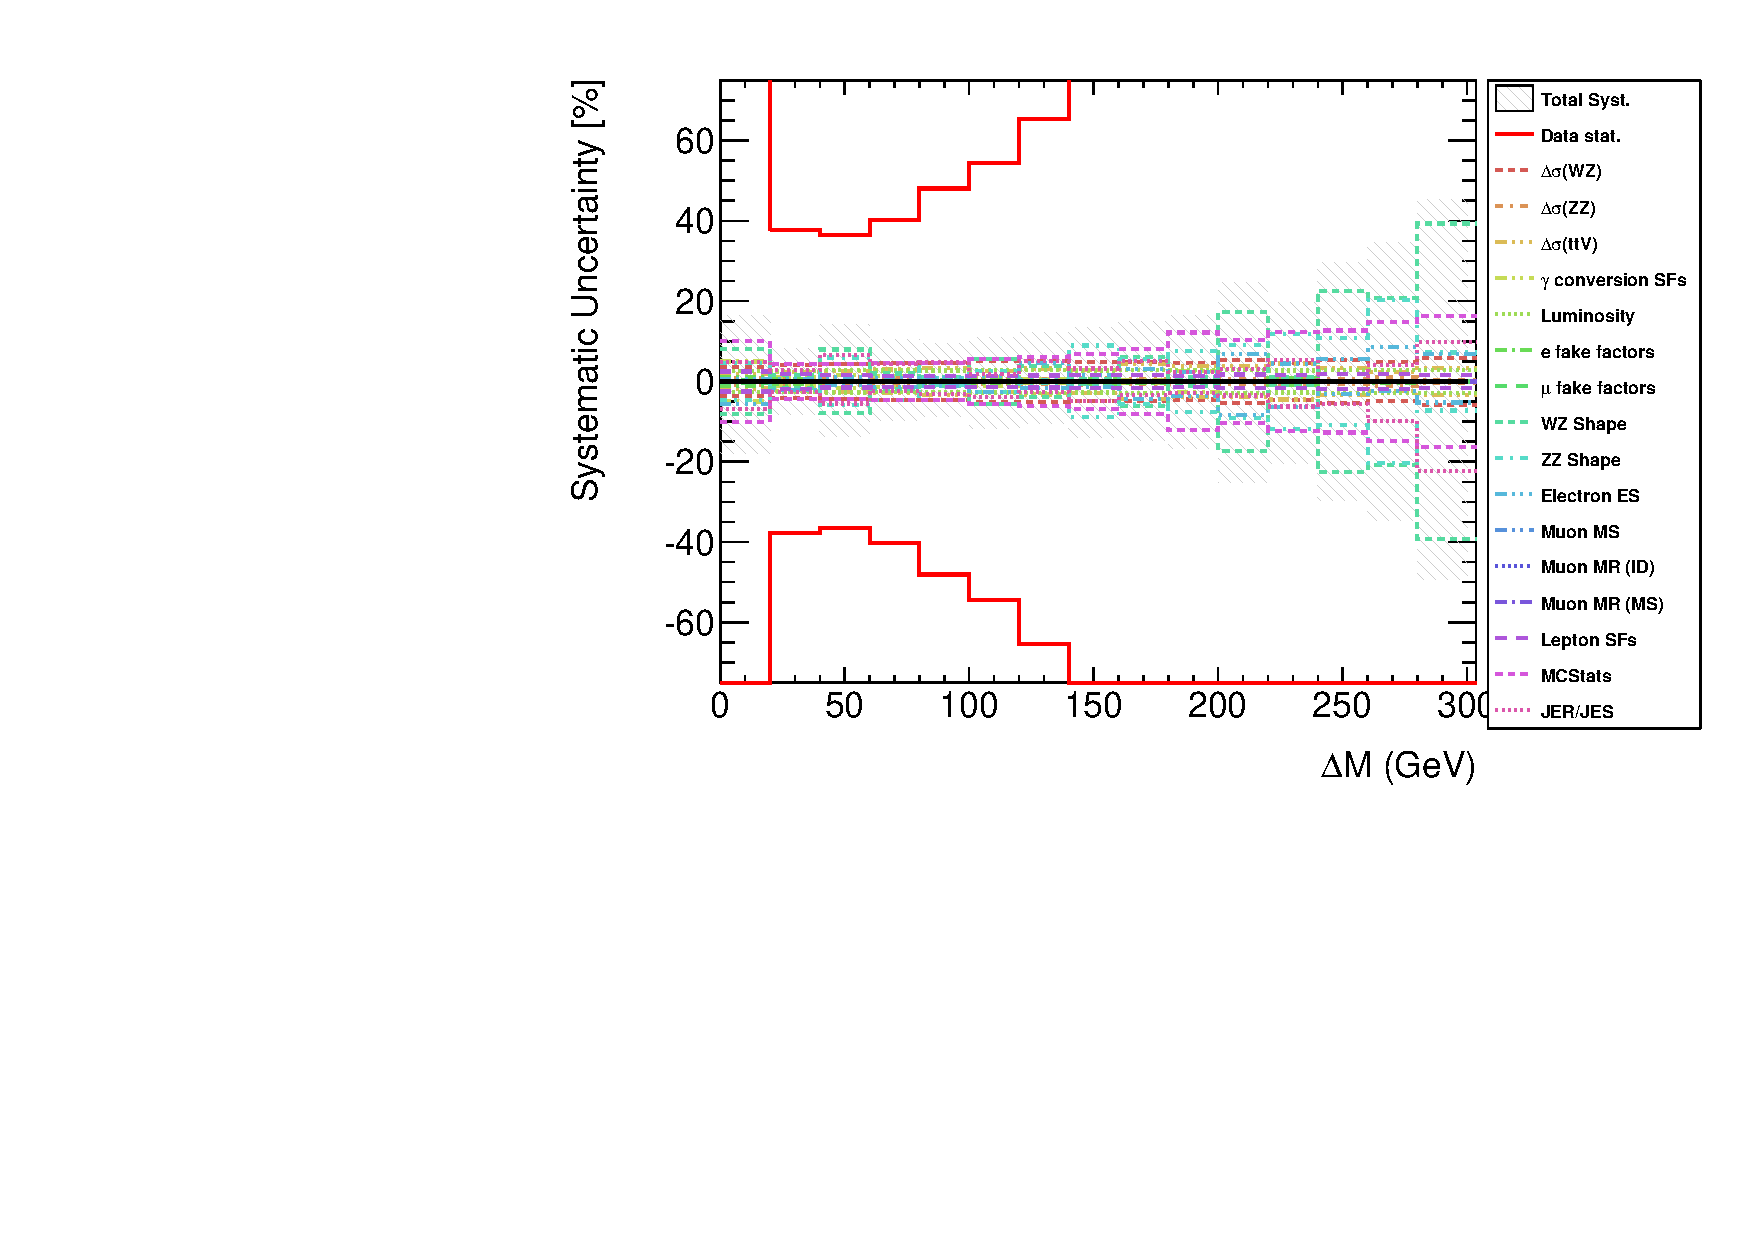
\includegraphics{figures/resonance/c_systematics_DeltaM_Ze_ThreeLDijetNoM3L_300GeV}}
	}
	\subfloat[ Rest SR, $Z+e$] {
		\resizebox{0.48\textwidth}{!}{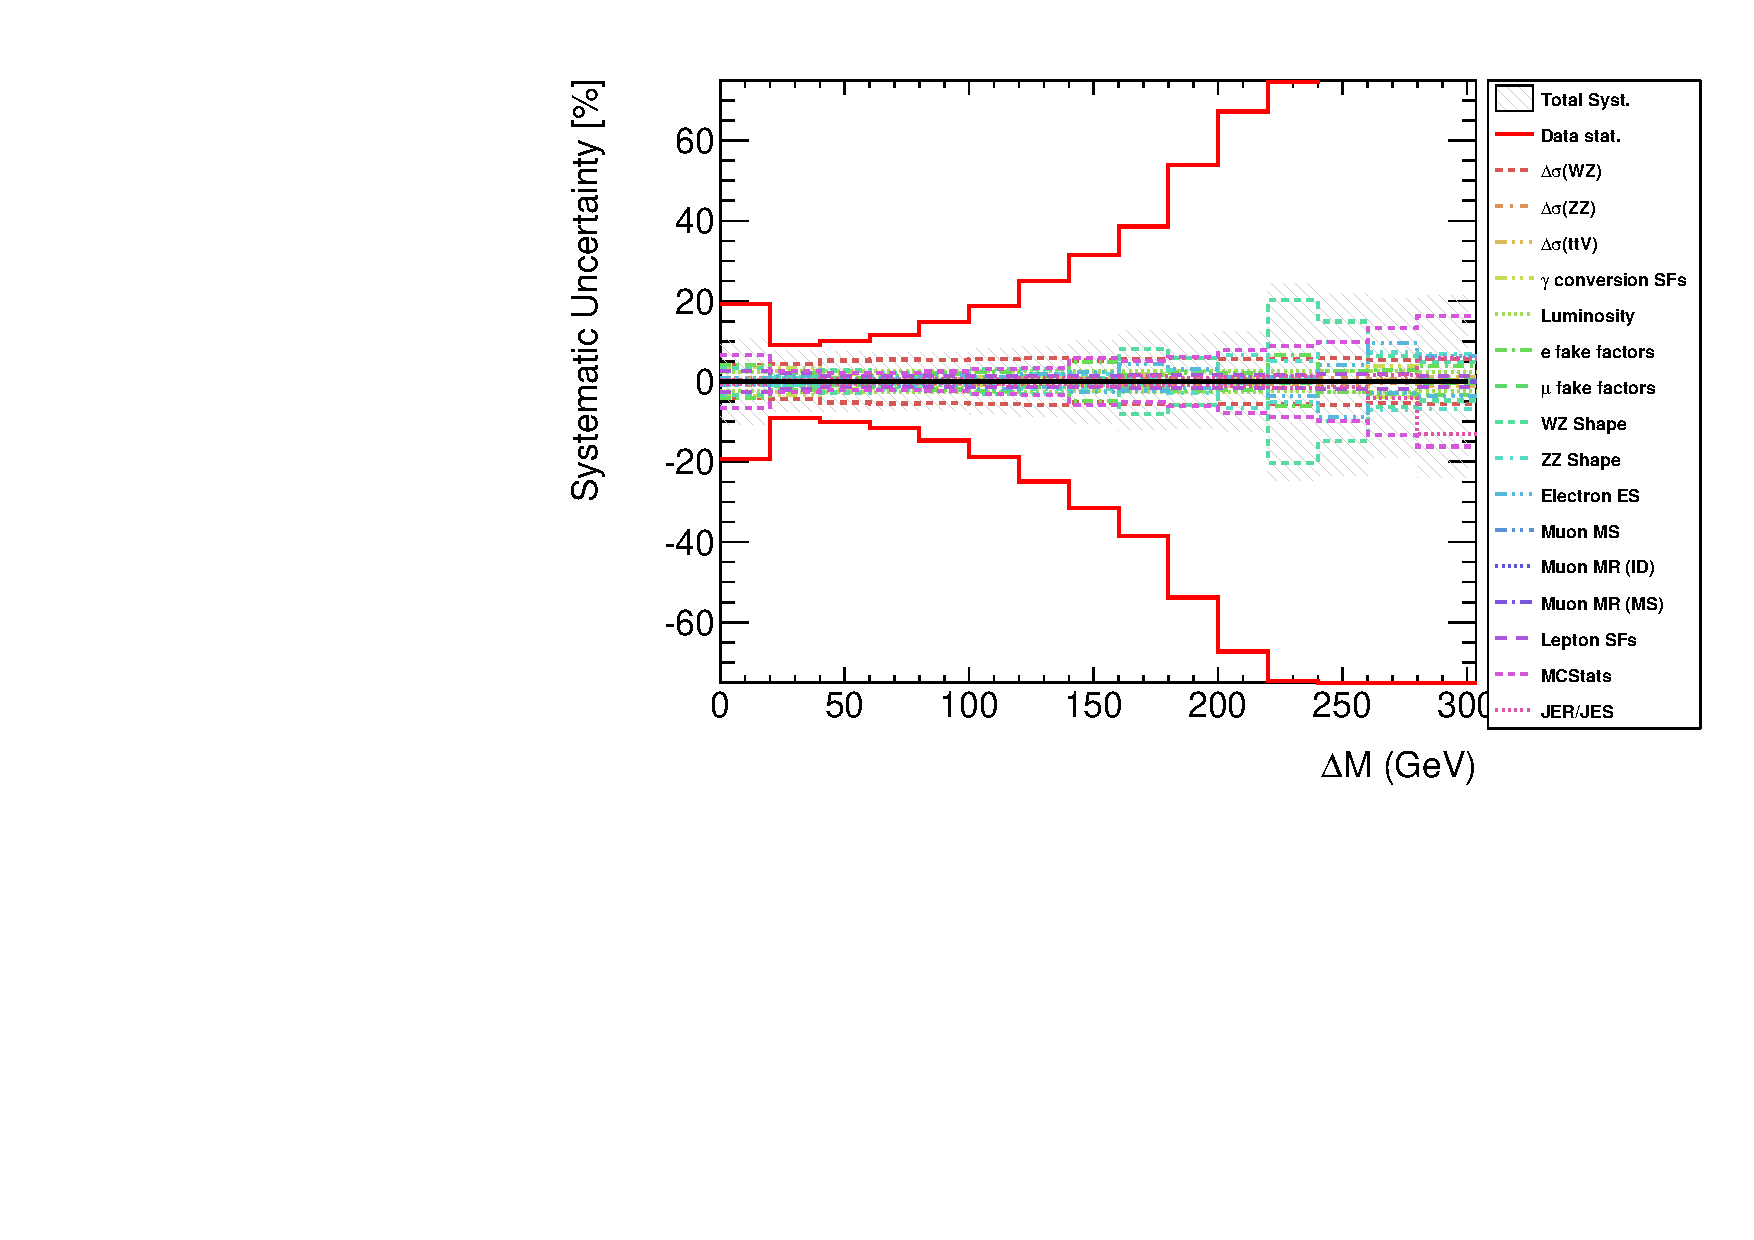
\includegraphics{figures/resonance/c_systematics_DeltaM_Ze_ElseNoM3L_300GeV}}
	}
	\caption{Systematics summary plots for each signal region in the $Z+e$ flavor channel. The contribution from each source of systematic uncertainty is shown in $20~\mbox{GeV}$ bins, along with the total systematic uncertainty and the expected statistical uncertainty. Note that these uncertainties reflect bin-by-bin uncertainties on the Monte Carlo predictions, and do not necessarily correspond to the final uncertainty after fitting the background shapes.}
	\label{fig:systematics-summary-Ze}
\end{figure}

\begin{figure}[p]
	\centering
	\subfloat[ Inclusive SR, $Z+e$] {
		\resizebox{0.48\textwidth}{!}{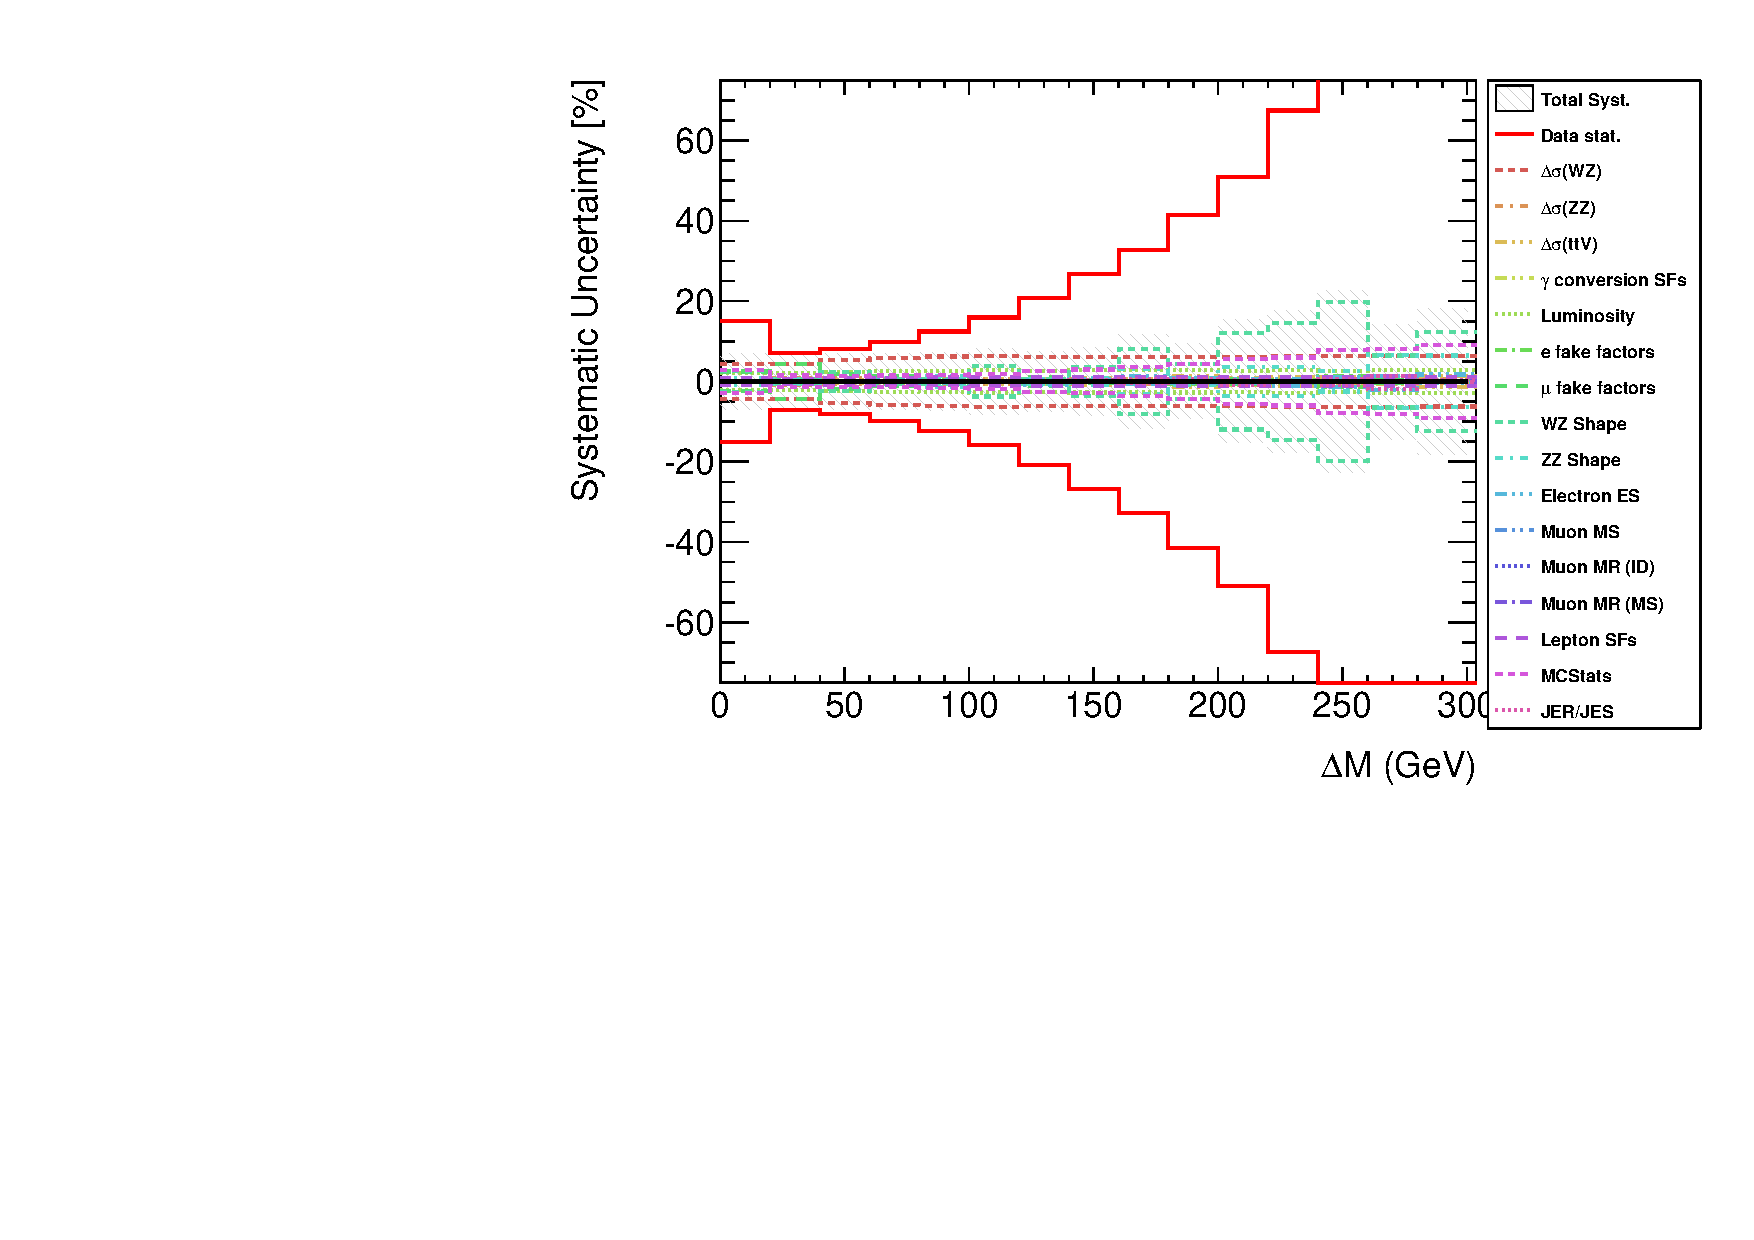
\includegraphics{figures/resonance/c_systematics_DeltaM_Zmu_InclusiveNoM3L_300GeV}}
	}
	\subfloat[ 4L SR, $Z+e$] {
		\resizebox{0.48\textwidth}{!}{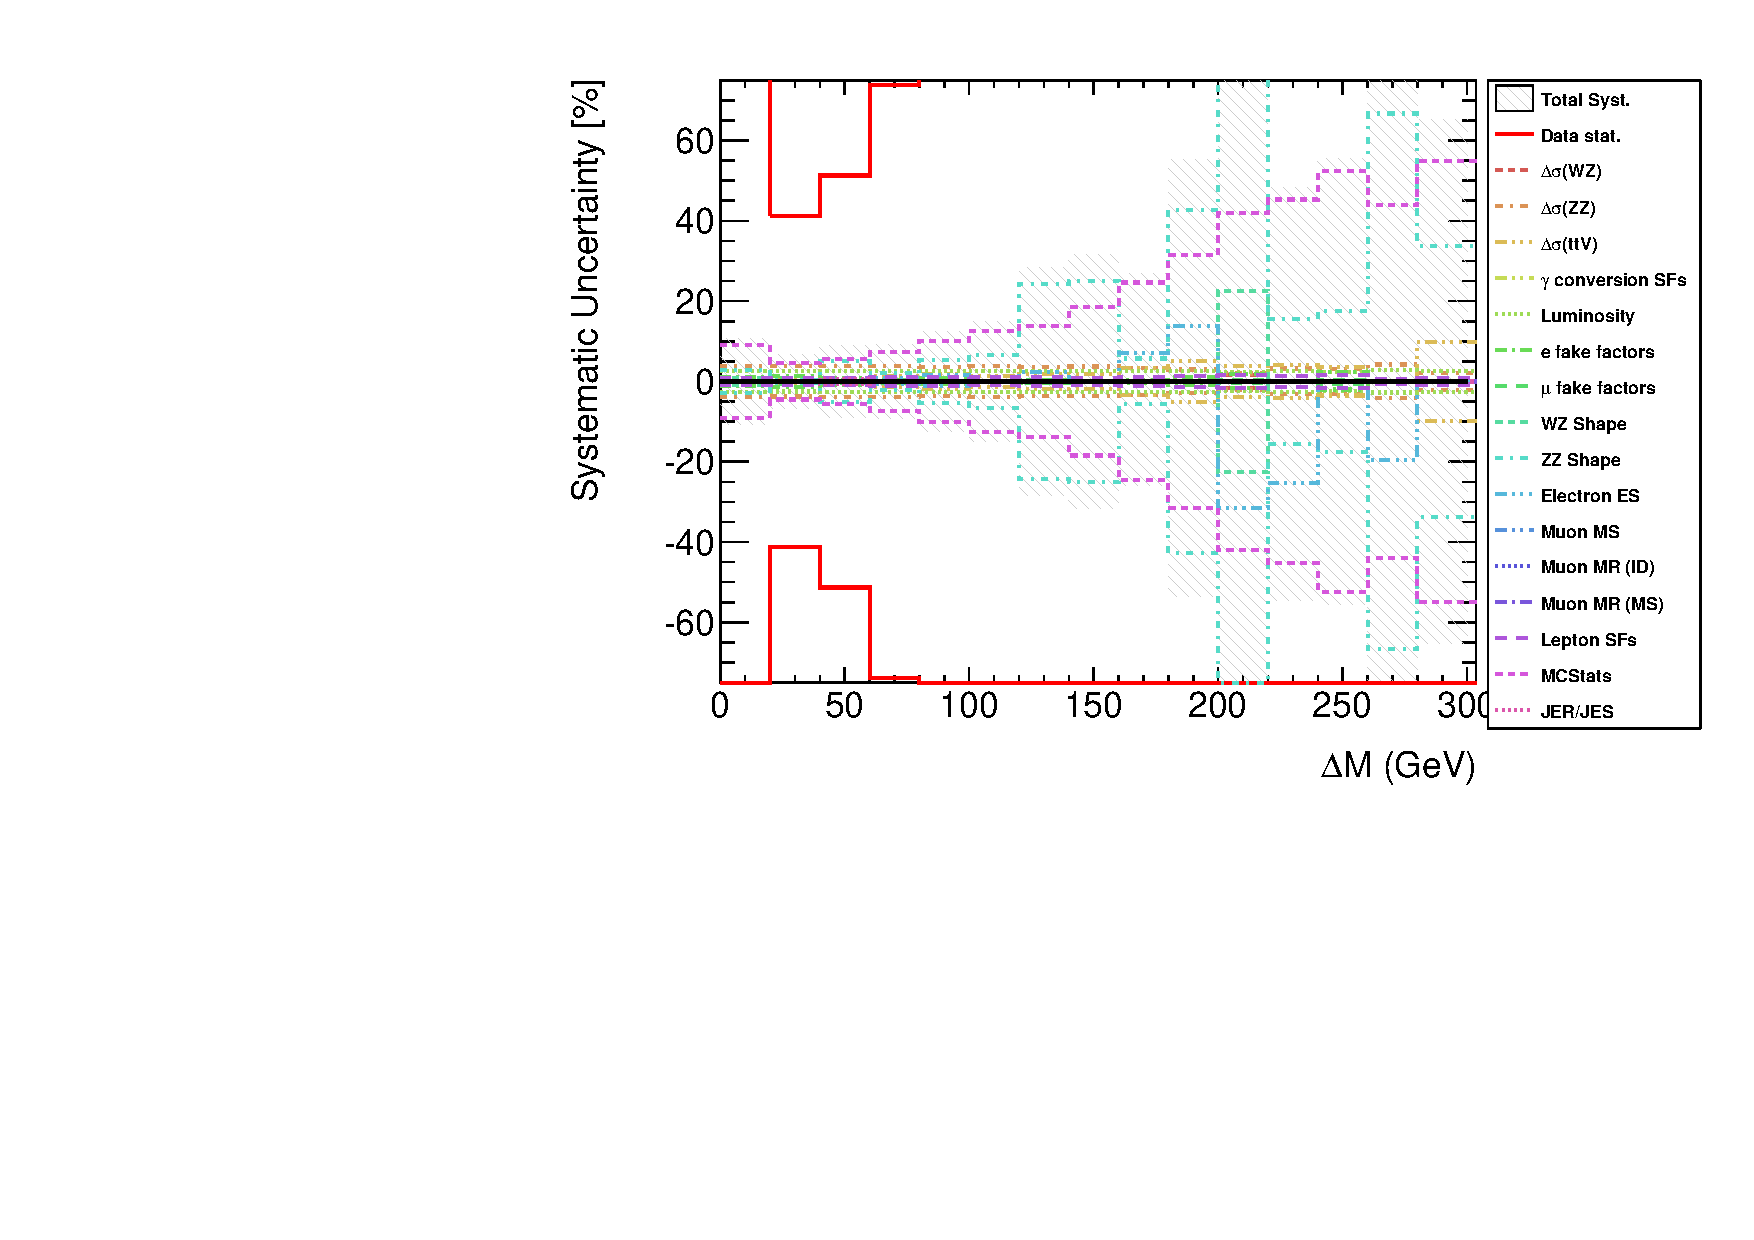
\includegraphics{figures/resonance/c_systematics_DeltaM_Zmu_FourLNoM3L_300GeV}}
	} \\
	\subfloat[ 3L+dijet SR, $Z+e$] {
		\resizebox{0.48\textwidth}{!}{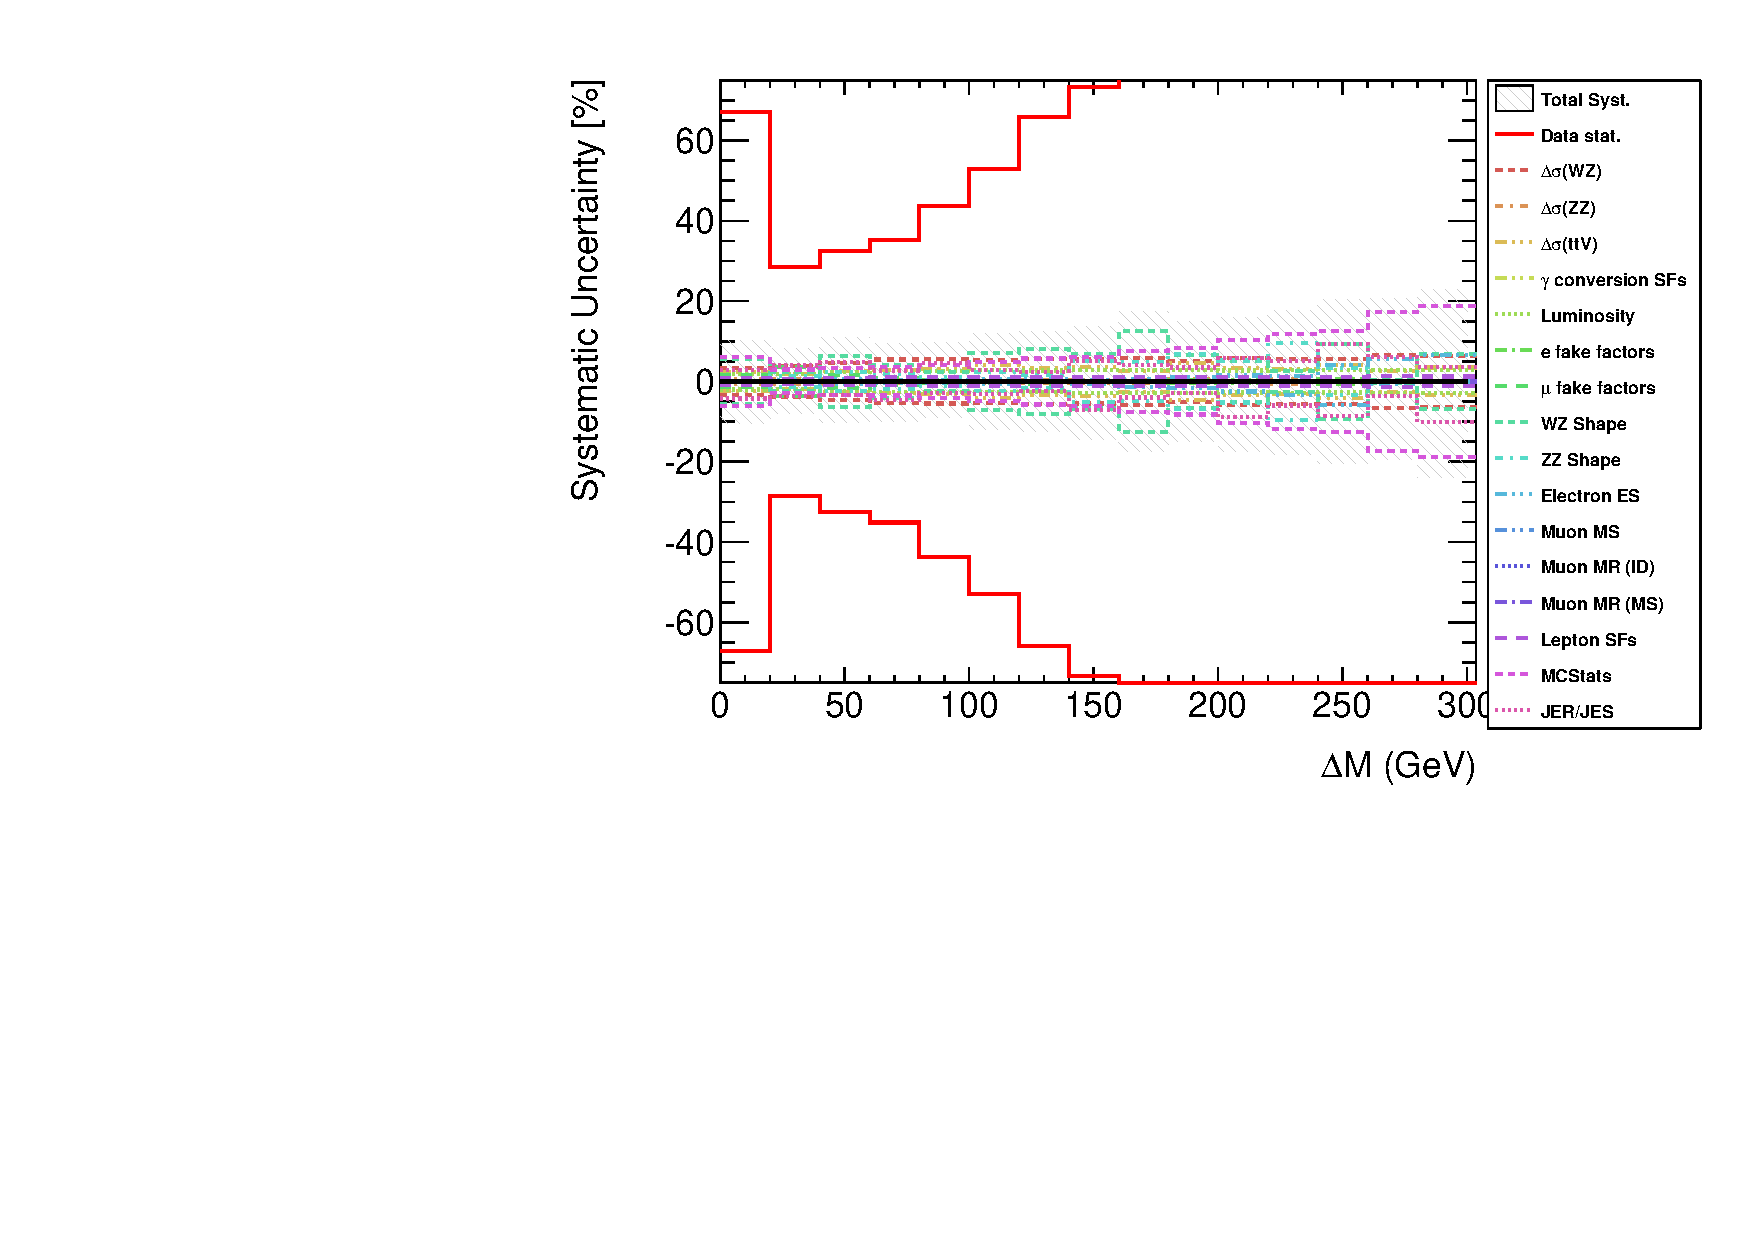
\includegraphics{figures/resonance/c_systematics_DeltaM_Zmu_ThreeLDijetNoM3L_300GeV}}
	}
	\subfloat[ Rest SR, $Z+e$] {
		\resizebox{0.48\textwidth}{!}{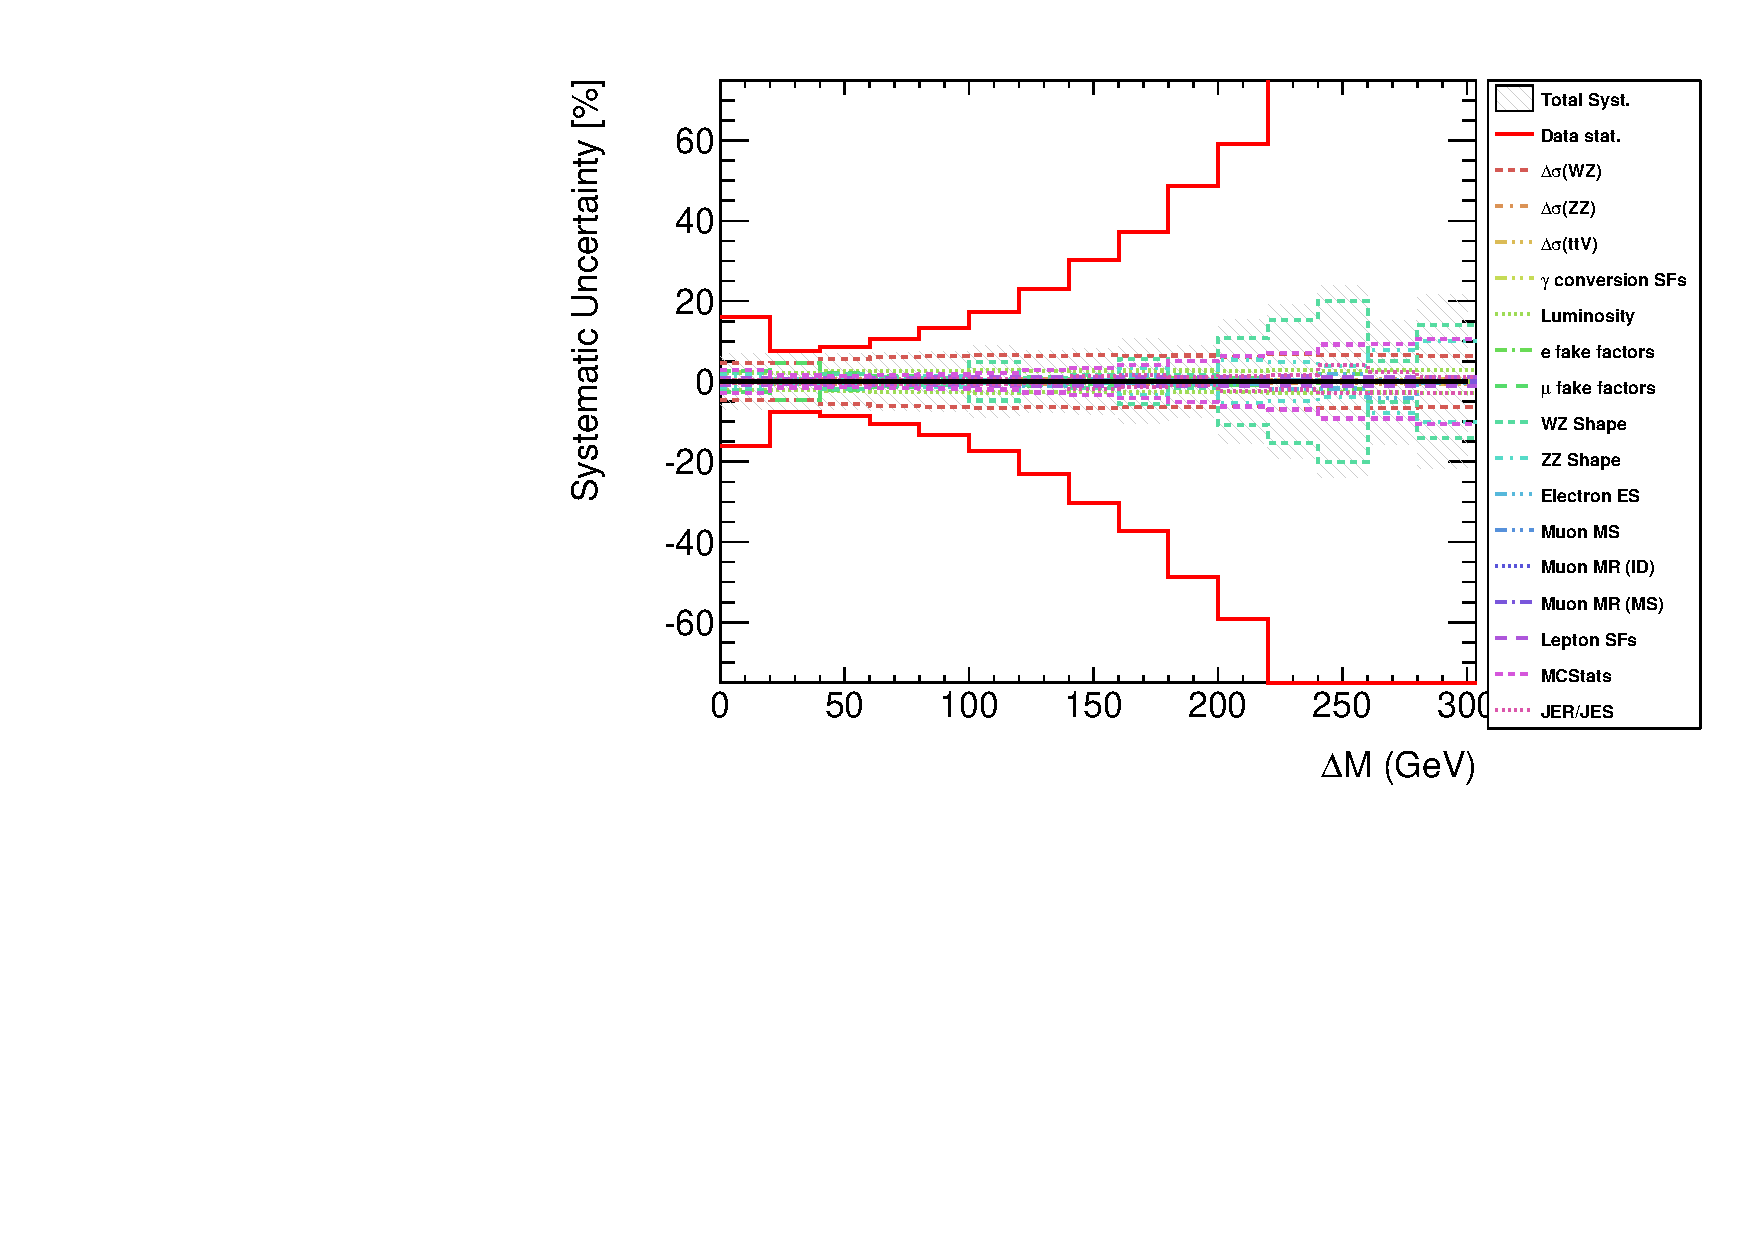
\includegraphics{figures/resonance/c_systematics_DeltaM_Zmu_ElseNoM3L_300GeV}}
	}
	\caption{Systematics summary plots for each signal region in the $Z+\mu$ flavor channel. The contribution from each source of systematic uncertainty is shown in $20~\mbox{GeV}$ bins, along with the total systematic uncertainty and the expected statistical uncertainty. Note that these uncertainties reflect bin-by-bin uncertainties on the Monte Carlo predictions, and do not necessarily correspond to the final uncertainty after fitting the background shapes.}
	\label{fig:systematics-summary-Zmu}
\end{figure}


\begin{table}[htbp]
  \renewcommand{\arraystretch}{1.5}
  \centering
  \begin{tabular}{|c|c|c|c|c||c|c|c|c|}
    \hline
     & \multicolumn{4}{c||}{$Z+e$} & \multicolumn{4}{c|}{$Z+\mu$} \\
    \hline
     &  Total & $4l$ SR & $3l+jj$ SR  & $3l$-only SR  & Total & $4l$ SR & $3l+jj$ SR  & $3l$-only SR  \\
    \hline
    $\sigma_{ZZ}$ & $0.9$  & $3.9$  & $0.9$  & $0.8$  & $0.7$  & $3.8$  & $0.4$  & $0.6$ \\
    $\sigma_{WZ}$ & $4.9$  & $0.1$  & $4.6$  & $5.1$  & $5.3$  & $-$  & $4.9$  & $5.6$  \\
    $\sigma_{ttV}$  & $0.4$  & $1.5$  & $2.9$  & $0.1$  & $0.4$  & $0.9$ & $2.9$  & $0.1$  \\
    Luminosity  & $2.6$ & $2.8$  & $2.7$  & $2.6$  & $2.5$  & $2.6$  & $2.4$  & $2.5$  \\
    $\gamma$ conv. SFs  & $2.0$  & $-$ & $1.2$  & $2.1$  & $-$ & $-$ & $-$ & $-$ \\
    $\ell$ efficiency & $1.6$  & $1.8$  & $1.6$  & $1.6$  & $0.9$  & $0.9$  & $1.0$  & $0.9$  \\
    $e$ reducible SFs  & $1.7$  & $-$ & $0.5$  & $1.9$ & $0.1$ & $0.9$  & $0.1$  & $0.1$  \\
    $\mu$ reducible SFs  &  $0.3$ & $-$ & $0.3$ & $0.3$ & $3.4$ & $0.6$ & $4.3$ & $3.5$  \\
    JES/JER & $0.1$  & $_{-0.0}^{+0.2}$  & $3.3$  & $0.4$  & $0.1$  & $0.2$  & $3.2$  & $0.5$  \\
    LES/LER & $0.6$ & $_{-0.3}^{+1.0}$  & $_{-1.2}^{+0.3}$  & $_{-0.4}^{+0.7}$  & $0.1$  & $0.1$  & $0.2$  & $0.1$  \\
    MC Statistics & $2.4$ & $5.0$ & $4.3$ & $2.6$ & $1.2$ & $3.5$ & $2.8$ & $1.2$ \\
    \hline
    \hline
    Total & $6.9$ & $7.4$ & $8.4$ & $7.1$ & $7.0$ & $6.0$ & $8.7$ & $7.2$ \\
    % Old: wrong muon FFs. 
    % Total & $_{-7.21}^{+7.55}$  & $_{-5.29}^{+5.38}$  & $_{-7.79}^{+8.59}$  & $_{-7.47}^{+7.87}$  & $_{-6.06}^{+6.06}$  & $_{-4.83}^{+4.83}$  & $_{-6.65}^{+7.15}$  & $_{-6.26}^{+6.27}$  \\
    \hline
  \end{tabular}
  \caption{The impact of significant sources of uncertainty on the background prediction in each signal region, in terms of percent of the total background normalization.}
  \label{table:systematics-summary}
\end{table}

\begin{table}[htbp]
  \centering
  \begin{tabular}{|c|c|c|c|c||c|c|c|c|}
    \hline
     & \multicolumn{4}{|c||}{$Z+e$} & \multicolumn{4}{c|}{$Z+\mu$} \\
    \hline
     &  Incl SR & $4l$ SR & $3l+jj$ SR  & $3l$-only SR  & Incl SR & $4l$ SR & $3l+jj$ SR  & $3l$-only SR  \\
    \hline
    Luminosity  & $2.8$ & $2.8$ & $2.8$ & $2.8$ & $2.8$ & $2.8$ & $2.8$ & $2.8$ \\
    $l$ scale factors & $1.7$ & $1.7$ & $1.7$ & $1.6$ & $1.1$ & $1.1$ & $1.1$ & $1.0$ \\
    MC Statistics & $2.1$ & $4.5$ & $3.7$ & $3.0$ & $1.4$ & $2.7$ & $2.7$ & $2.2$ \\
    JES/JER & $0.0$ & $0.2$ & $3.6$ & $3.0$ & $0.2$ & $0.3$ & $3.0$ & $2.2$ \\
    LES/LER & $0.1$ & $0.4$ & $0.1$ & $0.1$ & $0.1$ & $0.2$ & $0.2$ & $0.2$ \\
    \hline
    \hline
    Total & $3.9$ & $5.6$ & $6.1$ & $5.3$ & $3.3$ & $4.0$ & $5.1$ & $4.3$ \\
    \hline
  \end{tabular}
  \caption{The impact of different sources of systematic uncertainty on the signal prediction for the type~III seesaw model with $m_{\lpm}=160 \GeV$, in terms of percent of the total signal normalization.}
  \label{table:systematics-impact-summary-seesaw-160}
\end{table}

\begin{table}[htbp]
  \centering
  \begin{tabular}{|c|c|c|c|c||c|c|c|c|}
    \hline
     & \multicolumn{4}{|c||}{$Z+e$} & \multicolumn{4}{c|}{$Z+\mu$} \\
    \hline
     &  Incl SR & $4l$ SR & $3l+jj$ SR  & $3l$-only SR  & Incl SR & $4l$ SR & $3l+jj$ SR  & $3l$-only SR  \\
    \hline
    Luminosity  & $2.8$ & $2.8$ & $2.8$ & $2.8$ & $2.8$ & $2.8$ & $2.8$ & $2.8$ \\
    $l$ scale factors & $1.8$ & $1.7$ & $1.8$ & $1.9$ & $1.2$ & $1.2$ & $1.2$ & $1.2$ \\
    MC Statistics & $3.0$ & $5.7$ & $4.9$ & $4.7$ & $2.2$ & $3.7$ & $3.8$ & $3.6$ \\
    JES/JER & $0.1$ & $-$ & $1.6$ & $1.7$ & $0.2$ & $0.3$ & $2.0$ & $2.3$ \\
    LES/LER & $0.4$ & $0.1$ & $1.0$ & $0.4$ & $0.3$ & $0.0$ & $0.9$ & $0.3$ \\
    \hline
    \hline
    Total & $4.5$ & $6.5$ & $6.2$ & $6.0$ & $3.8$ & $4.8$ & $5.3$ & $5.3$ \\
    \hline
  \end{tabular}
  \caption{The impact of different sources of systematic uncertainty on the signal prediction for the type~III seesaw model with $m_{\lpm}=300 \GeV$, in terms of percent of the total signal normalization.}
  \label{table:systematics-impact-summary-seesaw-300}
\end{table}

\begin{table}[htbp]
  \centering
  \begin{tabular}{|c|c|c|c|c||c|c|c|c|}
    \hline
     & \multicolumn{4}{|c||}{$Z+e$} & \multicolumn{4}{c|}{$Z+\mu$} \\
    \hline
     &  Incl SR & $4l$ SR & $3l+jj$ SR  & $3l$-only SR  & Incl SR & $4l$ SR & $3l+jj$ SR  & $3l$-only SR  \\
    \hline
    Luminosity  & $2.8$ & $2.8$ & $2.8$ & $2.8$ & $2.8$ & $2.8$ & $2.8$ & $2.8$ \\
    $l$ scale factors & $1.8$ & $1.8$ & $1.8$ & $2.0$ & $1.3$ & $1.4$ & $1.3$ & $1.3$ \\
    MC Statistics & $3.0$ & $5.5$ & $4.8$ & $4.8$ & $2.4$ & $4.0$ & $3.9$ & $4.1$ \\
    JES/JER & $-$ & $-$ & $1.7$ & $1.9$ & $0.3$ & $0.5$ & $1.8$ & $2.5$ \\
    LES/LER & $0.4$ & $0.5$ & $2.1$ & $1.7$ & $0.4$ & $1.6$ & $2.8$ & $2.2$ \\
    \hline
    \hline
    Total & $4.5$ & $6.4$ & $6.4$ & $6.4$ & $3.9$ & $5.4$ & $6.0$ & $6.1$ \\
    \hline
  \end{tabular}
  \caption{The impact of different sources of systematic uncertainty on the signal prediction for the type~III seesaw model with $m_{\lpm}=500 \GeV$, in terms of percent of the total signal normalization.}
  \label{table:systematics-impact-summary-seesaw-500}
\end{table}


\section{Background Validation}\label{sec:resonance-background-validation}
For each flavor channel, four validation regions are defined to test the background predictions from the Monte Carlo simulation samples and the fake factor procedure. Each region starts from the set of events with three selected electrons or muons, two of which form an OSSF pair of leptons. 

The \underline{\textbf{high $\Delta R$}} region contains events with large separation between the $Z$ candidate momentum and the off-$Z$ lepton momentum, $\Delta R(Z,\,\ell_3)>3$. Events are also required to have exactly three leptons, and to satify $\deltam<200 \GeV - m_Z$, to limit signal contamination from hypotheses with larger $m_{\lpm}$ where the $Z$ and the off-$Z$ lepton are less collimated. The region has a similar background composition to the signal regions with three leptons, and tests the $WZ$, $ZZ$, and reducible background predictions.

The \underline{\textbf{$ZZ$}} region contains events with two OSSF lepton pairs with invariant mass within $10 \GeV$ of $m_Z$. The region tests the $ZZ$ background prediction.

The \underline{\textbf{off-$Z$}} region contains events with exactly three leptons, with an OSSF pair within $50 \GeV$ of $m_Z$, but no OSSF pairs with invariant mass within $20 \GeV$ of $m_Z$. As the event does not contain a $Z$ candidate, the trilepton selection is modified: the highest mass OSSF pair is selected, and the third lepton is chosen to be the remaining lepton. In the $Z+e$ flavor channel, this region tests the $Z+\gamma$ background prediction. In the $Z+\mu$ channel, the region is dominated by $ZZ$, where one lepton is not selected, and the other two leptons originate from an off-shell $Z^{*}/\gamma^{*}$. 

The \underline{\textbf{$WZ$}} region contains events with exactly three leptons, two of which form an OSSF pair within $10~\mbox{GeV}$ of $m_Z$, and the third of which satisfies $40~\mbox{GeV}<\mtw<90~\mbox{GeV}$. Additionally, the validation region requires $40~\mbox{GeV}<\Etmiss<100~\mbox{GeV}$ and zero jets, which suppresses signal contamination.

The definition of each validation region and the backgrounds tested are summarized in table~\ref{table:resonance-validation-region-definitions}. The total number of observed and predicted events in each region is shown in table~\ref{table:resonance-validation-region-normalizations}, and the corresponding $\deltam$ distributions are shown in figure~\ref{fig:resonance-validation-regions}. Good agreement is seen in most validation regions, with the observed and predicted normalizations agreeing to better than $1.5\sigma$. A deficit of data with respect to the background prediction is seen in the off-$Z$, $Z+\mu$ validation region, corresponding to $2.3\sigma$. The region is dominated by contributions from $ZZ$, where only three leptons pass the selection requirements and no same-flavour, opposite-sign lepton pair is reconstructed with invariant mass within $20 \GeV$ of $m_Z$. 


\begin{table}[htbp]
	\centering
	\resizebox{6in}{!}{
	\begin{tabular}{|c|c|c|}
		\hline
		Control Region & Definition & Background Tested \\
		\hline
		\multirow{2}{*}{High $\Delta R$} & $\Delta R(Z,\,\ell_3)>3.0$ & $WZ$, $ZZ$, and reducible \\
		 & $\deltam < 200~\mbox{GeV} - m_Z$ & \\
		\hline
		Off $Z$ & Reject events with $|m_{ll}-m_Z|<20~\mbox{lGeV}$ & $Z+\gamma$ ($Z+e$ events) and $ZZ$ ($Z+\mu$ events) \\
		\hline
		Two $Z$ & Require 2 $Z$ candidates ($|m_{ll}-m_Z|<10~\mbox{GeV}$) & $ZZ$ \\
		\hline
		\multirow{3}{*}{$WZ$} & $3$ leptons, 0 jets, & $WZ$\\
		 & $40~\mbox{GeV}<\mtw<90~\mbox{GeV}$, & \\
		 & $40~\mbox{GeV}<\Etmiss<100~\mbox{GeV}$ & \\ 
		\hline
	\end{tabular}
	}
	\caption{Definitions and targeted backgrounds of the four validation regions.}
	\label{table:resonance-validation-region-definitions}
\end{table}

\begin{table}[htbp]
	\centering
	\begin{tabular}{|c|c|c|c|c|}
		\hline
		Flavor Channel & Control Region & Data & Background Prediction & $\frac{\mbox{Data}-\mbox{Bkgd}}{\sigma_{\mathrm{bkgd}}}$ \\
		\hline
		$Z+e$	&	High $\Delta R$	&	$239$	&	$239.16 	\pm 15.47^{(\mathrm{stat})} \pm 13.66^{(\mathrm{syst})}$ 	&	-0.01	\\
		\hline
		$Z+e$	&	OffZ		&	$360$	&	$348.81 	\pm 18.68^{(\mathrm{stat})} \pm 44.21^{(\mathrm{syst})}$ 	&	0.23	\\
		\hline
		$Z+e$	&	TwoZ		&	$39	$	&	$37.29 		\pm 6.11^{(\mathrm{stat})} \pm 2.14^{(\mathrm{syst})}$ 		&	0.26	\\
		\hline
		$Z+e$	&	WZ			&	$140$	&	$133.47 	\pm 11.56^{(\mathrm{stat})} \pm 10.29^{(\mathrm{syst})}$ 	&	0.42	\\
		\hline
		$Z+\mu$	&	High $\Delta R$	&	$302$	&	$301.00 	\pm 17.35^{(\mathrm{stat})} \pm 12.33^{(\mathrm{syst})}$ 	&	0.05	\\
		\hline
		$Z+\mu$	&	OffZ		&	$163$	&	$200.25 	\pm 14.16^{(\mathrm{stat})} \pm 7.77^{(\mathrm{syst})}$ 	&	-2.31	\\
		\hline
		$Z+\mu$	&	TwoZ		&	$74	$	&	$63.4 		\pm 7.97^{(\mathrm{stat})} \pm 3.43^{(\mathrm{syst})}$ 		&	1.22	\\
		\hline
		$Z+\mu$	&	WZ			&	$222$	&	$192.96 	\pm 13.90^{(\mathrm{stat})} \pm 14.42^{(\mathrm{syst})}$ 	&	1.45	\\
		\hline
	\end{tabular}
	\caption{Summary of number of events observed and predicted for each control region.}
	\label{table:resonance-validation-region-normalizations}
\end{table}

\begin{figure}[h]
	\centering
	\subfloat[ $Z+e$] {
		\resizebox{3in}{!}{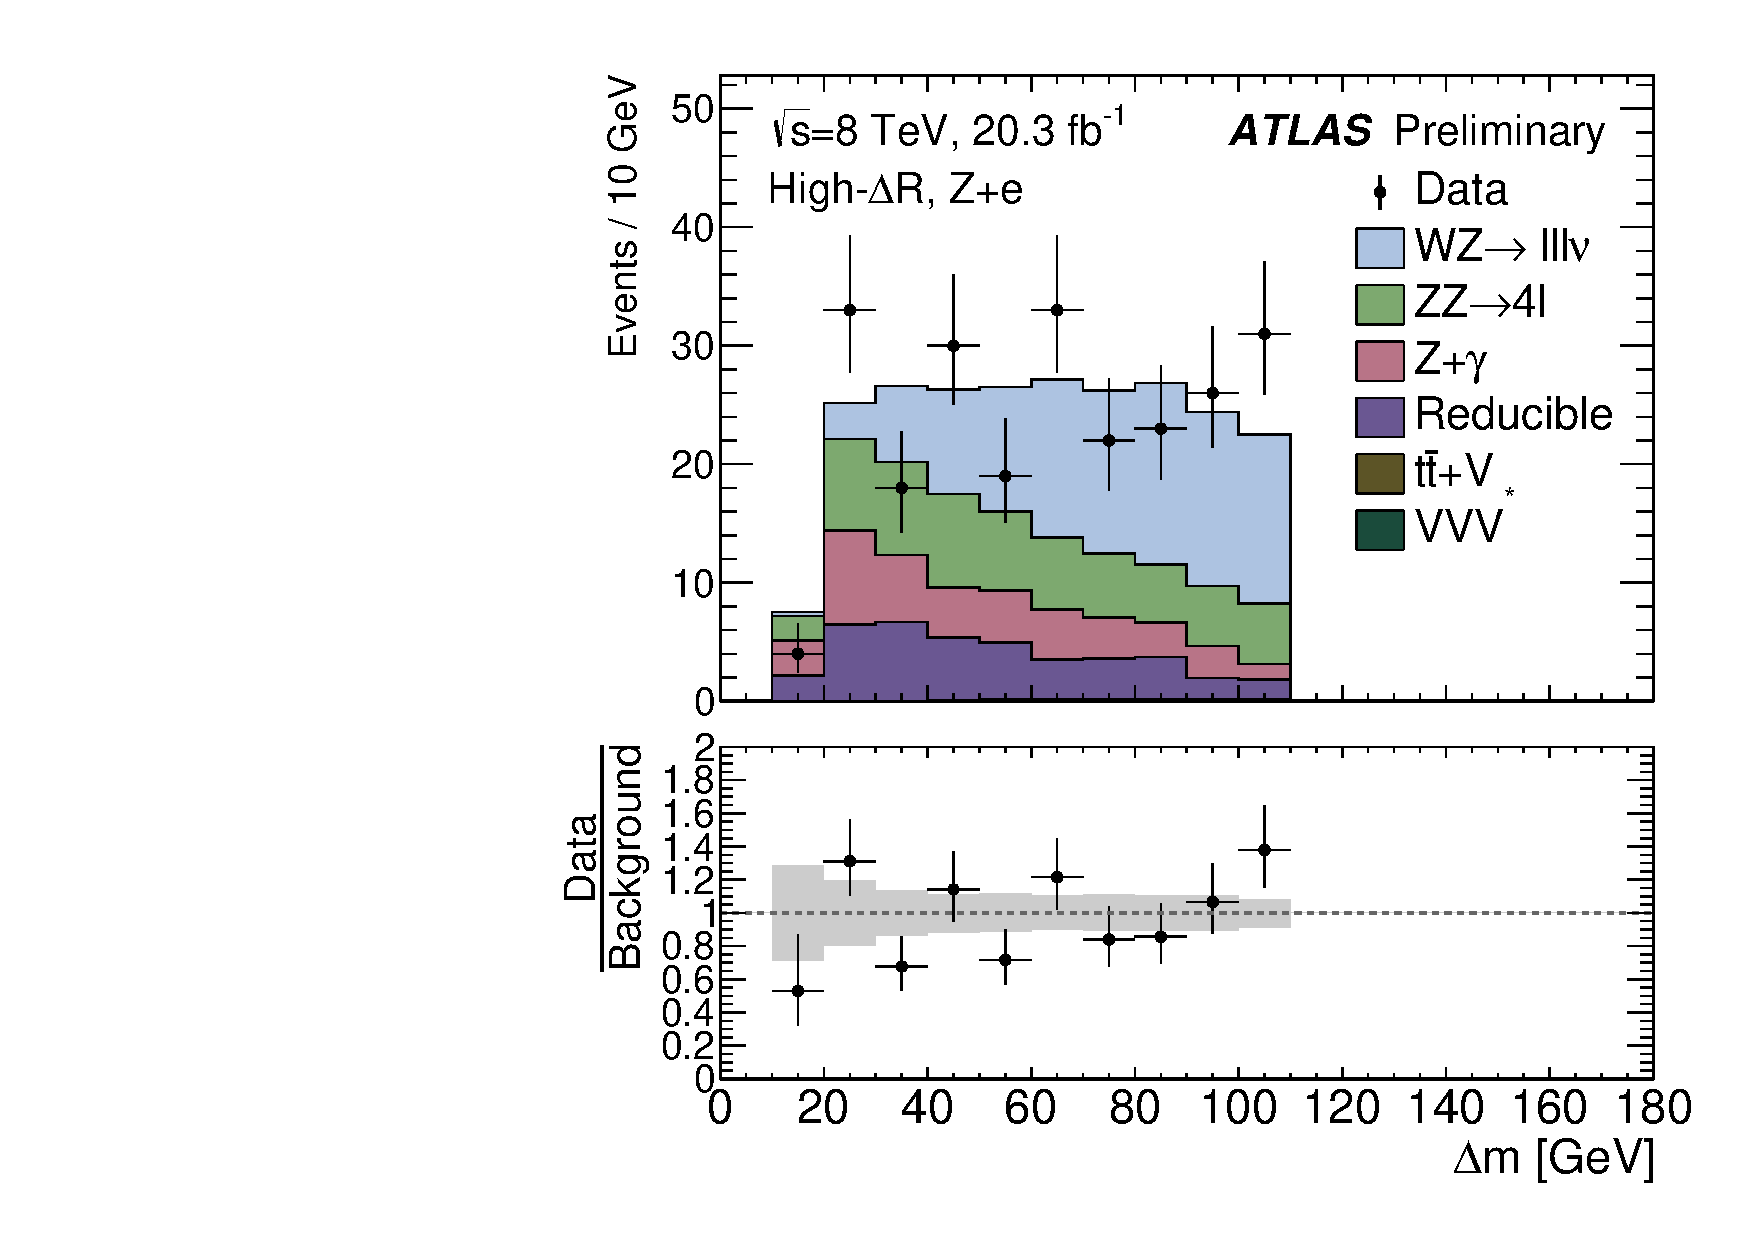
\includegraphics{figures/resonance/c_output_DeltaM_Ze_HighDeltaR_300GeV}}
	}
	\subfloat[ $Z+\mu$] {
		\resizebox{3in}{!}{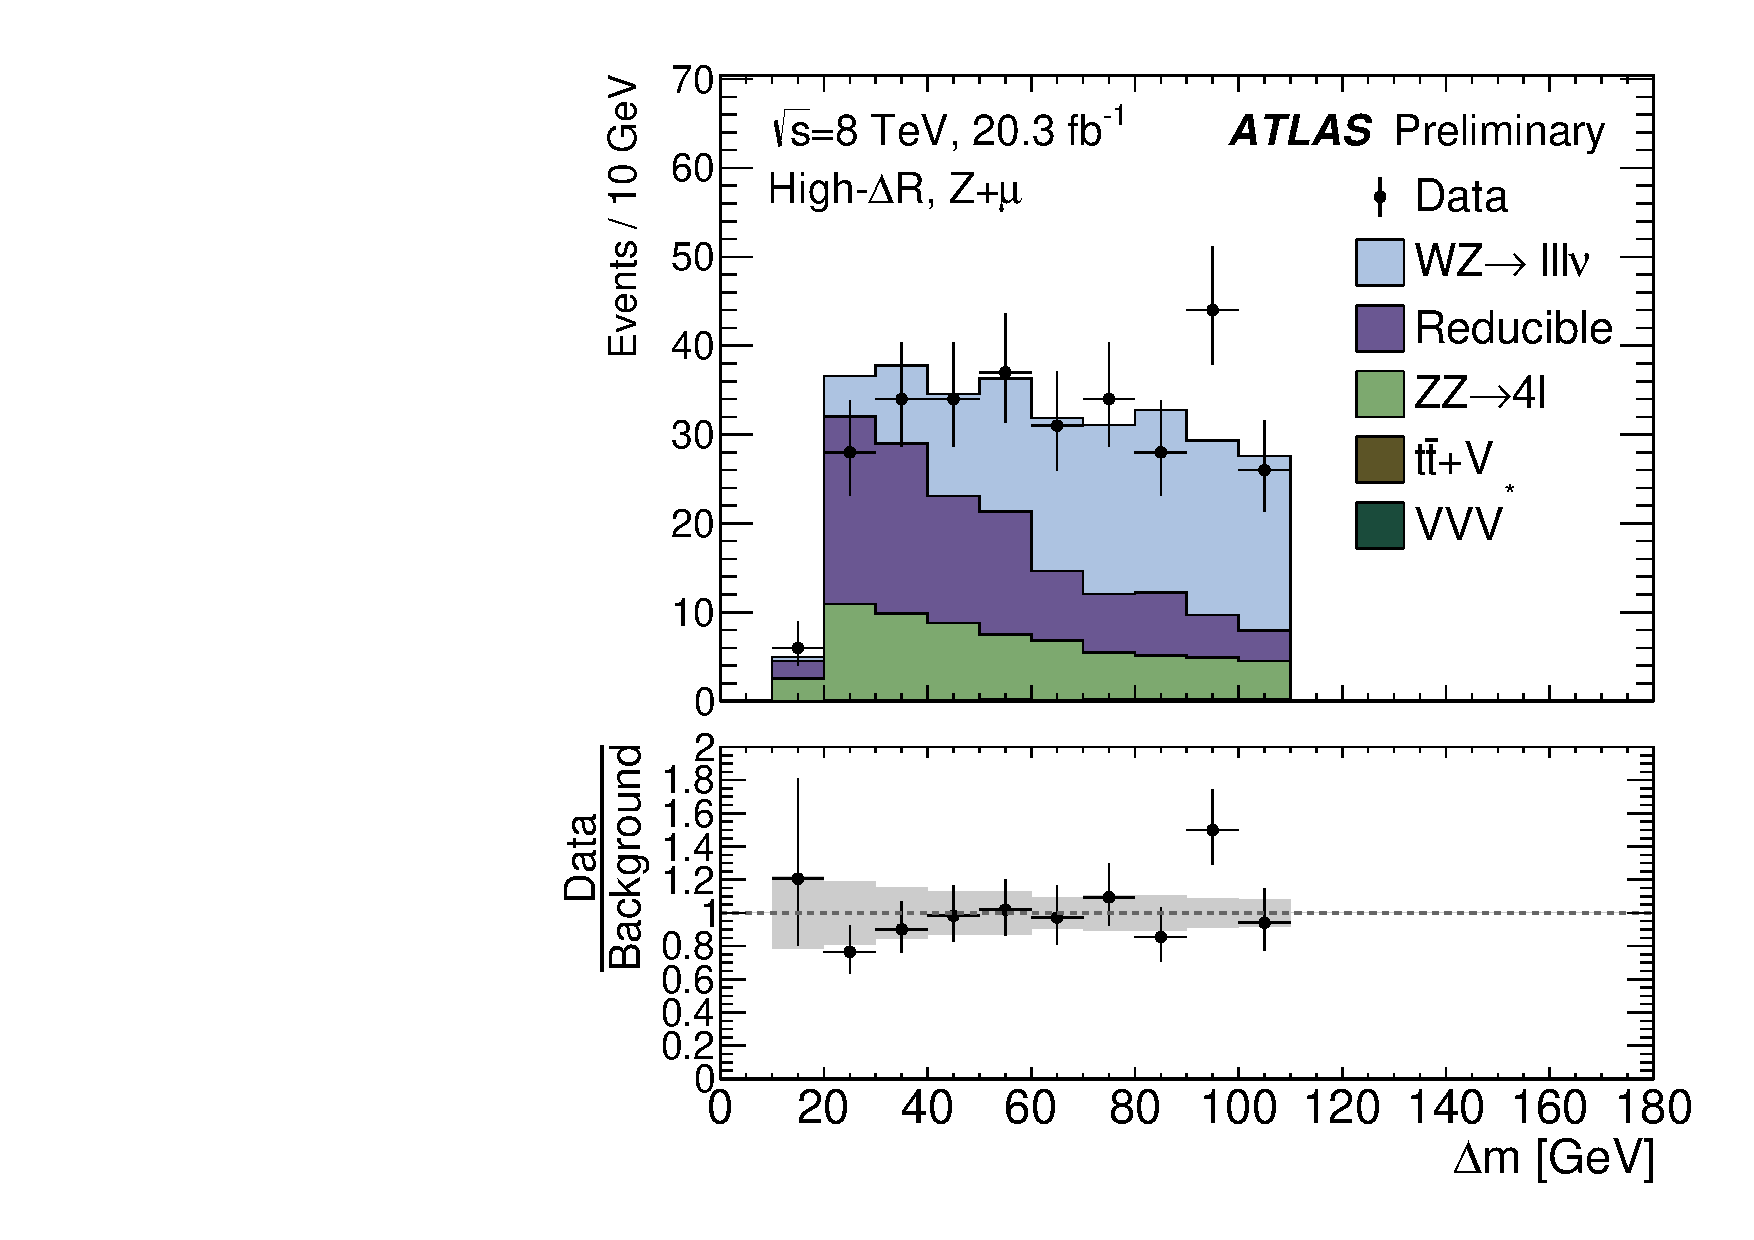
\includegraphics{figures/resonance/c_output_DeltaM_Zmu_HighDeltaR_300GeV}}
	}\\
	\caption{$\deltam$ distributions for the high $\Delta R$ validation regions.}
	\label{fig:resonance-VR-HighDeltaR}
\end{figure}

\begin{figure}[h]
	\centering
	\subfloat[ $Z+e$] {
		\resizebox{3in}{!}{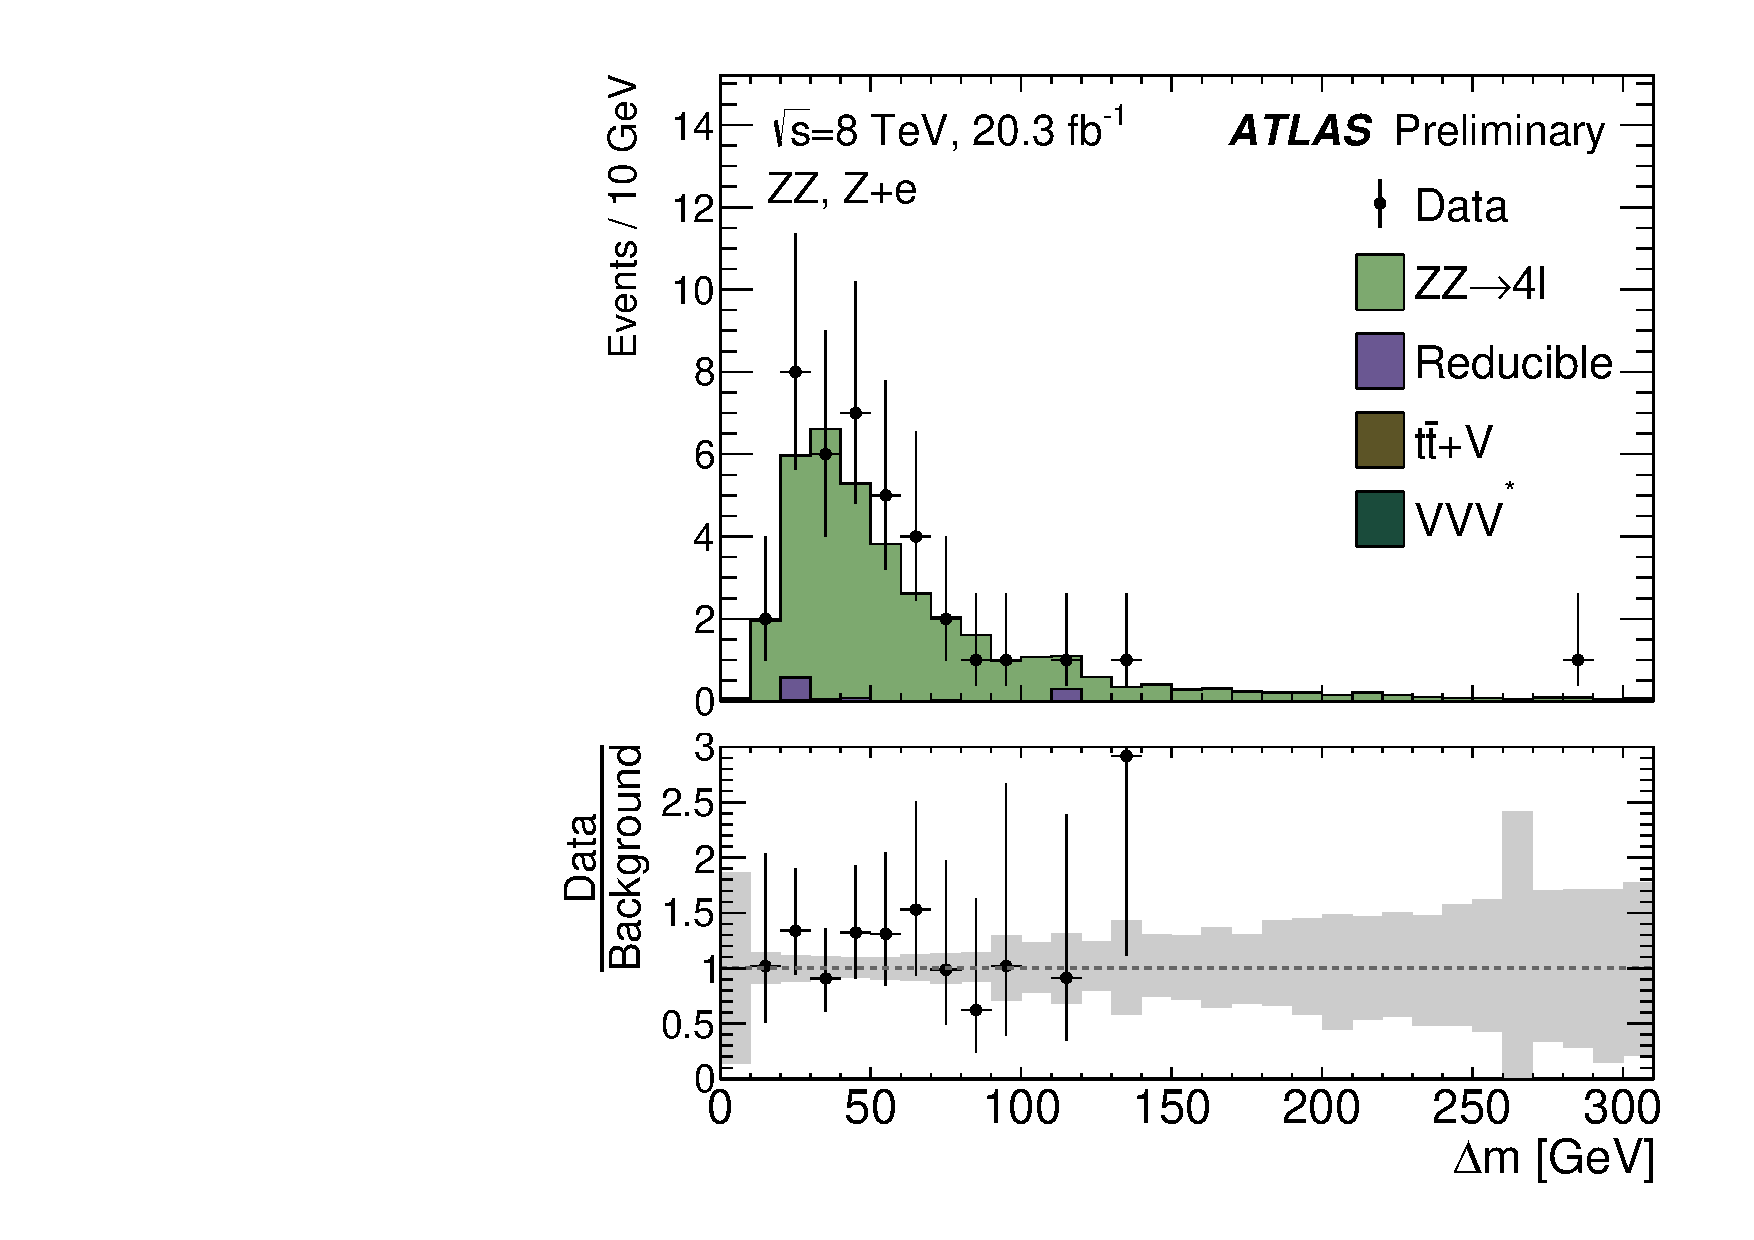
\includegraphics{figures/resonance/c_output_DeltaM_Ze_TwoZ_300GeV}}
	}
	\subfloat[ $Z+\mu$] {
		\resizebox{3in}{!}{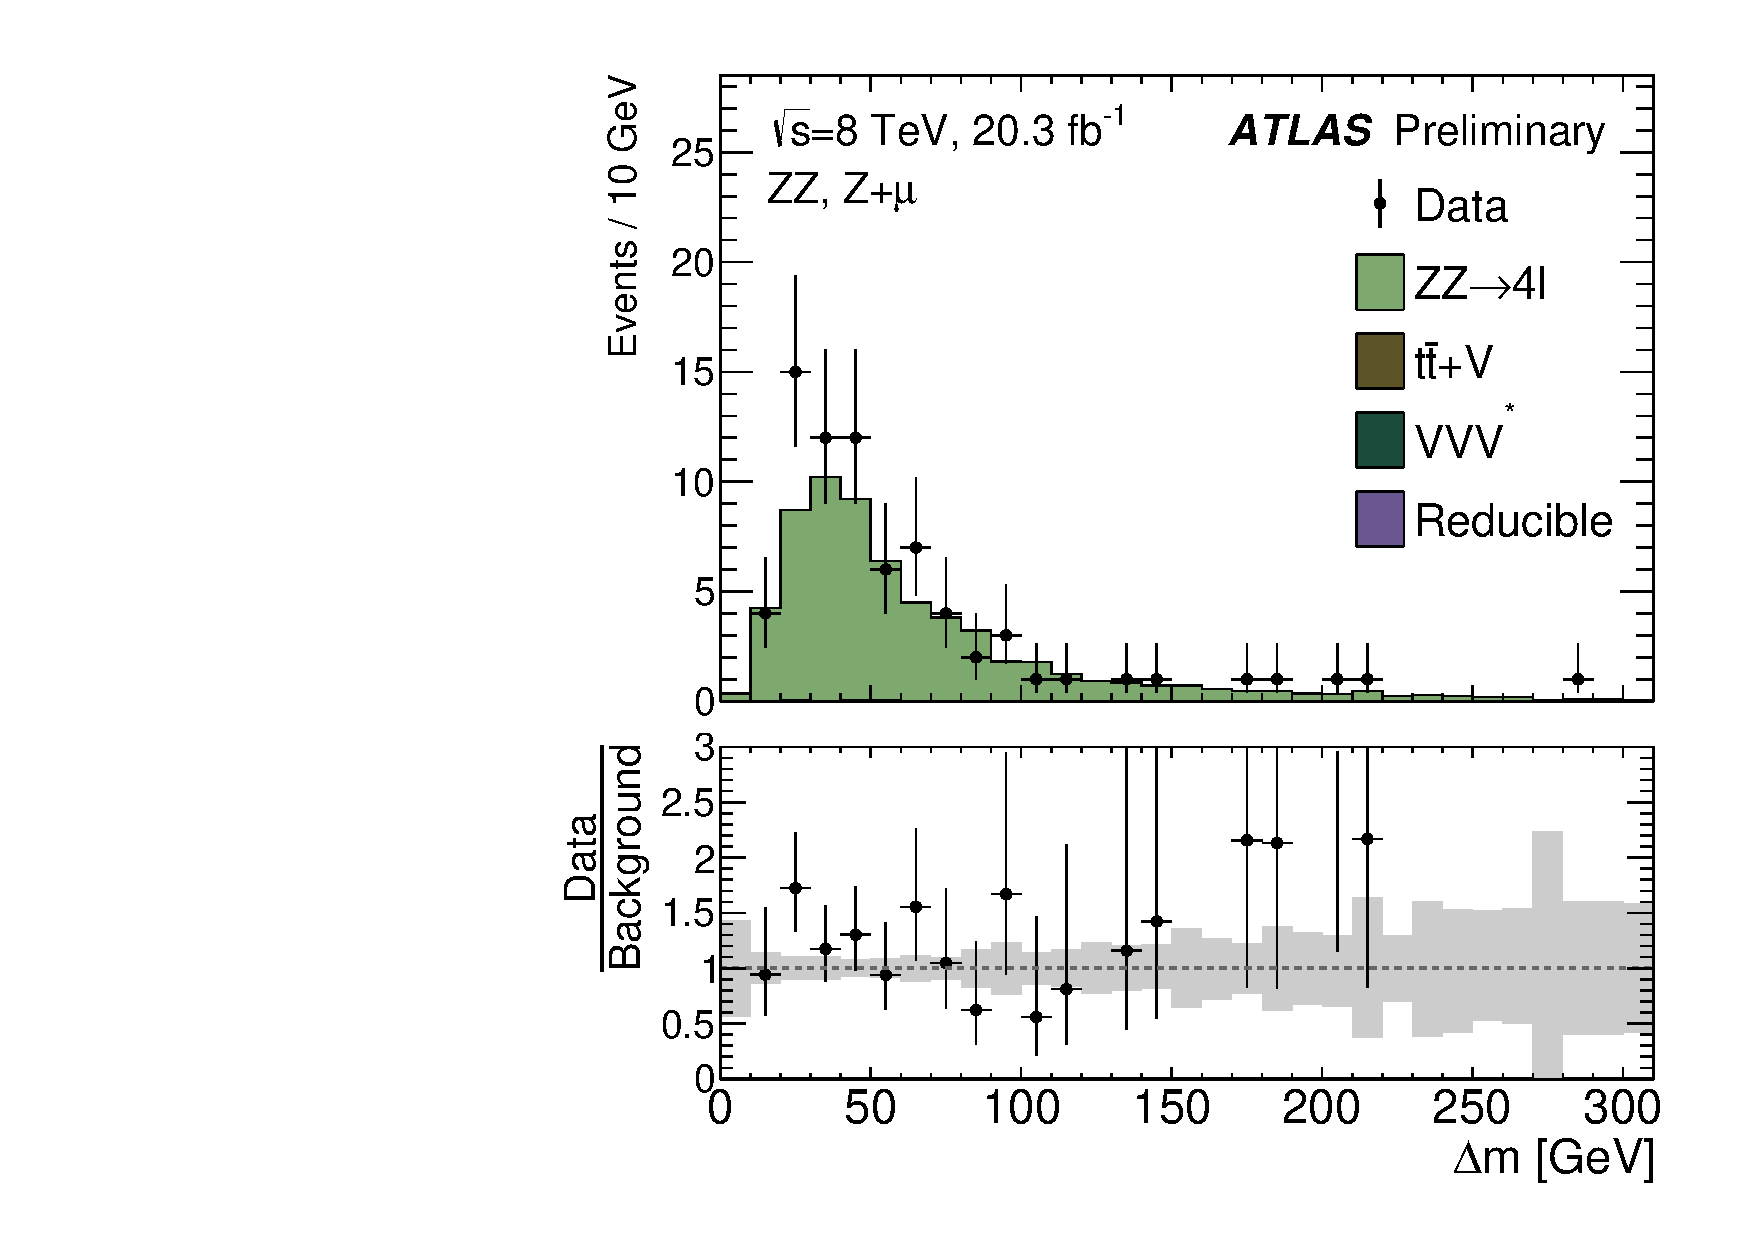
\includegraphics{figures/resonance/c_output_DeltaM_Zmu_TwoZ_300GeV}}
	}\\
	\caption{$\deltam$ distributions for the $ZZ$ validation regions.}
	\label{fig:resonance-VR-ZZ}
\end{figure}

\begin{figure}[h]
	\centering
	\subfloat[ $Z+e$] {
		\resizebox{3in}{!}{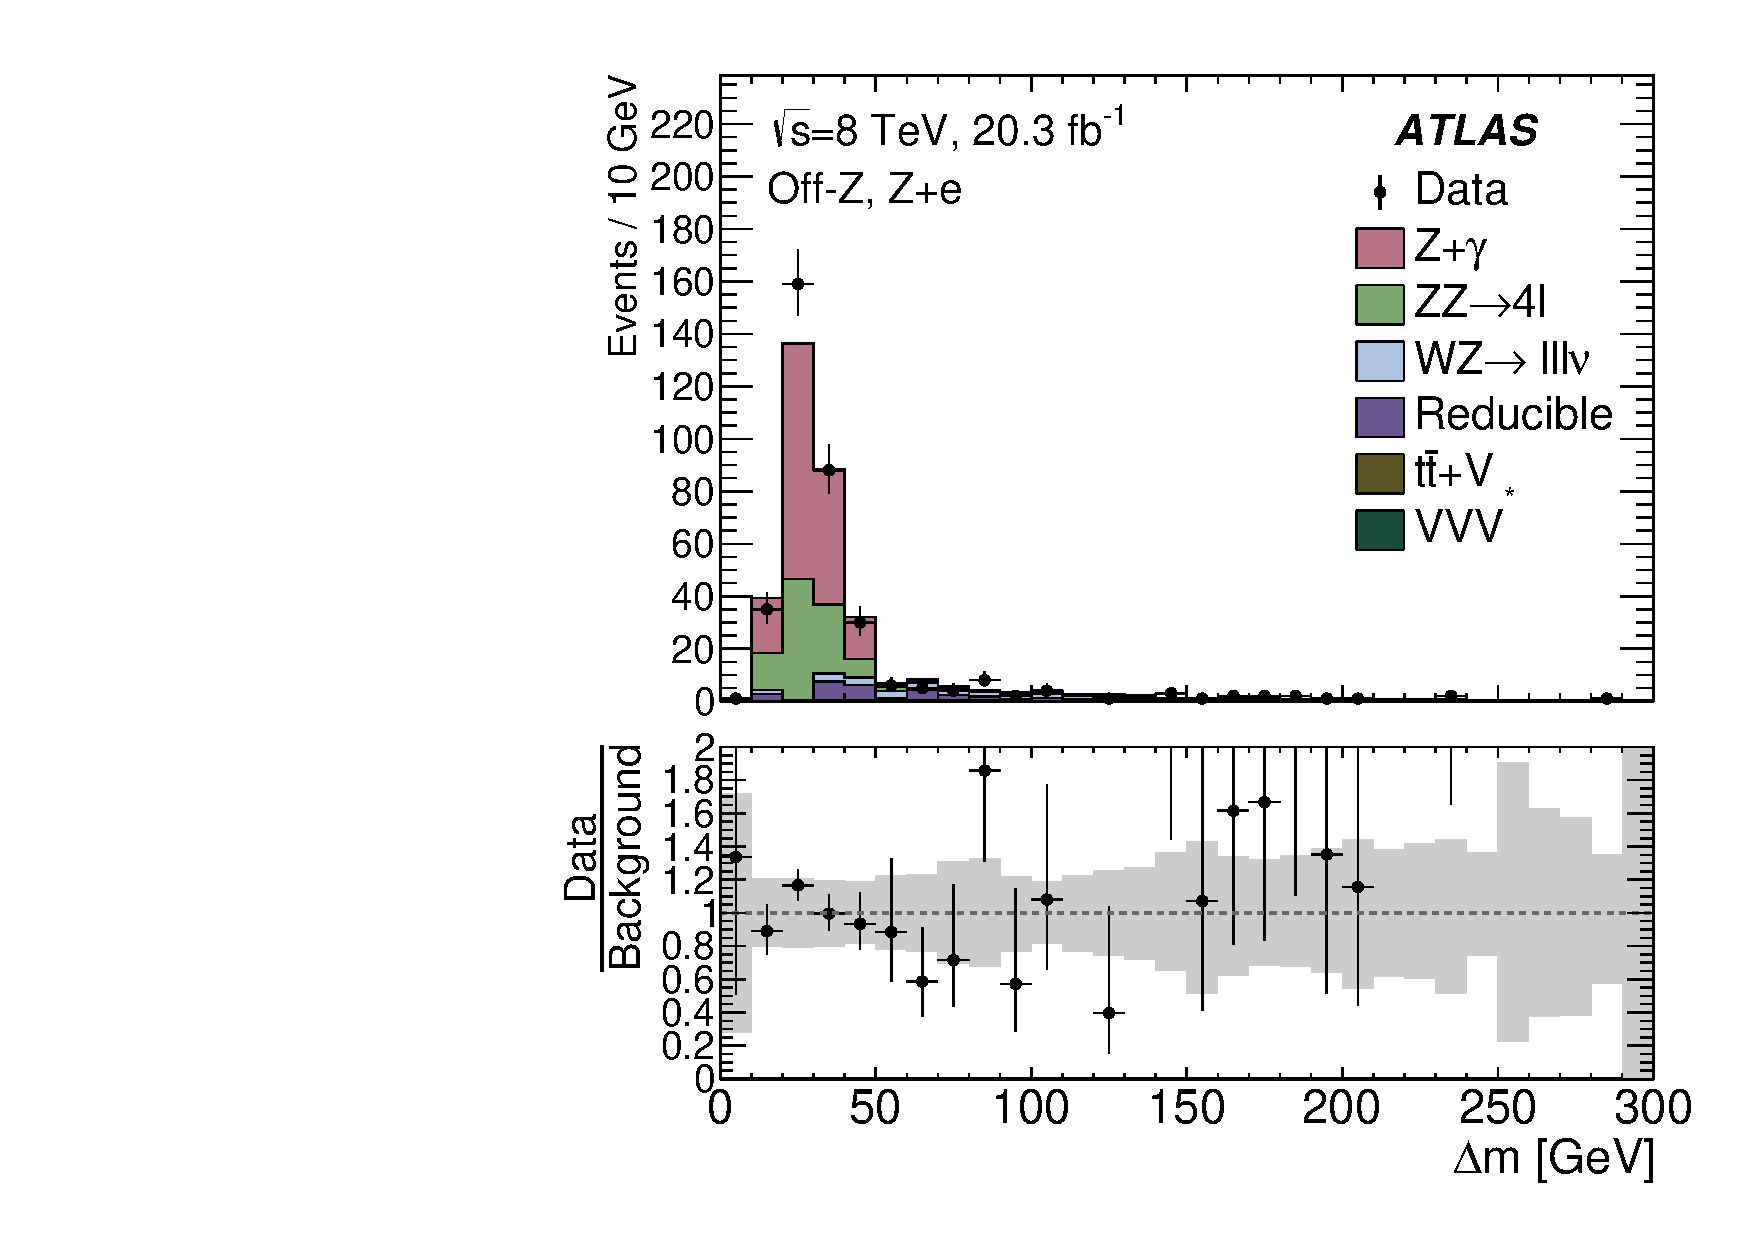
\includegraphics{figures/resonance/c_output_DeltaM_Ze_OffZ_300GeV}}
	}
	\subfloat[ $Z+\mu$] {
		\resizebox{3in}{!}{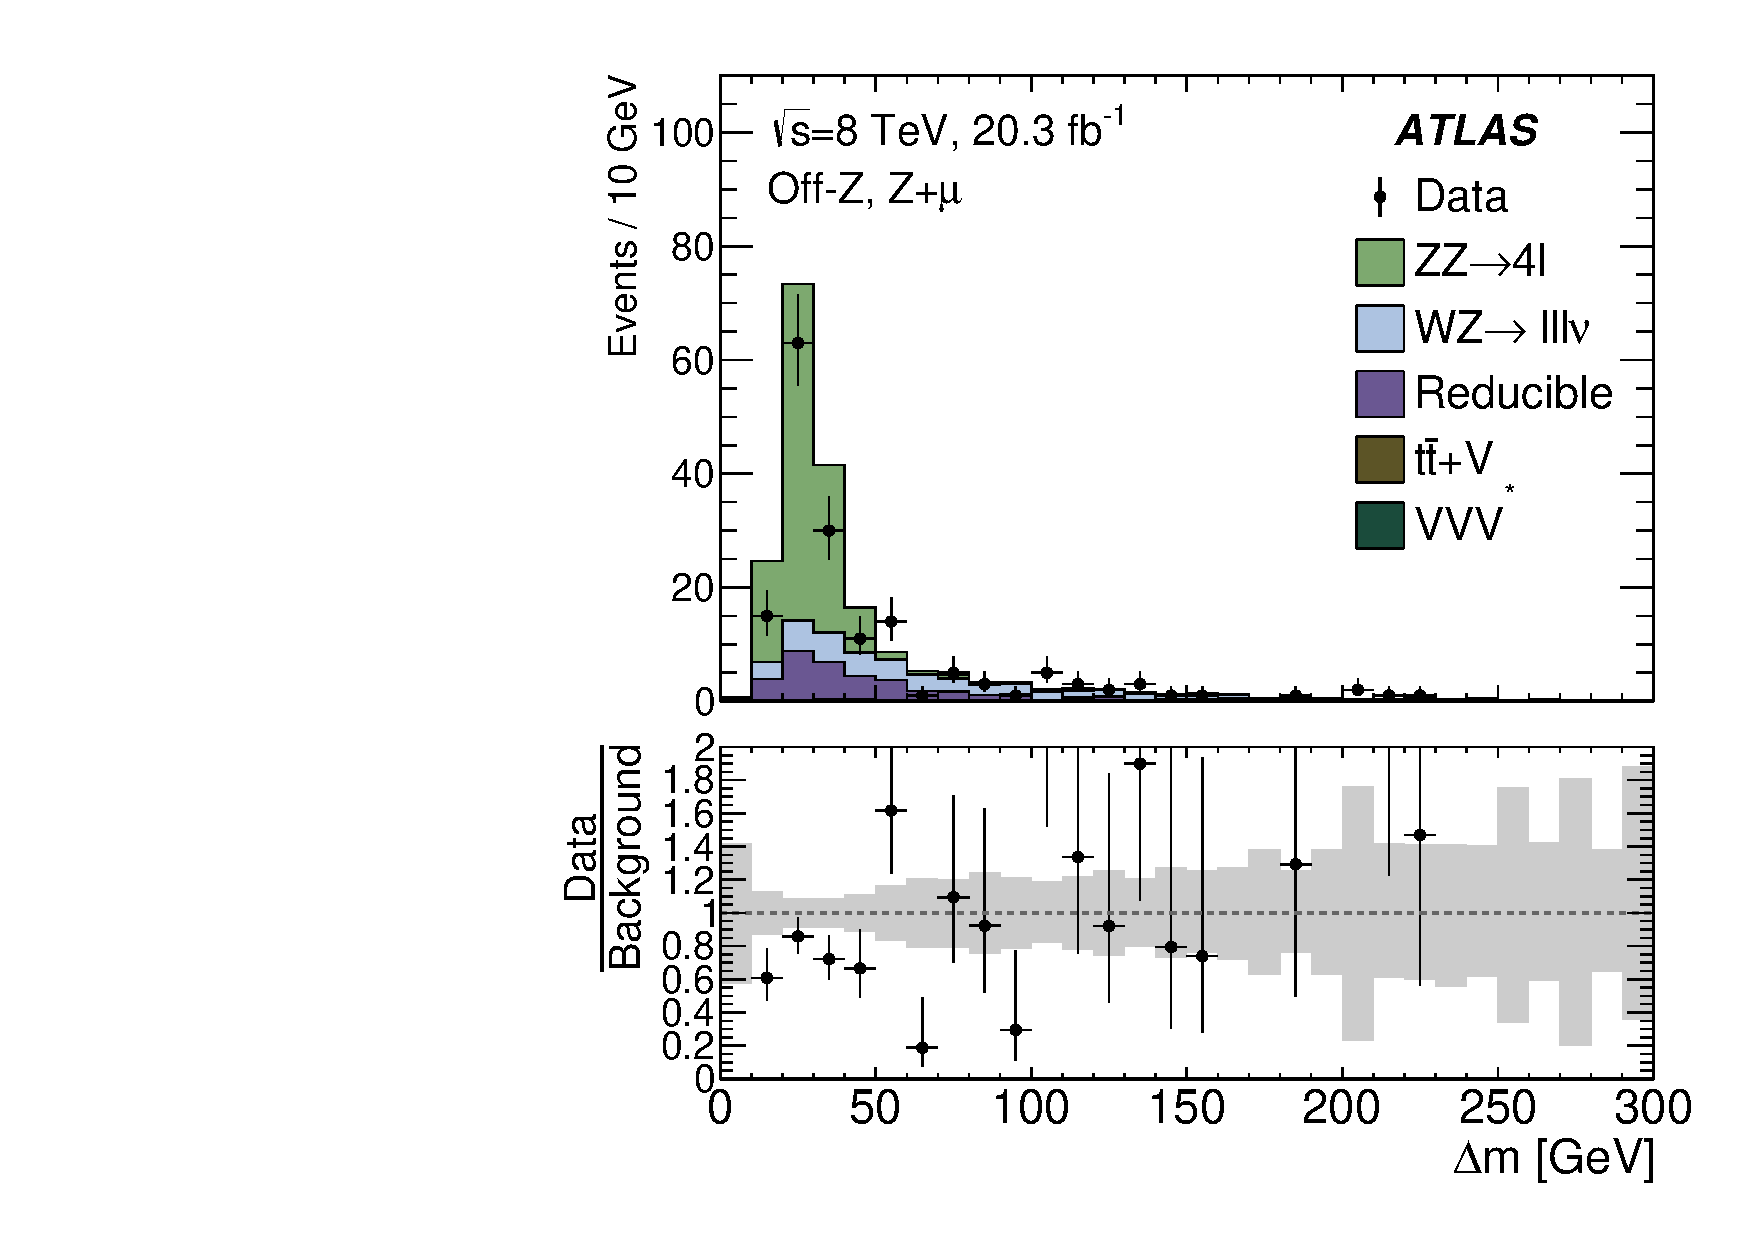
\includegraphics{figures/resonance/c_output_DeltaM_Zmu_OffZ_300GeV}}
	}\\
	\caption{$\deltam$ distributions for the off-$Z$ validation regions.}
	\label{fig:resonance-VR-OffZ}
\end{figure}

\begin{figure}[h]
	\centering
	\subfloat[ $Z+e$] {
		\resizebox{3in}{!}{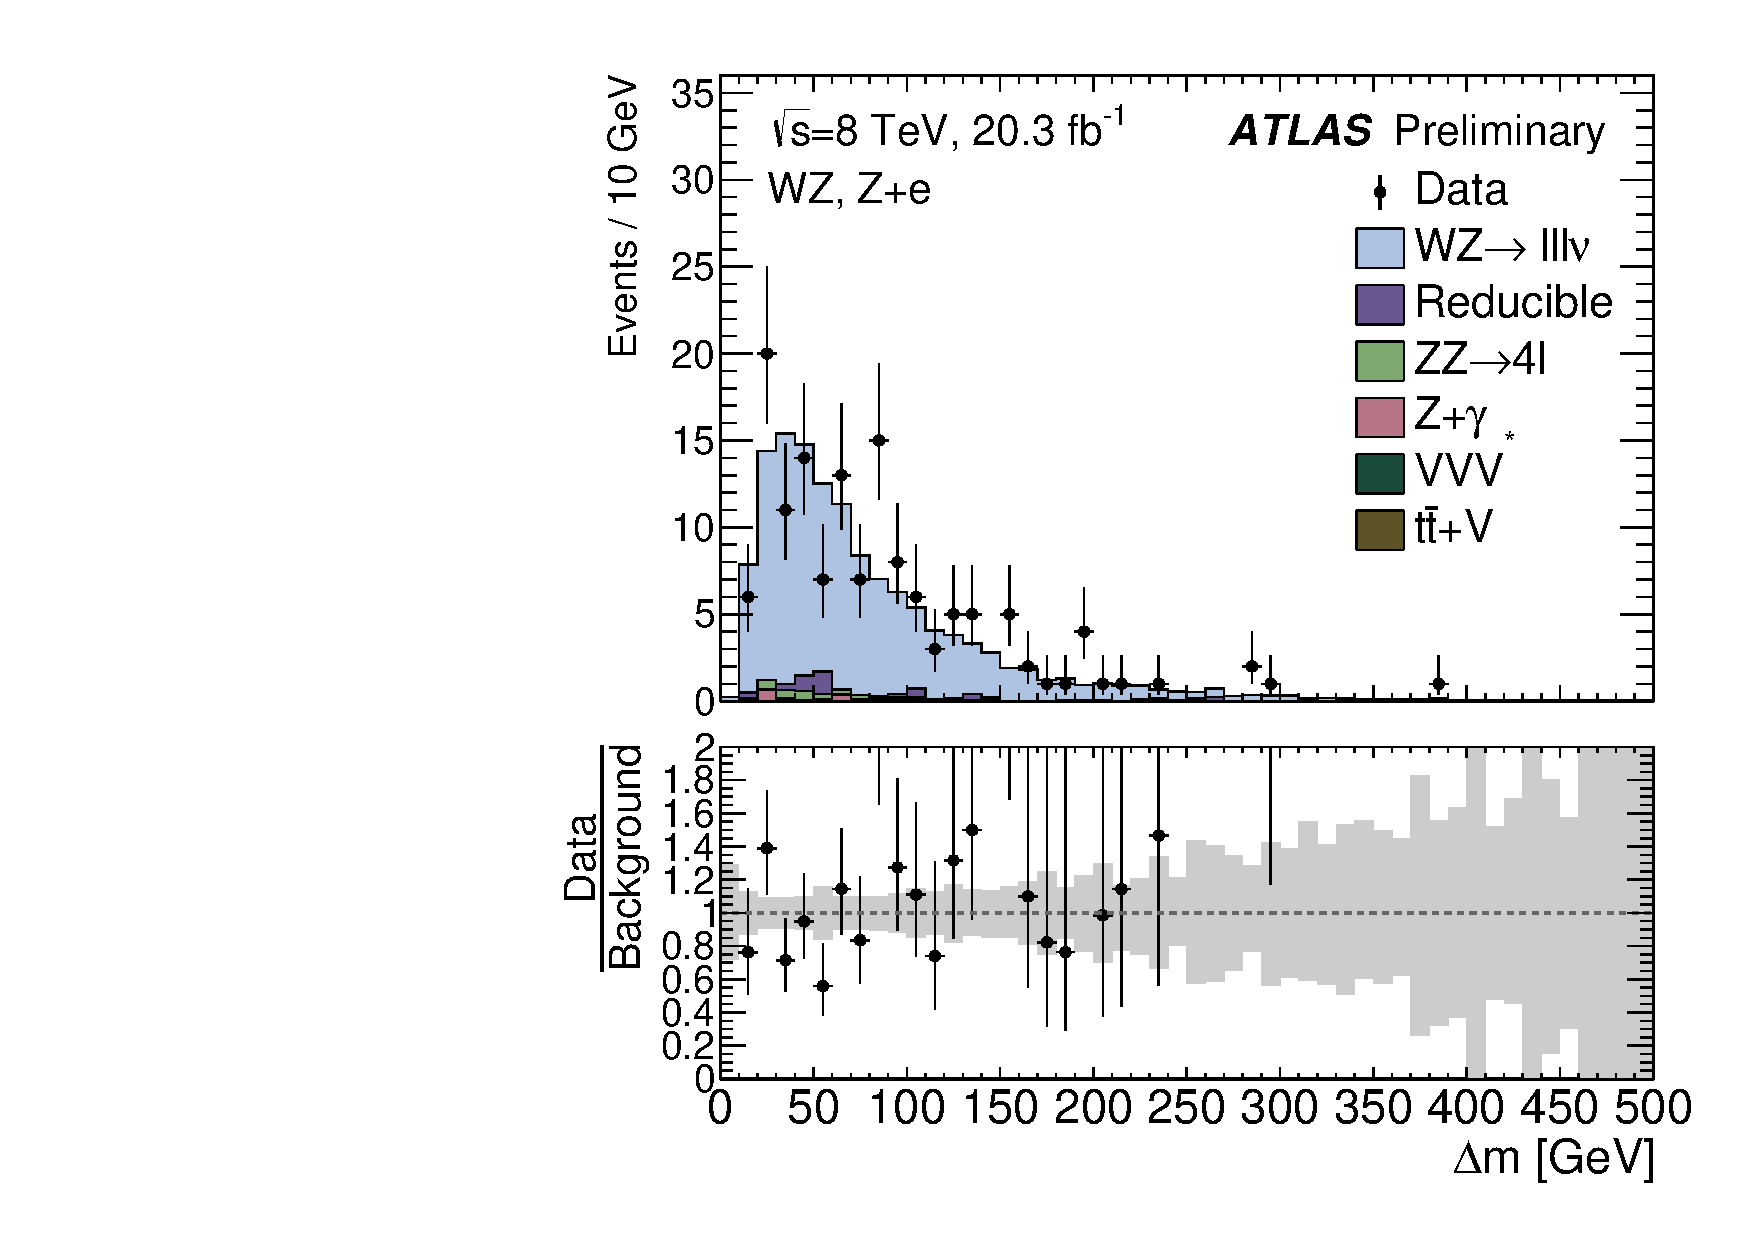
\includegraphics{figures/resonance/c_output_DeltaM_Ze_WZ_300GeV}}
	}
	\subfloat[ $Z+\mu$] {
		\resizebox{3in}{!}{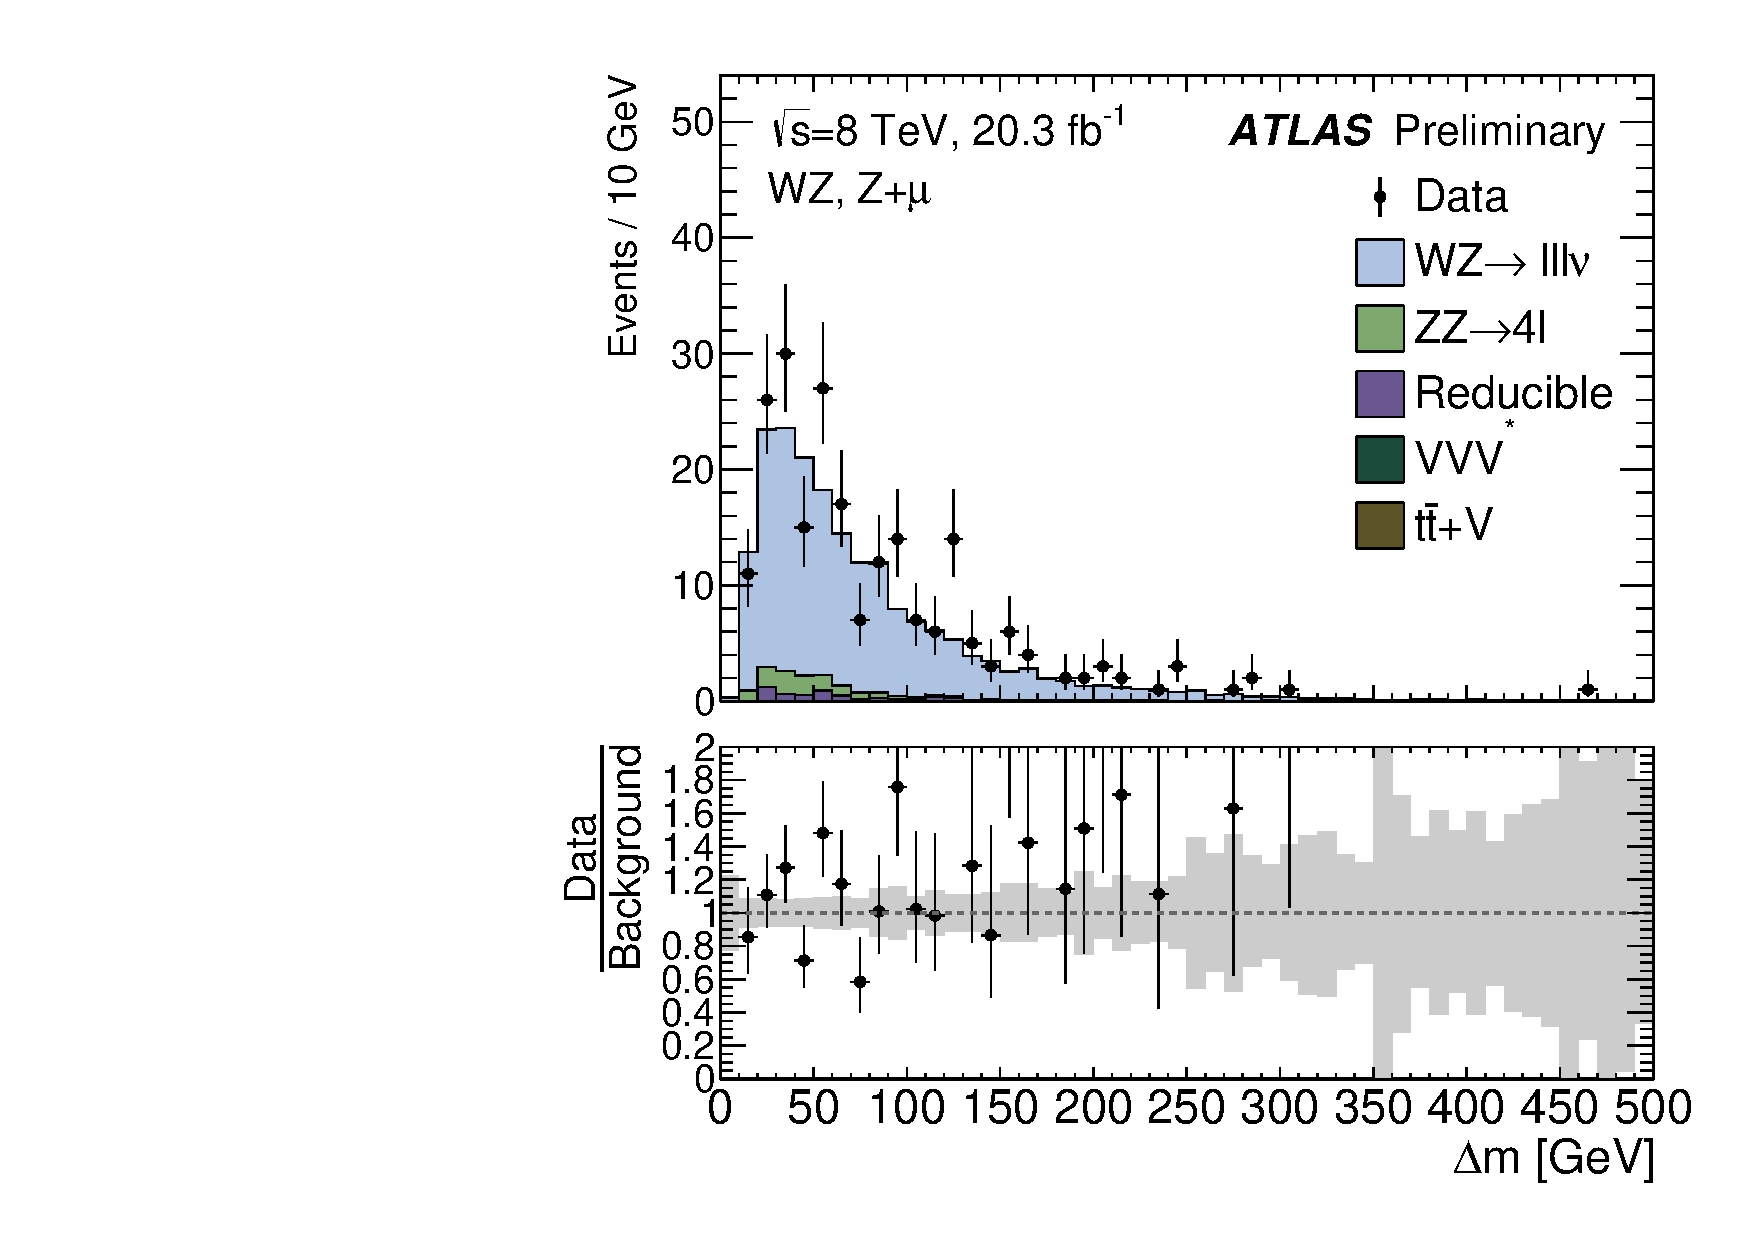
\includegraphics{figures/resonance/c_output_DeltaM_Zmu_WZ_300GeV}}
	}\\
	\caption{$\deltam$ distributions for the $WZ$ validation regions.}
	\label{fig:resonance-VR-WZ}
\end{figure}

\clearpage

\section{Signal and Background Fit Model}\label{sec:resonance-fit-method}
The numbers of signal and background candidate events in data are determined from an unbinned maximum-likelihood fit of a combination of signal and background models to the $\deltam$ distributions in each signal region. The signal and background processes are modelled with analytical probability density functions (p.d.f.s). The parameters of the p.d.f.s are determined from fits to the $\deltam$ distributions predicted by simulation or the fake factor procedure. Then, in each flavor channel, the data is fitted with the combined signal and background model, performed simultaneously on the three categories. In each signal region, the normalization of the dominant background ($ZZ$ or $WZ$) is a free parameter in the fit. The normalizations of all other backgrounds are constrained to fluctuate according to Gaussian probability distributions with mean and width values equal to the estimates and the total uncertainties before fitting.The uncertainties on the p.d.f. parameters are incorporated as Gaussian-distributed nuisance parameters.

\subsection{Signal Modeling}\label{sec:resonance-signal-model}
The $\deltam$ distributions for the type~III seesaw and vector-like leptons scenarios contain two distinct pieces: a peak associated with the correct identification of the three leptons due to the heavy lepton decay, and a broader component due to cases where the trilepton candidate does not originate from a heavy lepton decay. Accordingly, the distributions are modeled using the sum of two functions: a Voigtian for the peak and a Landau function for the combinatorial component.  The signal parametrization is given by the following expression: 

\begin{align}\label{eqn:resonance-signal-parametrization}
\mathcal{S}(m_\lpm) &= f_V F_V(\deltam; \Gamma_V, m_V,  \sigma_V ) + (1-f_V)F_L(\deltam; \sigma_L, m_L), \\
%F_V(x; \Gamma_V, m_V, \sigma_V) &= \int_{-\infty}^{\infty} G(x'; \sigma_V) L(x-m_V-x'; \Gamma_V),\ \mbox{where } G(x;\sigma_V)=\frac{e^{-x^2/(2\sigma_V^2)}}{\sigma\sqrt{2\pi}}\ \mbox{and } L(x;\Gamma_V)=\frac{\Gamma_V}{\pi(x^2+\Gamma_v^2)}, \\
%F_L(x; \\sigma_L,m_L) &= ?
\end{align}
where $f_V$ denotes the fraction of events in the Voigtian; $\Gamma_V$, $m_V$ and $\sigma_V$ are the width, mean and gaussian smearing term of the Voigtian; and $\sigma_L$ and $m_L$ are the width and mean of the Landau distribution.  

\begin{figure}[H!]
\begin{minipage}[c]{\textwidth}
  \centering
 % \includegraphics[width=0.48\textwidth]{figures/Liv/Fit/sig120_Fit.pdf}
 \subfloat[ $m_{3\ell}$ ] {
		\resizebox{0.48\textwidth}{!}{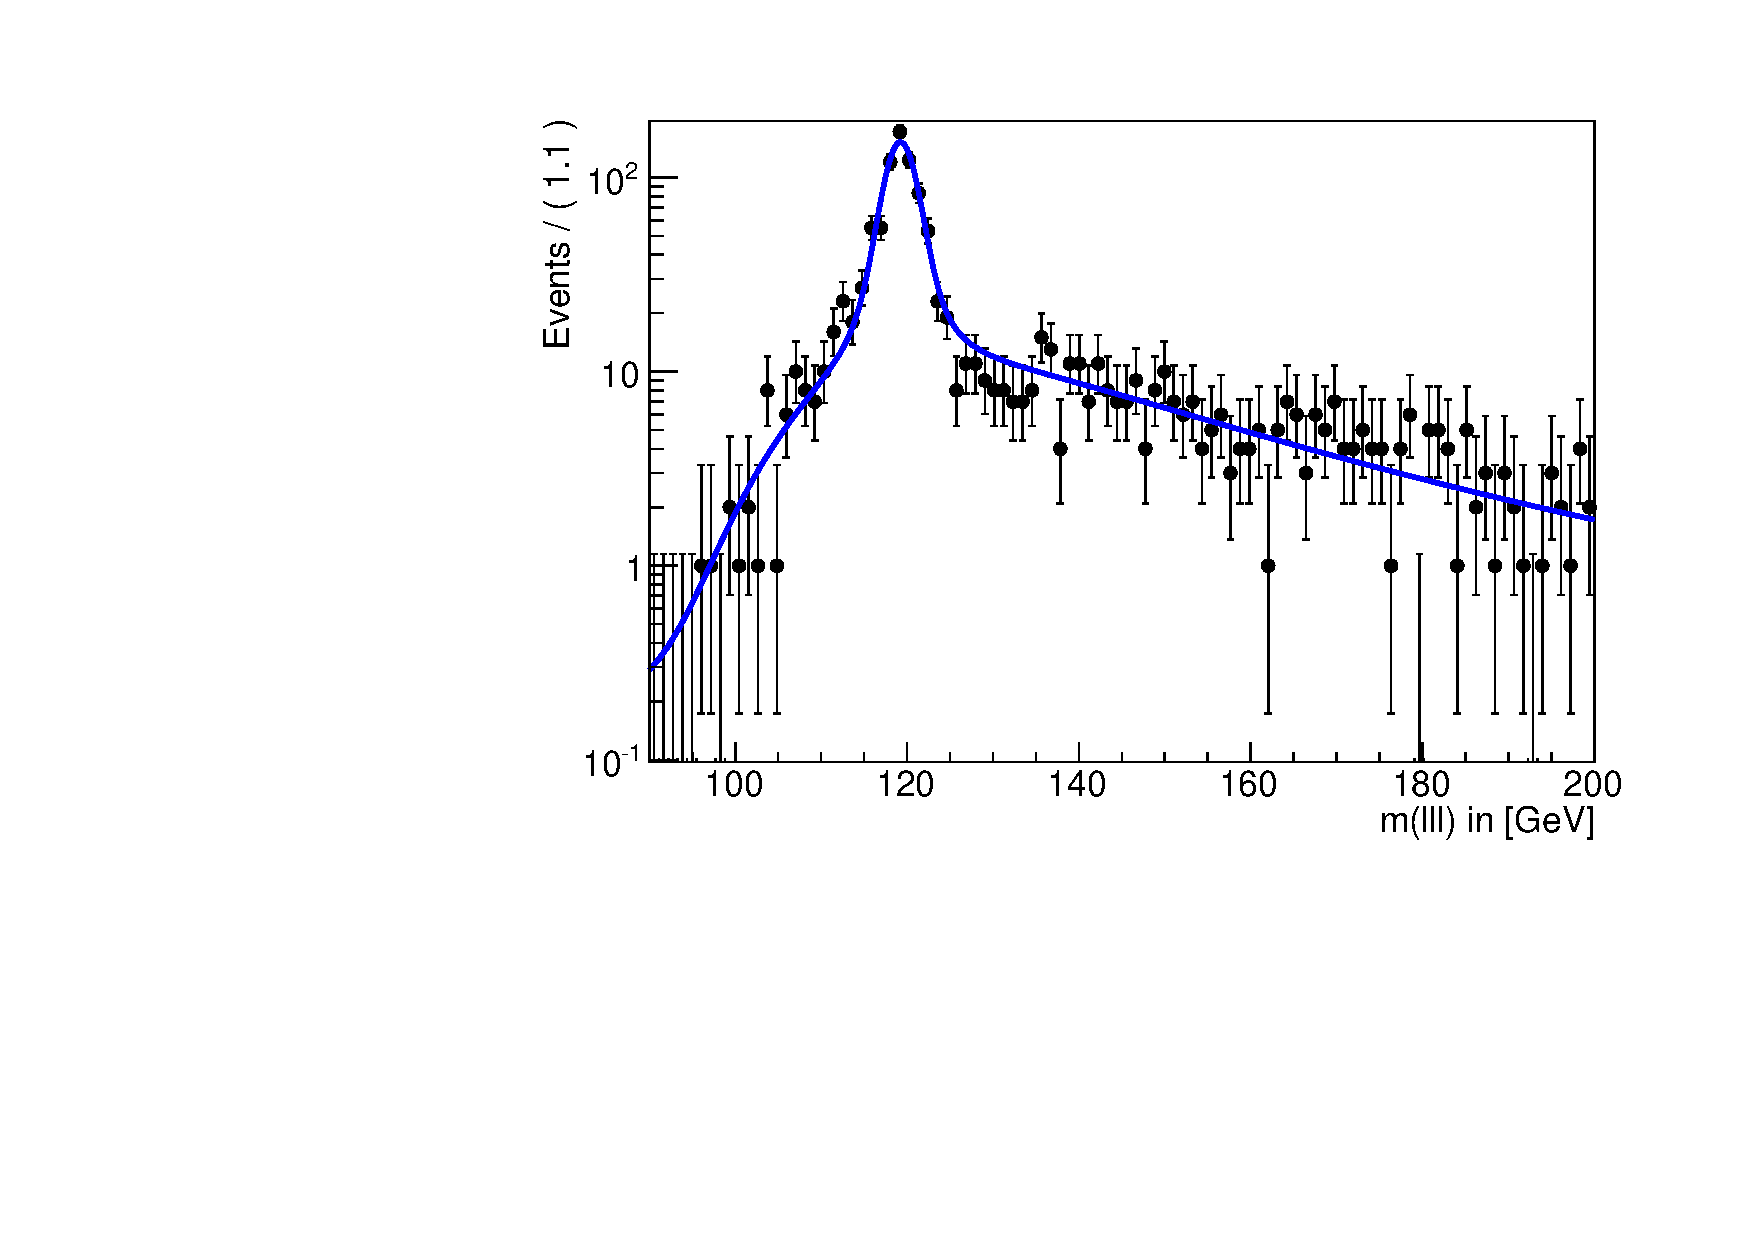
\includegraphics{figures/resonance/Fit_sig120_Fit.pdf}}
	}
	\subfloat[$\deltam$ ] {
		\resizebox{0.48\textwidth}{!}{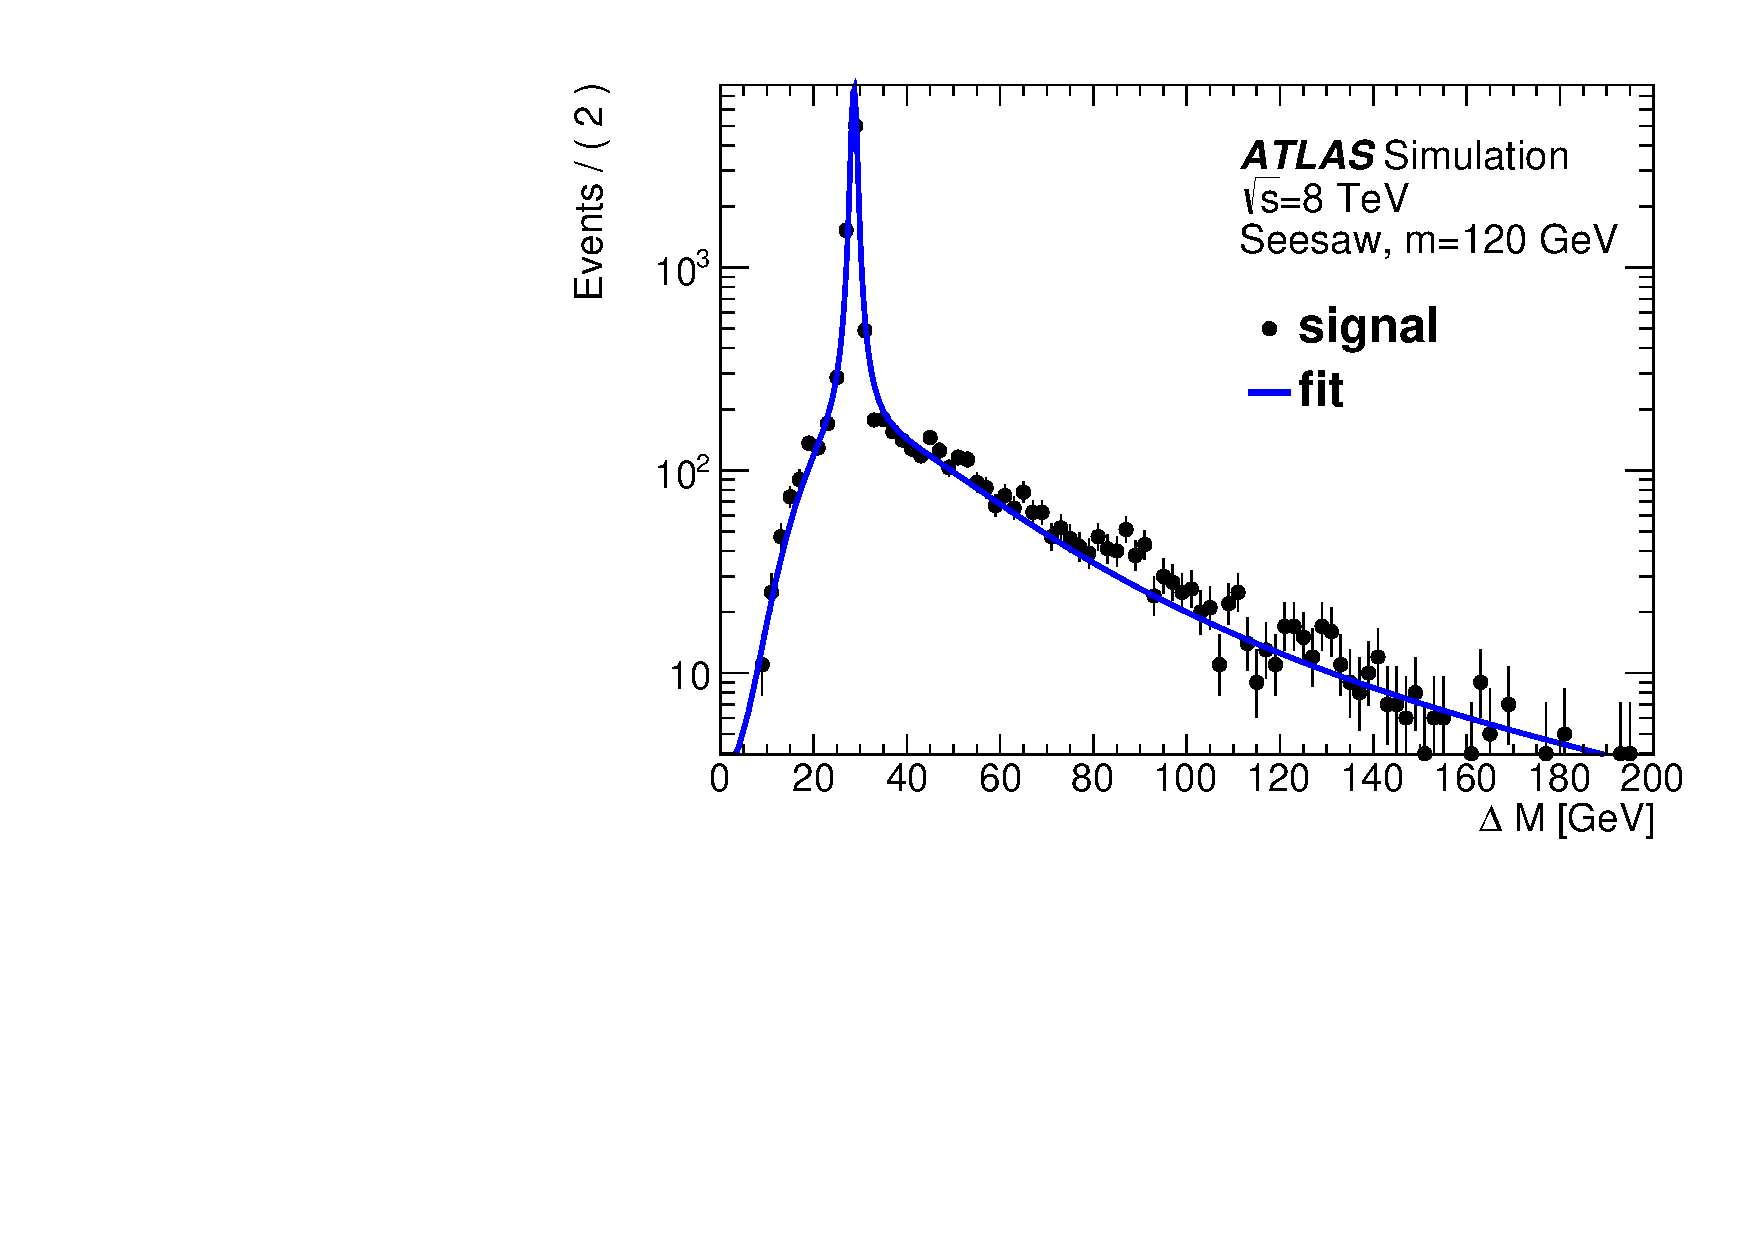
\includegraphics{figures/resonance/Seesaw_inclusive_sig120_Fit.pdf}}
	}
  \caption{$m_{3\ell}$ and $\deltam$ distributions for the 120 GeV signal mass point fitted the sum of a Voigtian and a Landau PDF. The fit is an unbinned maximum likelihood fit; the data is binned only for presentation.}
  \label{fig:SigFit}
 \subfloat[$m_{3\ell}$ ] {
		\resizebox{0.48\textwidth}{!}{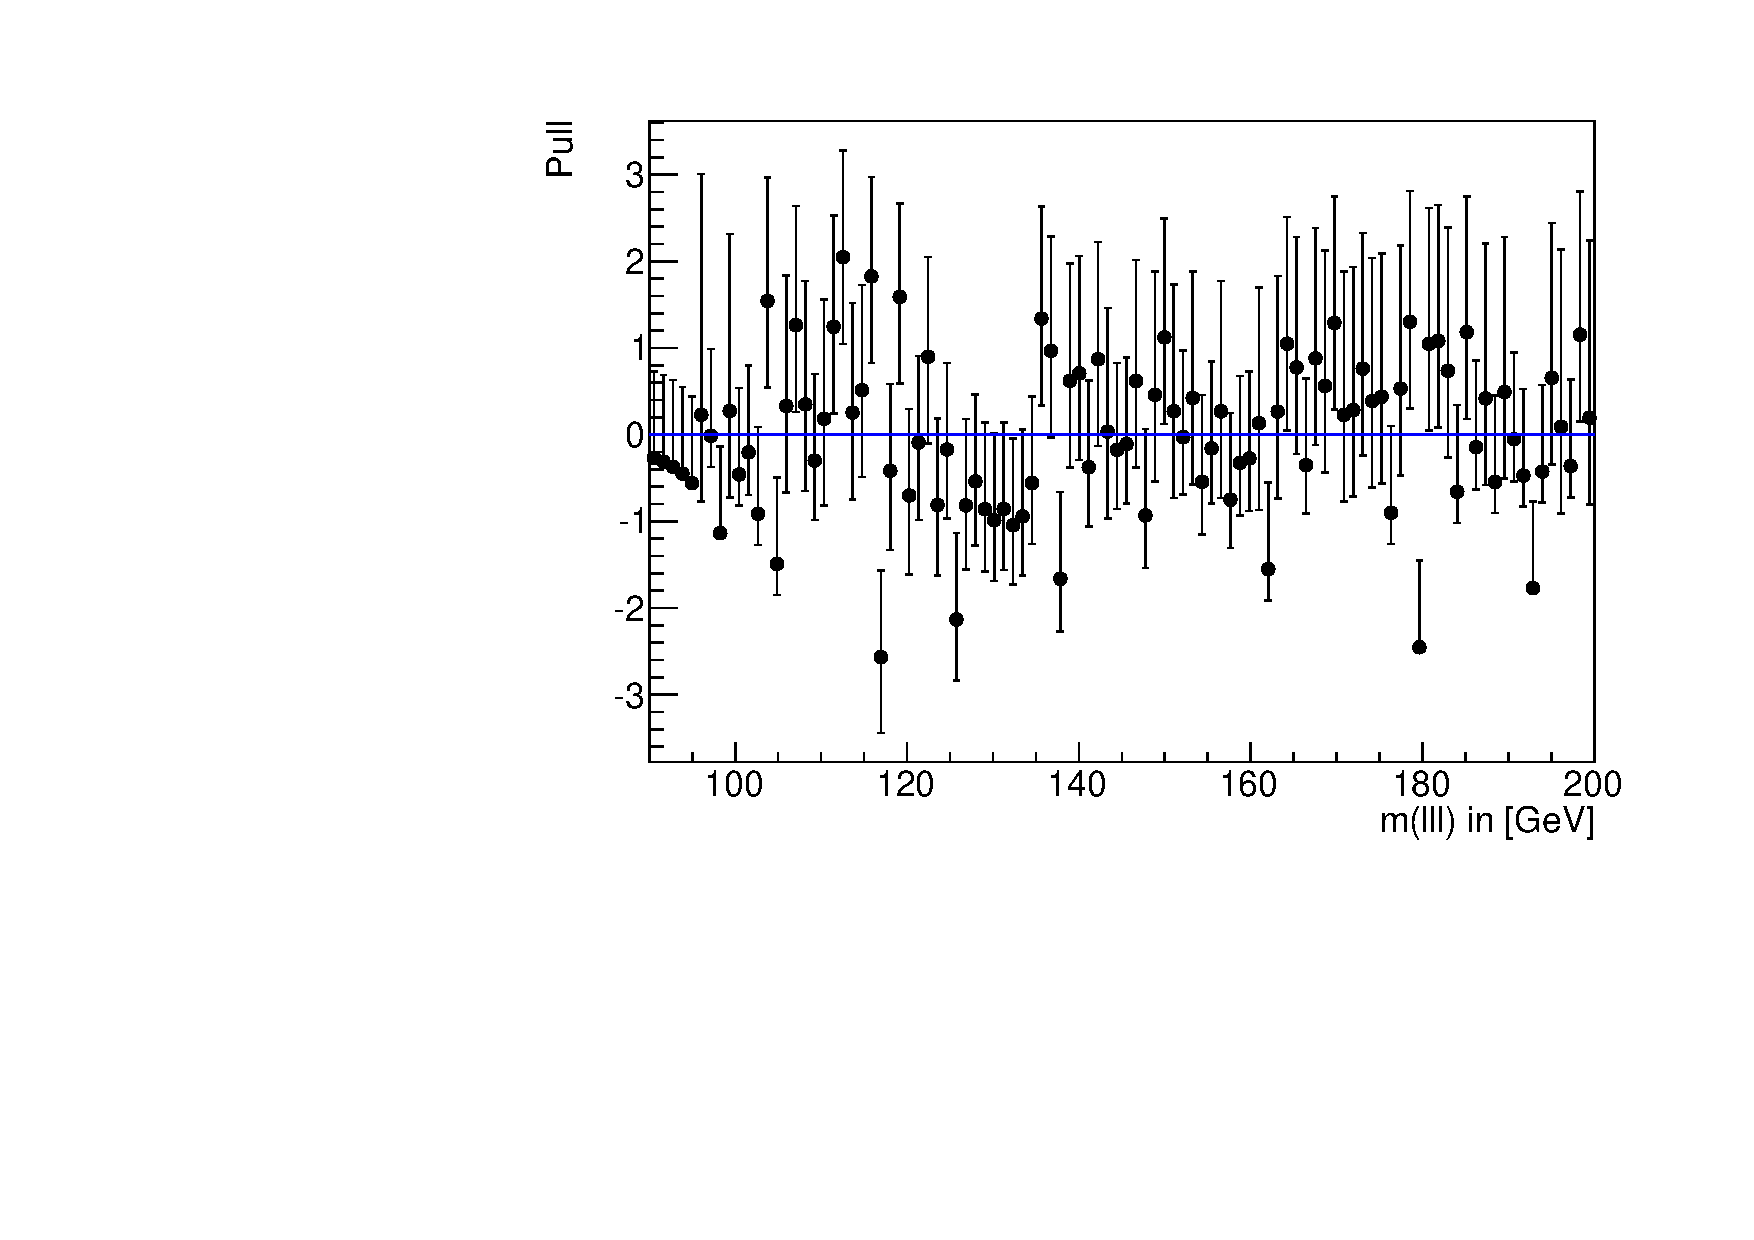
\includegraphics{figures/resonance/Fit_sig120_Pull.pdf}}
	}
	\subfloat[$\deltam$ ] {
		\resizebox{0.48\textwidth}{!}{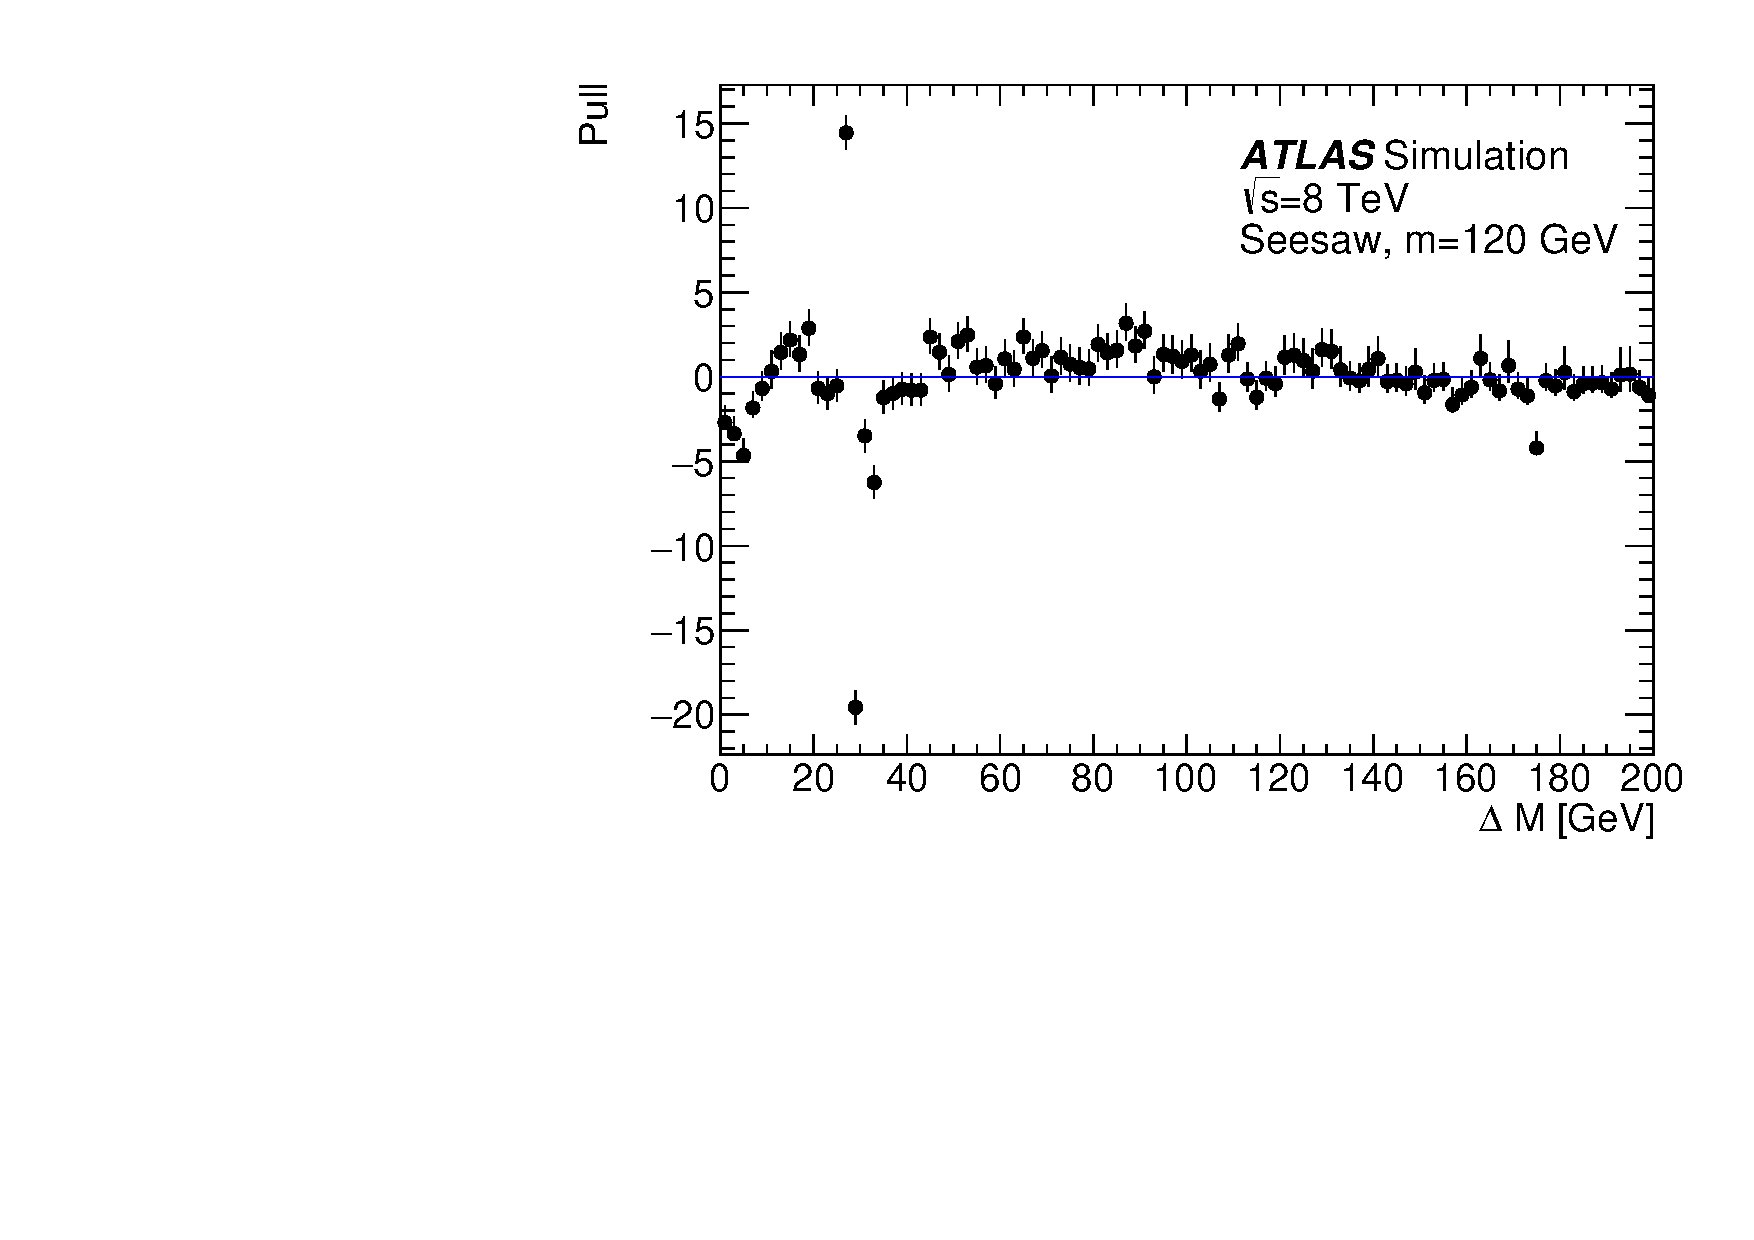
\includegraphics{figures/resonance/Seesaw_inclusive_sig120_Pull.pdf}}
	}
  \caption{Pulls of the simulated data with respect to the fit for $m_{3\ell}$ and $\deltam$ at the 120 GeV signal mass point. }
  \label{fig:Pull}
 \subfloat[$m_{3\ell}$ ] {
		\resizebox{0.48\textwidth}{!}{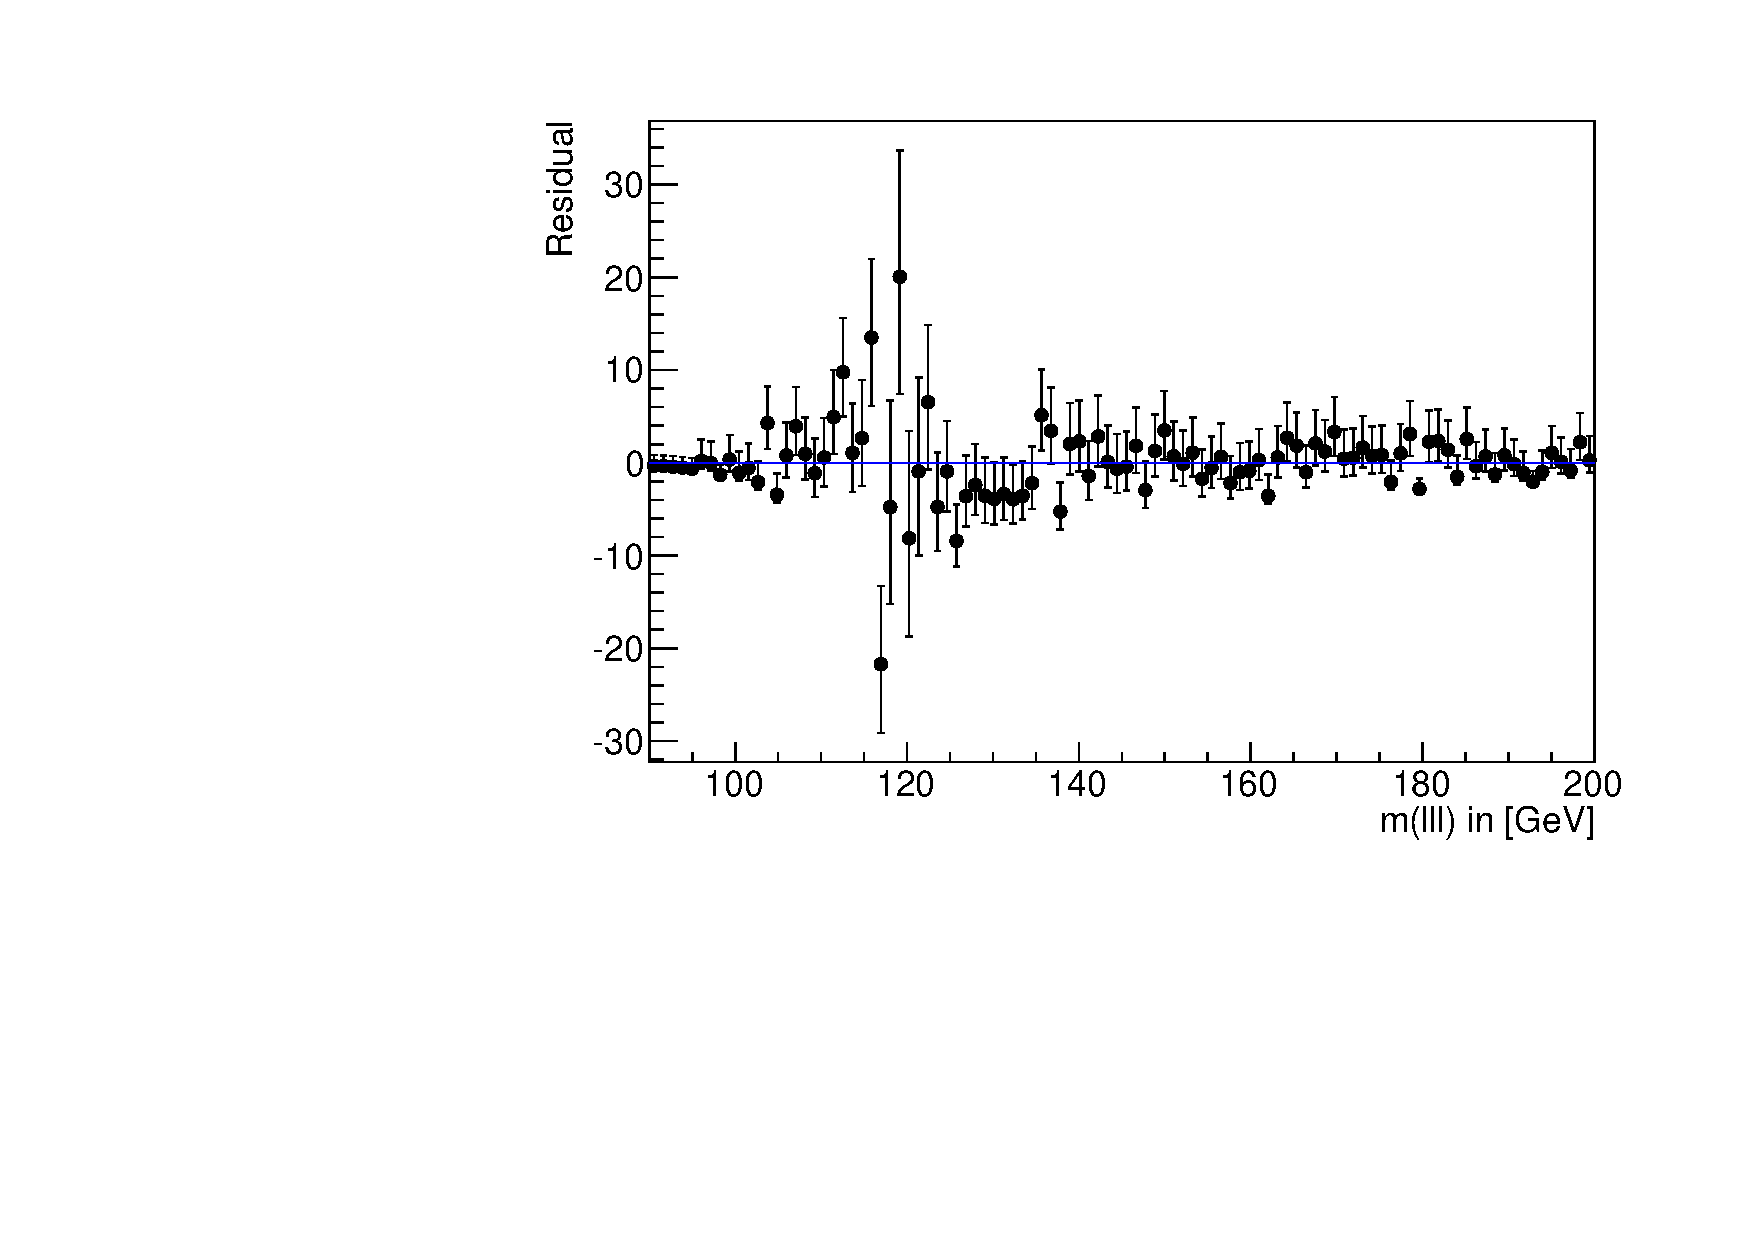
\includegraphics{figures/resonance/Fit_sig120_Resid.pdf}}
	}
	\subfloat[$\deltam$ ] {
		\resizebox{0.48\textwidth}{!}{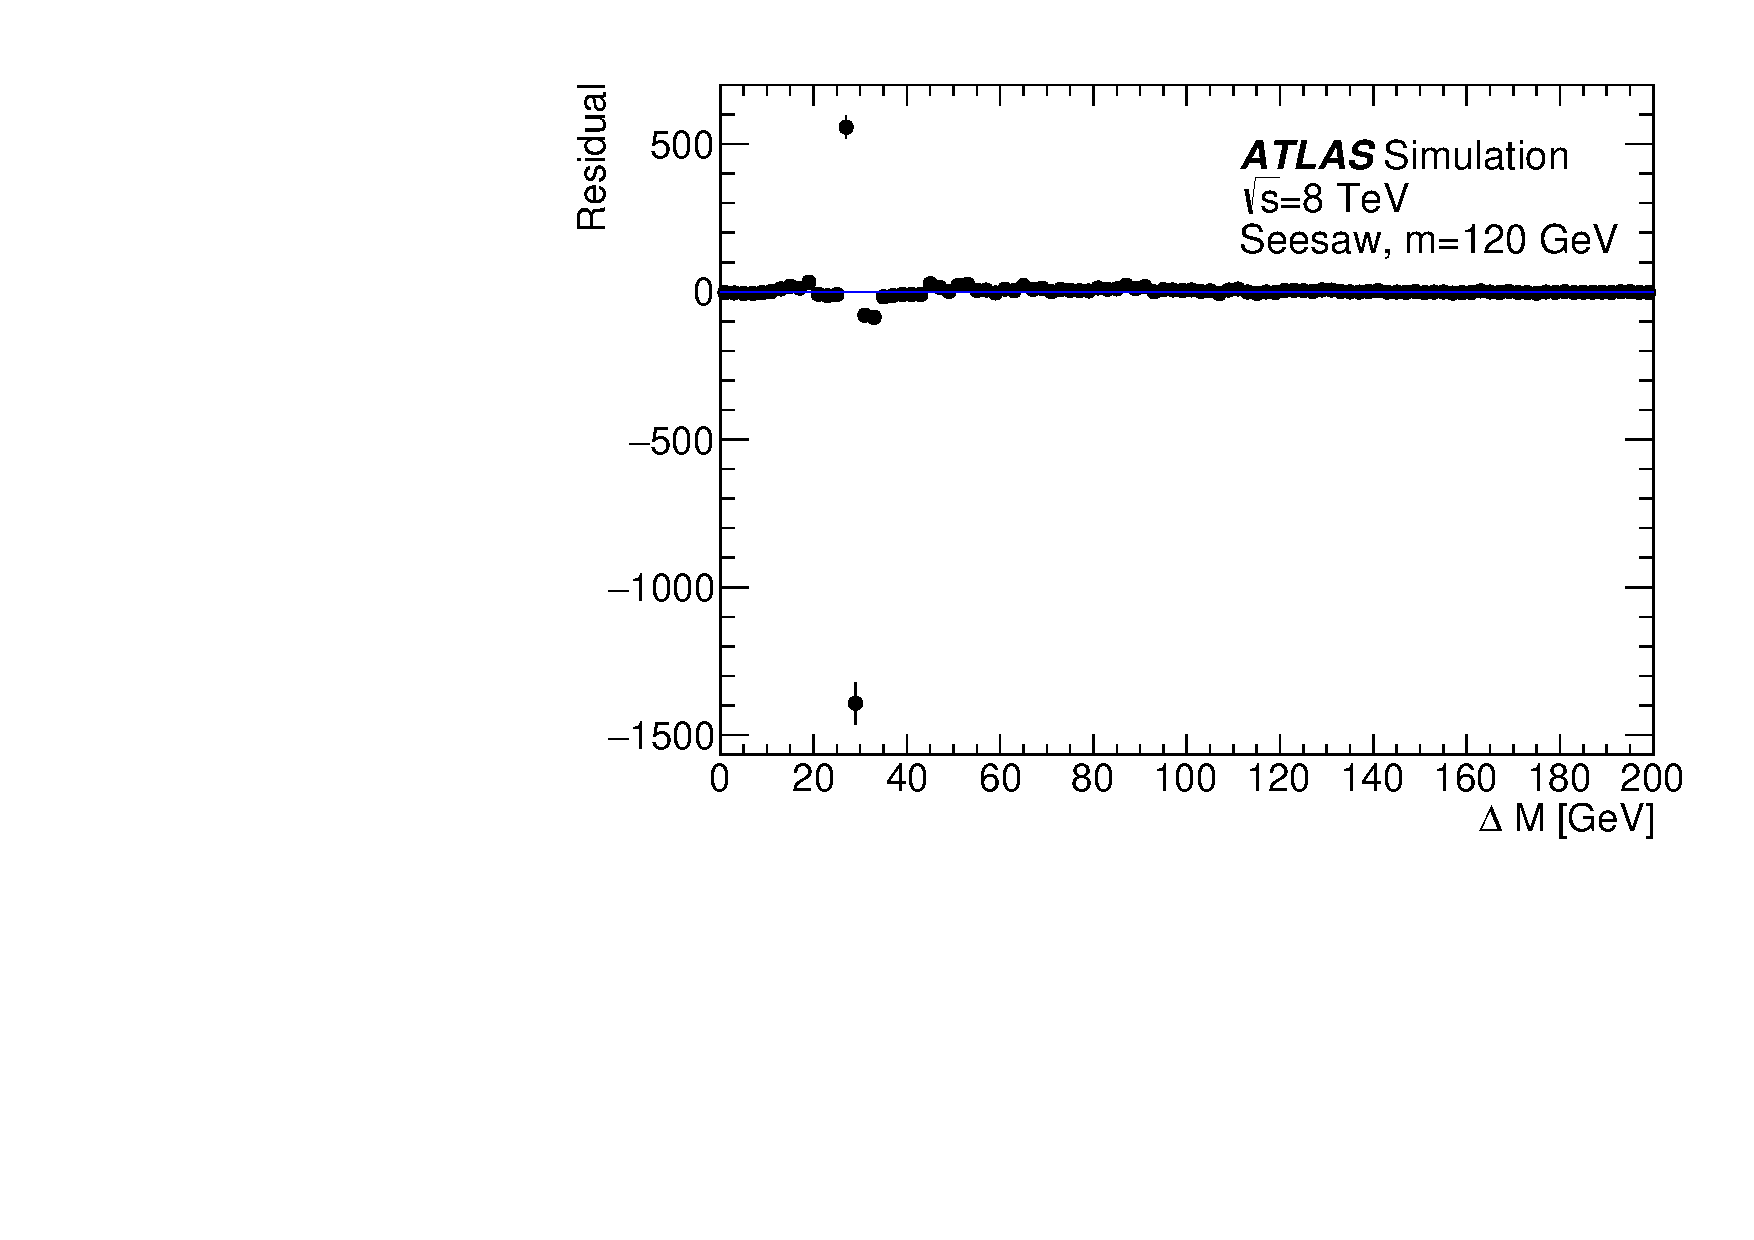
\includegraphics{figures/resonance/Seesaw_inclusive_sig120_Resid.pdf}}
	}
  \caption{Residuals of the simulated data with respect to the fit for $m_{3\ell}$ and $\deltam$ at the 120 GeV signal mass point. }
  \label{fig:Resid}
\end{minipage}
\label{fig:SigFit120}
\end{figure} 

The $\deltam$ distributions at each simulated mass point for both the type~III seesaw and the vector-like leptons models are fitted with the Voigtian plus Landau function, separately for each flavor channel and category. The fits for the $120 \GeV$ mass hypothesis of the type~III seesaw model are shown both for $\deltam$ and  $m_{3\ell}$, along with the corresponding pulls and residuals of the simulated data with respect to the fit, in figures~\ref{fig:SigFit}, \ref{fig:Pull}, and \ref{fig:Resid}. The same plots, but enlarged around the signal peak, are shown in figure~\ref{fig:fit-Sig_inclusive_zoom}. 

Tables~\ref{table:ZeFitParamsSS}, \ref{table:ZeFitParamsSS}, \ref{table:ZeFitParamsVLL}, and \ref{table:ZeFitParamsVLL} show the fitted parameters for the inclusive signal regions for each of the two flavor channels and signal models. As mentioned in section~\ref{sec:resonance-signal-mc-samples}, the type~III seesaw samples were simulated without intrinsic $Z$ width, and hence the width parameters vector-like leptons are used instead. Plots showing the fits to the $\deltam$ distributions are shown in appendix~\ref{sec:appendix-resonance-fitplots}.

Signal hypotheses at intermediate mass points between the simulated values are obtained by linearly interpolating the fit parameters determined at the nearest simulated points above and below. To validate the linear interpolation between the mass points, a closure test was performed comparing the fit parameters determined at a simulated mass point with the values obtained from a linear interpolation between the adjacent simulated points. The resulting fit for the $160 \GeV$ mass point is shown in Fig.~\ref{fig:sigclosure}. Further test and comparisons between the signal shapes of the two models are shown in appendix~\ref{appendix:signal-validation}.

\clearpage

\subsection{Background Fits}\label{sec:resonance-background-model}
The dominant diboson backgrounds are modeled using a Bukin function, a 5-parameter function designed to model asymmetric peaks:

\begin{equation}
\mathcal{P}(x;x_p ,\sigma_p, \xi ,\rho)=A_p \exp \left [ \frac{\xi \sqrt{\xi^2+1} (x-x_1) \sqrt{2\log2}}{\sigma_p(\sqrt{\xi^2+1}-\xi)^2 \log (\sqrt{\xi^2+1}+\xi)}+ \rho( \frac{x-x_i}{p_p-x_i})^2 - \log2\right ] ,
\end{equation}
where $\rho = \rho_1$ and $x = x_i$ for $x < x_1$, and $\rho = \rho_2$ and $x_i = x_2$ for $x \leq x_2$. The function describes the diboson $\deltam$ distribution well, in particular successfully modeling the turn-on region at low values of $\deltam$. However, the fit parameters are strongly correlated, with some pairs exceeding $99\%$ correlation. To reduce the number of free parameters, two parameters, $\sigma_p$ and $\xi_p$, are constrained to be linear functions of $x_p$ using pseudoexperiments. 100 toy datasets are generated from the fitted Bukin function, and the Bukin function fit is repeated on each dataset. The scatter plots of $\sigma_p$ versus $x_p$ and $\xi_p$ versus $x_p$ are shown in figure~\ref{fig:resonance-bukin-reduction}, along with the linear least squares fits used to constrain $\sigma_p$ and $\xi_p$. 

The results of the 3-parameter fits are shown with the decorrelated eigenvariations of the fit parameters in figures~\ref{fig:fit-results-Bukin3Par-WZ} and \ref{fig:fit-results-Bukin3Par-ZZ}. 

\begin{figure}[htbp]
    \centering
	\subfloat[ $WZ$, Inclusive, $\sigma_p$ vs $x_p$] {
		\resizebox{0.48\textwidth}{!}{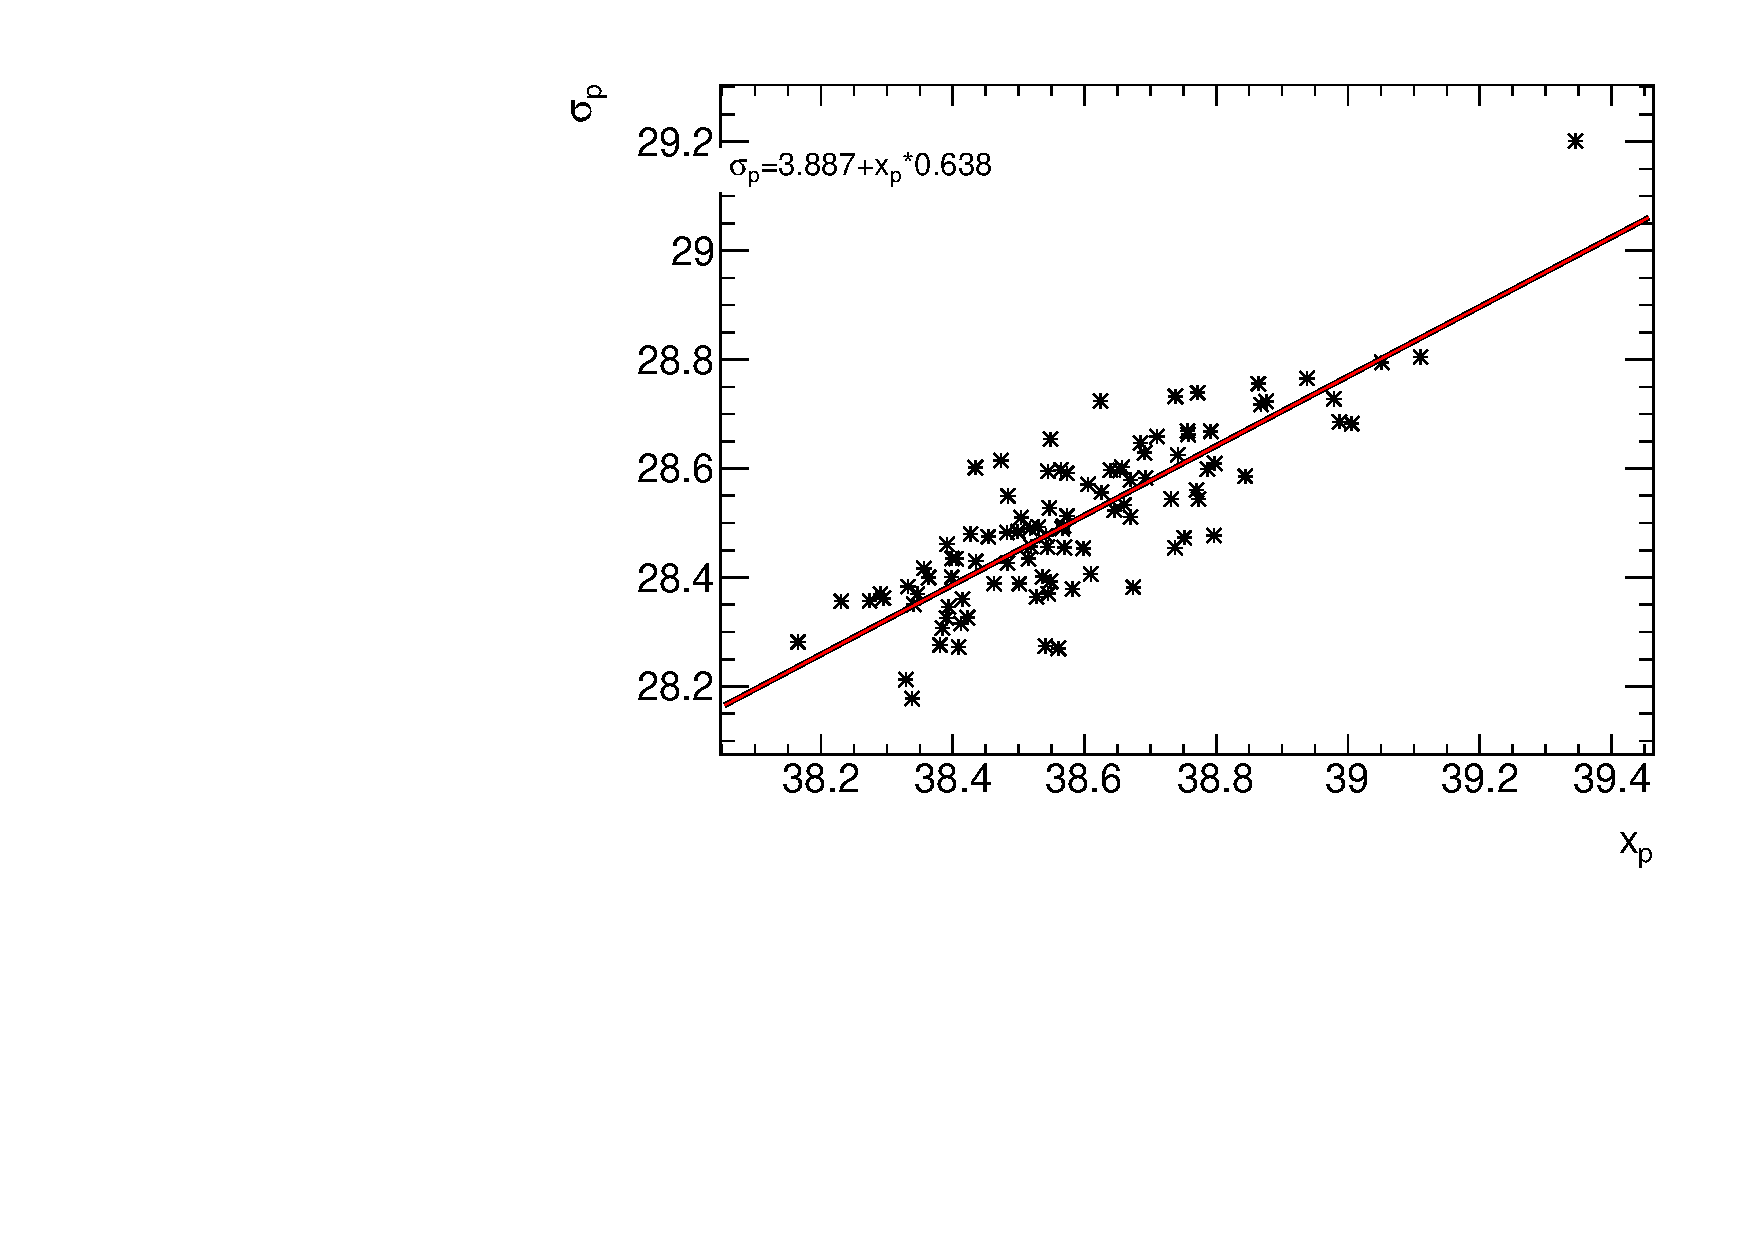
\includegraphics{figures/resonance/corr_fit_sigp_xp__WZ_hS.pdf}}
	}
	\subfloat[ $WZ$, Inclusive, $\xi_p$ vs $x_p$] {
			\resizebox{0.48\textwidth}{!}{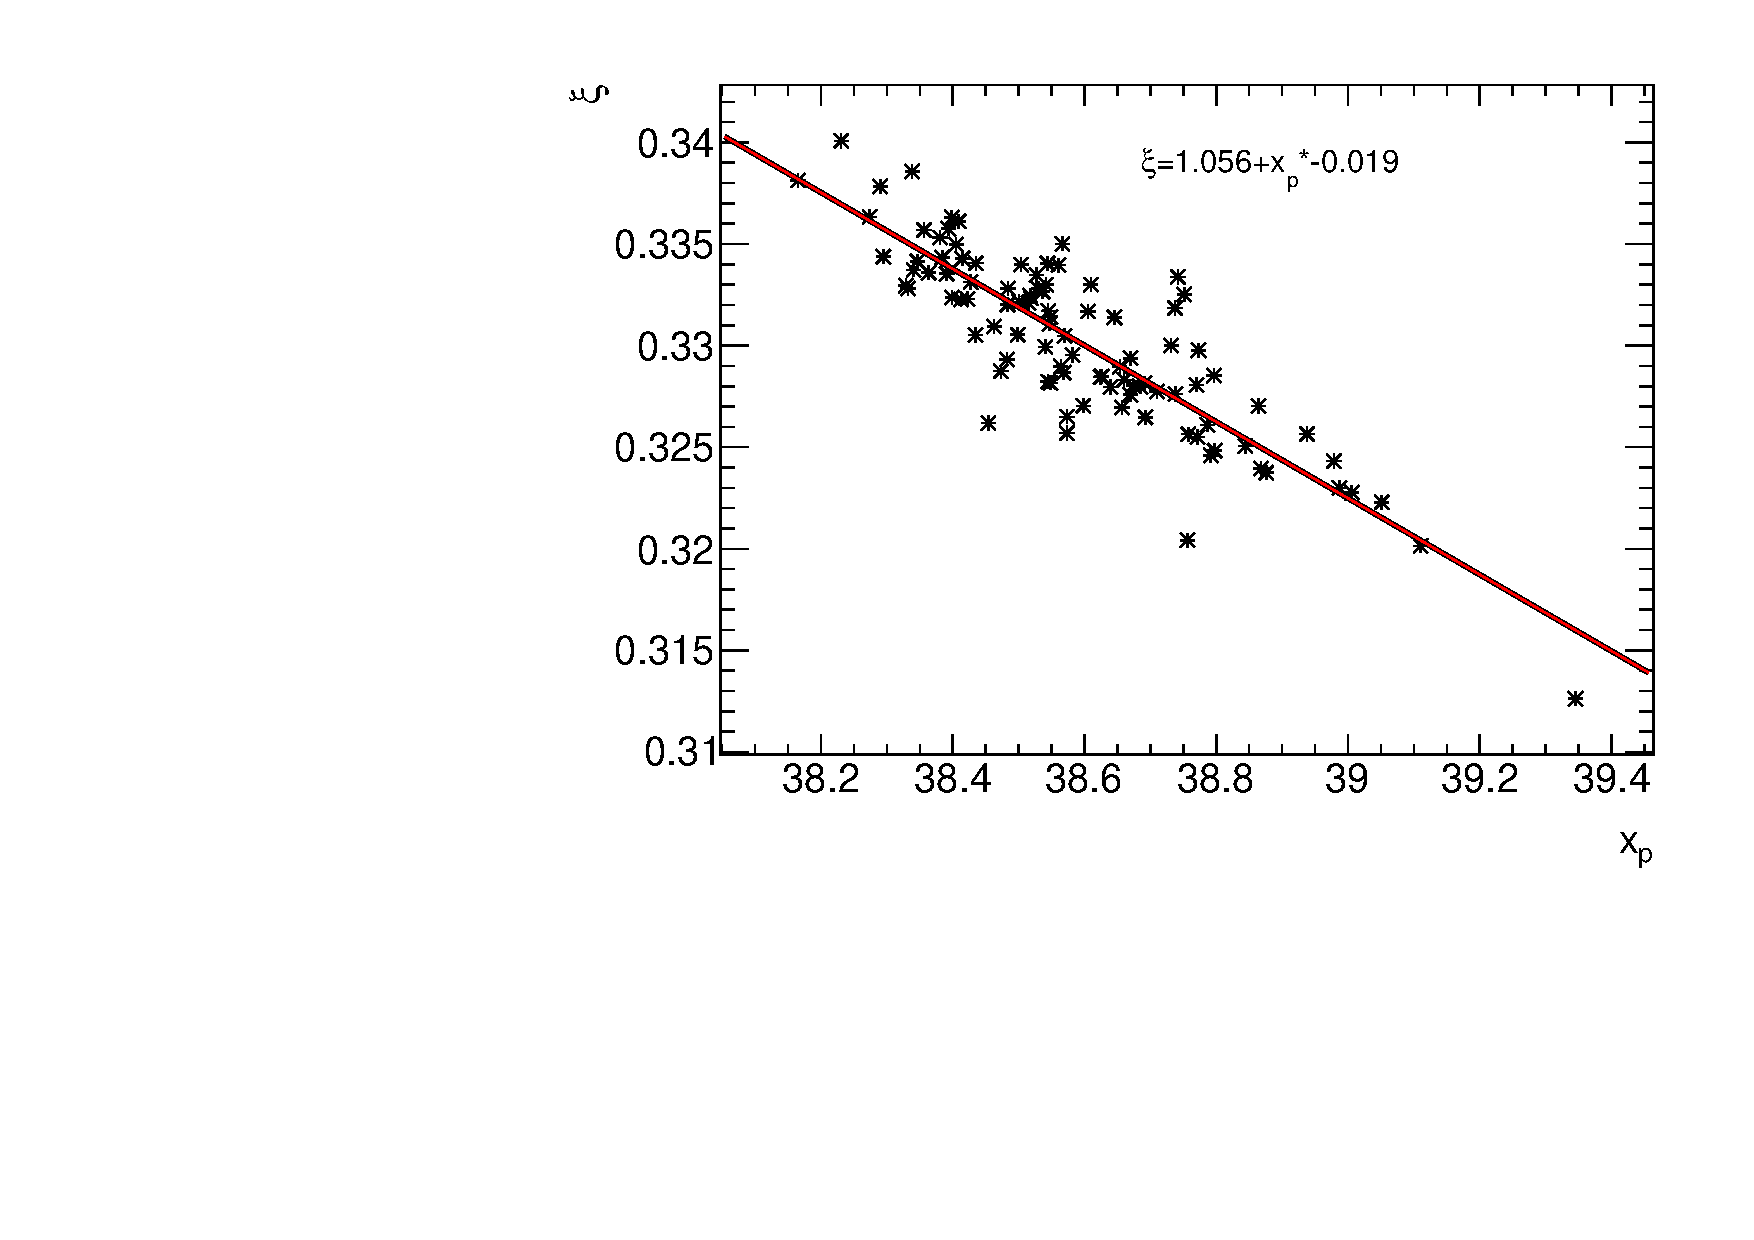
\includegraphics{figures/resonance/corr_fit_xi_xp__WZ_hS.pdf}}
         }
	\caption{Parameter correlation for 100 toy experiments, including the linear fit for the inclusive $WZ$ region. }
	\label{fig:CorrWZ}
\end{figure}

\begin{figure}[htbp]
    \centering
	\subfloat[ $ZZ$, Inclusive, $\sigma_p$ vs $x_p$] {
		\resizebox{0.48\textwidth}{!}{\includegraphics{figures/resonance/corr_fit_sigp_xp__ZZ_hS.pdf}}
	}
	\subfloat[ $ZZ$, Inclusive, $\xi_p$ vs $x_p$] {
			\resizebox{0.48\textwidth}{!}{\includegraphics{figures/resonance/corr_fit_xi_xp__ZZ_hS.pdf}}
         }
	\caption{Parameter correlation for 100 toy experiments, including the linear fit for the inclusive $ZZ$ region. }
	\label{fig:CorrZZ}
\end{figure}


\begin{figure}[htbp]
	\centering
	\subfloat[ Inclusive, $Z+e$] {
		\resizebox{0.48\textwidth}{!}{\includegraphics{figures/resonance/c_FitVariations_ZZ_Sherpa_Bukin3Par_InclusiveNoM3L_Ze_DeltaM_InclusiveNoM3L.pdf}}
	}
	\subfloat[ Inclusive, $Z+\mu$] {
		\resizebox{0.48\textwidth}{!}{\includegraphics{figures/resonance/c_FitVariations_ZZ_Sherpa_Bukin3Par_InclusiveNoM3L_Zmu_DeltaM_InclusiveNoM3L.pdf}}
	} \\
	\subfloat[ $\fourl$, $Z+e$] {
		\resizebox{0.48\textwidth}{!}{\includegraphics{figures/resonance/c_FitVariations_ZZ_Sherpa_Bukin3Par_FourLNoM3L_Ze_DeltaM_FourLNoM3L.pdf}}
	}
	\subfloat[ $\fourl$, $Z+\mu$] {
		\resizebox{0.48\textwidth}{!}{\includegraphics{figures/resonance/c_FitVariations_ZZ_Sherpa_Bukin3Par_FourLNoM3L_Zmu_DeltaM_FourLNoM3L.pdf}}
	} \\
	\subfloat[ $\threeljj$, $Z+e$] {
		\resizebox{0.48\textwidth}{!}{\includegraphics{figures/resonance/c_FitVariations_ZZ_Sherpa_Bukin3Par_ThreeLDijetNoM3L_Ze_DeltaM_ThreeLDijetNoM3L.pdf}}
	}
	\subfloat[ $\threeljj$, $Z+\mu$] {
		\resizebox{0.48\textwidth}{!}{\includegraphics{figures/resonance/c_FitVariations_ZZ_Sherpa_Bukin3Par_ThreeLDijetNoM3L_Zmu_DeltaM_ThreeLDijetNoM3L.pdf}}
	} \\
	\subfloat[ $\threelo$, $Z+e$] {
		\resizebox{0.48\textwidth}{!}{\includegraphics{figures/resonance/c_FitVariations_ZZ_Sherpa_Bukin3Par_ElseNoM3L_Ze_DeltaM_ElseNoM3L.pdf}}
	}
	\subfloat[ $\threelo$, $Z+\mu$] {
		\resizebox{0.48\textwidth}{!}{\includegraphics{figures/resonance/c_FitVariations_ZZ_Sherpa_Bukin3Par_ElseNoM3L_Zmu_DeltaM_ElseNoM3L.pdf}}
	} \\
	\caption{Restricted 3-parameter Bukin fits to the $ZZ$ $\deltam$ distributions in each signal region. The central value is shown in black, and the $1-\sigma$ eigenvariations of the fit parameters are shown in the colored dashed lines.}
	\label{fig:fit-results-Bukin3Par-ZZ}
\end{figure}

\begin{figure}[htbp]
	\centering
	\subfloat[ Inclusive, $Z+e$] {
		\resizebox{0.48\textwidth}{!}{\includegraphics{figures/resonance/c_FitVariations_WZ_Sherpa_Bukin3Par_InclusiveNoM3L_Ze_DeltaM_InclusiveNoM3L.pdf}}
	}
	\subfloat[ Inclusive, $Z+\mu$] {
		\resizebox{0.48\textwidth}{!}{\includegraphics{figures/resonance/c_FitVariations_WZ_Sherpa_Bukin3Par_InclusiveNoM3L_Zmu_DeltaM_InclusiveNoM3L.pdf}}
	} \\
	\subfloat[ $\threeljj$, $Z+e$] {
		\resizebox{0.48\textwidth}{!}{\includegraphics{figures/resonance/c_FitVariations_WZ_Sherpa_Bukin3Par_ThreeLDijetNoM3L_Ze_DeltaM_ThreeLDijetNoM3L.pdf}}
	}
	\subfloat[ $\threeljj$, $Z+\mu$] {
		\resizebox{0.48\textwidth}{!}{\includegraphics{figures/resonance/c_FitVariations_WZ_Sherpa_Bukin3Par_ThreeLDijetNoM3L_Zmu_DeltaM_ThreeLDijetNoM3L.pdf}}
	} \\
	\subfloat[ $\threelo$, $Z+e$] {
		\resizebox{0.48\textwidth}{!}{\includegraphics{figures/resonance/c_FitVariations_WZ_Sherpa_Bukin3Par_ElseNoM3L_Ze_DeltaM_ElseNoM3L.pdf}}
	}
	\subfloat[ $\threelo$, $Z+\mu$] {
		\resizebox{0.48\textwidth}{!}{\includegraphics{figures/resonance/c_FitVariations_WZ_Sherpa_Bukin3Par_ElseNoM3L_Zmu_DeltaM_ElseNoM3L.pdf}}
	} \\
	\caption{Restricted 3-parameter Bukin fits to the $WZ$ $\deltam$ distributions in each signal region. The central value is shown in black, and the $1-\sigma$ eigenvariations of the fit parameters are shown in the colored dashed lines.}
	\label{fig:fit-results-Bukin3Par-WZ}
\end{figure}



The shapes of the diboson $\deltam$ distributions in the categorized signal regions are compared to the inclusive signal regions using Kolmogorov-Smirnov tests, shown in figures~\ref{fig:inclusive-KS-tests-ZZ} and \ref{fig:inclusive-KS-tests-WZ} and tables~\ref{table:inclusive-KS-tests-ZZ} and \ref{table:inclusive-KS-tests-WZ}. The shapes of the $\deltam$ distributions in the $\fourl$ and $\threelo$ signal regions are consistent with the inclusive regions; therefore, to take advantage of the larger statistics in the inclusive signal region, \textbf{the shape from the inclusive signal region is used to model the $\fourl$ and $\threelo$ signal regions}. The final fits are shown in figures~\ref{fig:WZ-DiBosonFit} and \ref{fig:ZZ-DiBosonFit}.
 
\begin{figure}[htbp]
	\centering
	\subfloat[ $\fourl$ SR, $Z+e$] {
		\resizebox{2in}{!}{\includegraphics{figures/resonance/c_KSTests_ZZ_Sherpa_FourLNoM3L_Ze}}
	}
	\subfloat[ $\threeljj$ SR, $Z+e$] {
		\resizebox{2in}{!}{\includegraphics{figures/resonance/c_KSTests_ZZ_Sherpa_ThreeLDijetNoM3L_Ze}}
	}
	\subfloat[ $\threelo$ SR, $Z+e$] {
		\resizebox{2in}{!}{\includegraphics{figures/resonance/c_KSTests_ZZ_Sherpa_ElseNoM3L_Ze}}
	} \\
	\subfloat[ $\fourl$ SR, $Z+\mu$] {
		\resizebox{2in}{!}{\includegraphics{figures/resonance/c_KSTests_ZZ_Sherpa_FourLNoM3L_Zmu}}
	}
	\subfloat[ $\threeljj$ SR, $Z+\mu$] {
		\resizebox{2in}{!}{\includegraphics{figures/resonance/c_KSTests_ZZ_Sherpa_ThreeLDijetNoM3L_Zmu}}
	}
	\subfloat[ $\threelo$ SR, $Z+\mu$] {
		\resizebox{2in}{!}{\includegraphics{figures/resonance/c_KSTests_ZZ_Sherpa_ElseNoM3L_Zmu}}
	} \\
	\caption{Comparison of $ZZ$ $\deltam$ shapes between the inclusive signal region and the categorized signal regions, with empirical distribution functions.}
	\label{fig:inclusive-KS-tests-ZZ}
\end{figure}

\begin{table}[htbp]
	\centering
	\begin{tabular}{ccc}
		Signal Region & KS probability & $D$ \\
		\hline
		$\fourl$, $Z+e$ & 0.4109& 0.060 \\
		$\threeljj$, $Z+e$ & 0.001 & 0.122 \\
		$\threelo$, $Z+e$ & 0.782 & 0.019 \\
		$\fourl$, $Z+\mu$ & 0.520 & 0.043 \\
		$\threeljj$, $Z+\mu$ & 0.130 & 0.098 \\
		$\threelo$, $Z+\mu$ & 0.946 & 0.016
	\end{tabular}
	\caption{Results of KS tests comparing the $ZZ$ $\deltam$ shapes between the categorized signal regions and the inclusive signal regions.}
	\label{table:inclusive-KS-tests-ZZ}
\end{table}


\begin{figure}[htbp]
	\centering
	\subfloat[ $\threeljj$ SR, $Z+e$] {
		\resizebox{2in}{!}{\includegraphics{figures/resonance/c_KSTests_WZ_Sherpa_ThreeLDijetNoM3L_Ze}}
	}
	\subfloat[ $\threelo$ SR, $Z+e$] {
		\resizebox{2in}{!}{\includegraphics{figures/resonance/c_KSTests_WZ_Sherpa_ElseNoM3L_Ze}}
	} \\
	\subfloat[ $\threeljj$ SR, $Z+\mu$] {
		\resizebox{2in}{!}{\includegraphics{figures/resonance/c_KSTests_WZ_Sherpa_ThreeLDijetNoM3L_Zmu}}
	}
	\subfloat[ $\threelo$ SR, $Z+\mu$] {
		\resizebox{2in}{!}{\includegraphics{figures/resonance/c_KSTests_WZ_Sherpa_ElseNoM3L_Zmu}}
	} \\
	\caption{Comparison of $WZ$ $\deltam$ shapes between the inclusive signal region and the categorized signal regions, with empirical distribution functions. The $\fourl$ signal regions are not shown due to the lack of $WZ$ events with four leptons.}
	\label{fig:inclusive-KS-tests-WZ}
\end{figure}

 \begin{table}[htbp]
	\centering
	\begin{tabular}{ccc}
		Signal Region & KS probability & $D$ \\
		\hline
		$\threeljj$, $Z+e$ & 0.0 & 0.165 \\
		$\threelo$, $Z+e$ & 0.012 & 0.016 \\
		$\threeljj$, $Z+\mu$ & 0.0 & 0.152 \\
		$\threelo$, $Z+\mu$ & 0.0349 & 0.012
	\end{tabular}
	\caption{Results of KS tests comparing the $WZ$ $\deltam$ shapes between the categorized signal regions and the inclusive signal regions.}
	\label{table:inclusive-KS-tests-WZ}
\end{table}

\begin{figure}[htbp]
    \centering
	\subfloat[ $WZ$, Inclusive, $\deltam$] {
		\resizebox{0.48\textwidth}{!}{\includegraphics{figures/resonance/fit_WZ_hS.pdf}}
	}
	\subfloat[ $WZ$, Dijet, $\deltam$] {
			\resizebox{0.48\textwidth}{!}{\includegraphics{figures/resonance/fit_WZ_3Ljj_hS.pdf}}
         }
	\caption{$\deltam$ distributions for $WZ$ and Bukin function fits for the inclusive and the $\threeljj$ signal regions. The separate fits for the $Z+e$ and $Z+\mu$ flavor channels can be found in Appendix~\ref{sec:appendix-fitplots}.}
	\label{fig:WZ-DiBosonFit}
\end{figure}
 
 
\begin{figure}[htbp]
    \centering
	\subfloat[ ZZ, Inclusive, $\deltam$] {
		\resizebox{0.48\textwidth}{!}{\includegraphics{figures/resonance/fit_ZZ_hS.pdf}}
	}
	\subfloat[ ZZ,Dijet,  $\deltam$] {
			\resizebox{0.48\textwidth}{!}{\includegraphics{figures/resonance/fit_ZZ_3Ljj_hS.pdf}}
         }
	\caption{Final $\deltam$ distributions for $ZZ$ and Bukin function fits for the inclusive and the $\threeljj$ signal regions. The separate flavour fits can be found in Appendix~\ref{sec:appendix-fitplots}.}
	\label{fig:ZZ-DiBosonFit}
\end{figure}



The most important remaining backgrounds are due to reducible processes and $Z(ll)+\gamma$. The $Z(ll)+\gamma$ background is only significant in the $Z+e$ signal regions. Due to the limited statistics from the fake factor estimate, the individual categories are combined into a single inclusive distribution for electron and muons. The reducible backgrounds are fitted with Landau distributions, shown in figure~\ref{fig:reducible-landau-fits}. The individual regions are then normalized to the expectations from the individual categories~\footnote{In categories where the fake factor method predicts overall normalization that is negative but consistent with zero within statistical uncertainties, which can occur due to the prompt subtraction, the normalization is set to zero.}.

 The $Z(ll)+\gamma$ background is only significant in the $\threelo$, $Z+e$ signal region. This background is modeled with the sum of a Landau and a Gaussian, shown in figure~\ref{fig:eegamma}. The remaining small contributions from $\ttbarV$ and triboson processes are modeled together with a Landau function, shown in figure~\ref{fig:ttV}. 


\begin{figure}[htbp]
    \centering
	\subfloat[ Reducible bachelor electron, $\deltam$ ] {
		\resizebox{0.48\textwidth}{!}{\includegraphics{figures/resonance/fit_reducible_Ze.pdf}}
	}                                                                                                    
	\subfloat[ Reducible bachelor muon, $\deltam$ ] {
		\resizebox{0.48\textwidth}{!}{\includegraphics{figures/resonance/fit_reducible_Zmu.pdf}}
	}                                                                                                      
	\caption{The shape of the reducible background is taken from the estimates from the fake factor method. The distribution is parametrized with a Landau for both bachelor lepton flavors. Due to the limited statistics in the categorized signal regions, the shape is determined in the inclusive signal region, and only the normalization varies in the categorized signal regions.}
	\label{fig:reducible-landau-fits}
\end{figure}


\begin{figure}[htbp]
\centering
   \includegraphics[width=0.6\textwidth]{figures/resonance/fit_llgamma_Ze.pdf}
  \caption{The $\deltam$ distribution for the $Z+\gamma$ background, fitted with the sum of a Landau and a Gaussian. This background is significant for final states with a bachelor electron.} 
  \label{fig:eegamma}
\end{figure} 


\begin{figure}[htbp]
\centering
   \includegraphics[width=0.6\textwidth]{figures/resonance/fit_ttV_VVV.pdf}
  \caption{The $\deltam$ distribution for the combined  $t\overline{t}+V$, $VVV^{(*)}$  background, fitted with the sum of a Landau and a Gaussian. This background is significant for final states with a bachelor electron.} 
  \label{fig:ttV}
\end{figure} 


\clearpage


\section{Results}\label{sec:resonance-results}

The total number of observed events each signal region is shown in table~\ref{table:SR-event-counts}. The predicted backgrounds before and after performing the unbinned maximum-likelihood fit in the background-only hypothesis are also shown. The $\deltam$ distributions for the pre-fit background estimates and the data are shown in figure~\ref{fig:SR-DeltaM}, with examples signals from the vector-like leptons model with $m_{\lpm}=140 \GeV$ and the type~III seesaw model with $m_{\lpm}=300 \GeV$ also shown. The data agree with the background expectation in all cases, and no clear peak indicating resonant trilepton production is seen in any of the signal regions. 

\begin{figure}[htbp]
  \centering
  \subfloat[] {% [$Z+e$, $\fourl$ category] {
    \includegraphics[width=0.4\columnwidth]{figures/resonance/c_output_DeltaM_Ze_FourLNoM3L_300GeV_hide_ratio.pdf}
  }
  \subfloat[] {% [$Z+\mu$, $\fourl$ category] {
    \includegraphics[width=0.4\columnwidth]{figures/resonance/c_output_DeltaM_Zmu_FourLNoM3L_300GeV_hide_ratio.pdf}
  } \\
  \subfloat[] {% [$Z+e$, $\threeljj$ category] {
    \includegraphics[width=0.4\columnwidth]{figures/resonance/c_output_DeltaM_Ze_ThreeLDijetNoM3L_300GeV_hide_ratio.pdf}
  }
  \subfloat[] {% [$Z+\mu$, $\threeljj$ category] {
    \includegraphics[width=0.4\columnwidth]{figures/resonance/c_output_DeltaM_Zmu_ThreeLDijetNoM3L_300GeV_hide_ratio.pdf}
  } \\
  \subfloat[] {% [$Z+e$, $\threelo$ category] {
    \includegraphics[width=0.4\columnwidth]{figures/resonance/c_output_DeltaM_Ze_ElseNoM3L_300GeV_log.pdf}
  }
  \subfloat[] {% [$Z+\mu$, $\threelo$ category] {
    \includegraphics[width=0.4\columnwidth]{figures/resonance/c_output_DeltaM_Zmu_ElseNoM3L_300GeV_log.pdf}
  }
   \caption{The $\deltam = m_{3\ell}-m_{\ell^+\ell^-}$ distributions for the $\fourl$ (top), $\threeljj$ (middle), and $\threelo$ (bottom) categories, divided into the $Z+e$ (left) and $Z+\mu$ (right) flavour channels. The observed data are shown as black points, while the pre-fit background expectations are shown in the coloured histograms. Also shown are examples for signal contributions for a 140~GeV $\lpm$ in the vector-like leptons model and a 300~GeV $\lpm$ in the type~III seesaw model. The error bars on the data points represent statistical uncertainties, and the shaded bands represent the systematic uncertainties on the background predictions.}
  \label{fig:SR-DeltaM}
\end{figure}

\begin{table}[h]
	\renewcommand{\arraystretch}{1.5}
	\centering
	\caption{Observed and expected number of events in the six signal regions, before and after the combined unbinned maximum-likelihood fit. The pre-fit uncertainties represent the total systematic uncertainties on the background estimates. The post-fit uncertainties are determined by the maximum-likelihood fit.}
	\sisetup{ table-number-alignment=center,
	separate-uncertainty=true,
	%   table-figures-integer = 1,
	%table-figures-decimal = 2
	}
	\footnotesize
	\begin{tabular}{ | c ||
	S[separate-uncertainty,table-figures-uncertainty=1] |
	S[separate-uncertainty ,table-figures-uncertainty=1]|
	S[separate-uncertainty,table-figures-uncertainty=1] ||
	S[separate-uncertainty,table-figures-uncertainty=1] |
	S[separate-uncertainty,table-figures-uncertainty=1] |
	S[separate-uncertainty,table-figures-uncertainty=1] |
	%             S[separate-uncertainty,table-figures-uncertainty=1] |
	}
		\hline
		&	\multicolumn{3}{c||}{$Z+e$}	&	\multicolumn{3}{c|}{$Z+\mu$}	\\
		\hline
		Process	&	{$4$l SR}	&	{$3l+jj$ SR}	&	{$3l$-only SR}	 &	{$4l$ SR}	&	{$3l+jj$ SR}	&	{$3l$-only SR}	\\
		\hline
		\hline
		& \multicolumn{6}{c|}{Before combined background-only fit} \\
		\hline

		$ZZ$	&	10.9 \pm 0.6	&	11.7 \pm 0.8	&	91 \pm 5	&	21.4 \pm 1.1	&	7.5 \pm 0.6	&	90 \pm 5	\\
		\hline
		$WZ$	&	0.08 \pm 0.01	&	35.3 \pm 3.1	&	337 \pm 28	 &  {\textemdash}	 & 	46 \pm 4	 & 	480 \pm 40	\\
		\hline
		$Z+\gamma$	&   {\textemdash}	 & 	2.3 \pm 0.8	 & 	35 \pm 11	 & 	  {\textemdash}	 & 	  {\textemdash}	 & 	{\textemdash}	\\
		\hline
		Reducible	 & 	  {\textemdash}	 & 	1.6 \pm 0.5	 & 	38 \pm 14	 & 	1.5 \pm 0.3	 & 	8.8 \pm 3.0	 & 	79 \pm 22	\\
		\hline
		$t\overline{t}+V, VVV^{(*)} $ &  1.2 \pm 0.2  &  7.8 \pm 1.7  &  2.3 \pm 0.4  &  1.5 \pm 0.2  &  9.5 \pm 2.1  &  3.3 \pm 0.5 \\
		\hline
		Total Background & 	12.2 \pm 0.7	 & 	59 \pm 4	 & 	504 \pm 34	 & 	24.4 \pm 1.2	 & 	72 \pm 6	 & 	650 \pm 50 	\\
		\hline
		\hline
		& \multicolumn{6}{c|}{After combined background-only fit} \\
		\hline
		$ZZ$ & 15 \pm 4 &   13.4\pm 2.3 &  107\pm 9 & 22 \pm 5 &  10.1 \pm 1.6 &  88 \pm 8 \\
		\hline
		$WZ$ & 0.08 \pm 0.03 &   39 \pm 6 &  393 \pm 28 & 0.02 \pm 0.02 &   56 \pm 9 &  460 \pm 40 \\
		\hline
		$Z + \gamma$ &   {\textemdash} &   2.2 \pm 0.8 &  34 \pm 11 &   {\textemdash} &    {\textemdash} &   {\textemdash} \\
		\hline
		Reducible &   {\textemdash}  &   1.8 \pm 1.2 &  37 \pm 13 & 1.8 \pm 0.9 &  10.2 \pm 2.8 &  92 \pm 24 \\
		\hline
		$t\overline{t}+V, VVV^{(*)}$  & 1.1\pm 0.3 &   7.5 \pm 1.7 &  2.5 \pm 0.6 & 1.5\pm 0.4 &  9.1 \pm 2.1 &  3.3 \pm 0.8 \\
		\hline
		Total Background & 16 \pm 4 & 64\pm7  & 574\pm 34 &  25\pm5  & 85\pm10 &  640\pm40 \\
		\hline
		\hline
		Data 	&	\multicolumn{1}{c|}{16}	&	\multicolumn{1}{c|}{64}	&	\multicolumn{1}{c||}{573}	&	\multicolumn{1}{c|}{25}	&	\multicolumn{1}{c|}{86}	&	\multicolumn{1}{c|}{651}	\\
		\hline
	\end{tabular} 

	%		\hline
	%			&\multicolumn{3}{c||}{$Z+e$}	&	\multicolumn{3}{c|}{$Z+\mu$}	\\
	%		\hline
	%		Process	&	$4l$ SR	&	$3l+jj$ SR	&	$3l$-only SR	&	$4l$ SR	&	$3l+jj$ SR	&	$3l$-only SR	\\
	%		\hline
	%    \hline
	%     & \multicolumn{6}{c|}{Pre-Fit} \\
	%    \hline
	%
	%		$ZZ$	&	$10.9 \pm 0.6$	&	$11.7 \pm 0.8$	&	$91.3 \pm 5.0$	&	$21.4 \pm 1.1$	&	$7.5 \pm 0.6$	&	$90.4 \pm 4.8$	\\
	%		\hline
	%		$WZ$	&	$0.08 \pm 0.01$	&	$35.3 \pm 3.1$	&	$337 \pm 28$	&	$-$	&	$46.3 \pm 4.2$	&	$475 \pm 39$	\\
	%		\hline
	%		$Z+\gamma$	&	$-$	&	$2.3 \pm 0.8$	&	$35 \pm 11$	&	$-$	&	$-$	&	$-$	\\
	%		\hline
	%		Reducible	&	$-$	&	$1.6 \pm 0.5$	&	$38 \pm 14$	&	$1.5 \pm 0.3$	&	$8.8 \pm 3.0$	&	$79 \pm 22$	\\
	%		\hline
	%    $t\overline{t}+V$, $VVV^{(*)}$ & $1.2 \pm 0.2$ & $7.8 \pm 1.7$ & $2.3 \pm 0.4$ & $1.5 \pm 0.2$ & $9.5 \pm 2.1$ & $3.3 \pm 0.5$ \\
	%		\hline
	%		Total Background	&	$12.2 \pm 0.7$	&	$58.7 \pm 4.1$	&	$504 \pm 34$	&	$24.4 \pm 1.2$	&	$72.1 \pm 5.9$	&	$647 \pm 46$	\\
	%		\hline
	%		\hline
	%     & \multicolumn{6}{c|}{Post-Fit} \\
	%    \hline
	%    ZZ & $14.9 \pm 4.1$ & $  13.4\pm 2.3$ & $ 106.5 \pm 8.8$ & $21.8 \pm 5.1$ & $ 10.1 \pm 1.6$ & $ 88.0 \pm 7.7$ \\
	%    \hline
	%    WZ & $0.08 \pm 0.03$ & $  39.1 \pm 6.4$ & $ 393.0 \pm 27.9$ & $0.02 \pm 0.02$ & $  56.0 \pm 8.7$ & $ 460.9 \pm 35.5$ \\
	%    \hline
	%    $Z + \gamma$ & $-$ & $  2.2 \pm 0.8$ & $ 34.2 \pm 10.8$ & $ -$ & $  -$ & $ - $ \\
	%    \hline
	%    Reducible & $-$ & $  1.8 \pm 1.2$ & $ 37.4 \pm 12.6$ & $1.8 \pm 0.9$ & $ 10.2 \pm 2.8$ & $ 92.1 \pm 23.9$ \\
	%    \hline
	%    $t\overline{t}+V$, $VVV^{(*)}$  & $1.1\pm 0.3$ & $  7.5 \pm 1.7$ & $ 2.5 \pm 0.6$ & $1.5\pm 0.4$ & $ 9.1 \pm 2.1$ & $ 3.3 \pm 0.8$ \\
	%    \hline
	%    Total Background & $16.1 \pm 4.1$ & $64.0\pm7.2$  & $573.6 \pm 33.6$ &  $25.1\pm5.2$  & $85.4\pm9.5$ &  $644.3\pm43.5$ \\
	%    \hline
	%    \hline
	%		Data&	$16$	&	$64$	&	$573$	&	$25$	&	$86$	&	$651$	\\
	%		\hline
	%	\end{tabular}
	%
	\label{table:SR-event-counts}
\end{table}

\begin{figure}[htbp]
  \centering	
  \subfloat[ ] {%Background only fit,  $Z+e$] {
    \resizebox{0.48\textwidth}{!}{\includegraphics{figures/resonance/Fit_BGOnly_Ze_ErrorBand.pdf}}
  }
  \subfloat[ ] {%Background only fit, $Z+\mu$] {
    \resizebox{0.48\textwidth}{!}{\includegraphics{figures/resonance/Fit_BGOnly_Zmu_ErrorBand.pdf}}
  } \\
  \caption{Projections onto the $\deltam$ variable of the background-only unbinned maximum-likelihood fits, shown superimposed on the data with the three categories in each flavour channel added together. The $Z+e$ flavour channel is shown in (a), and the $Z+\mu$ channel is shown in (b). The contributions of the separate background components to the total background-only fit are also shown. The error bars on the data points represent statistical uncertainties. Good agreement is observed between the background model and the data.}
  \label{fig:FitResult}
\end{figure}

Good agreement is seen between the pre-fit and post-fit normalizations for the $\fourl$ and $\threeljj$ categories in the $Z+\mu$ flavour channel. The largest change in normalization due to the fit is in the $\fourl$ category for the $Z+e$ flavour channel, where the fitted $ZZ$ normalization exceeds the prediction by $35\%$. The $WZ$ and $ZZ$ normalizations increase by roughly $15\%$ in the $\threeljj$ and $\threelo$ categories in the $Z+e$ flavour channel, and $30\%$ in the $\threeljj$ category in the $Z+\mu$ flavour channel. The projections of the fit results in the background-only hypothesis are shown in figure~\ref{fig:FitResult} for the combination of the three categories in each flavour channel.




\section{Interpretation}\label{sec:resonance-interpretation}
The data are well described by the combined fit to the three categories in each flavour channel. The consistency of the data with the background-only hypothesis is evaluated by scanning the local $p_0$-value for the $\deltam$ distribution in $3 \GeV$ intervals for signal mass hypotheses in the range $100-400 \GeV$ for the vector-like leptons model, and $100-500 \GeV$ for the seesaw model, using the unbinned maximum-likelihood fit described in section~\ref{sec:resonance-fit-method} with the signal strength set to zero. The agreement is expressed in terms of the $p_0$-value, the probability that, assuming the background-only hypothesis is true, an experiment would yield at least as many events as observed in the current measurement. The $p_0$ values are calculated using the frequentist hypothesis test based on the profile likelihood ratio test statistic and approximated with asymptotic formulae~\cite{asimov}. The minimum $p_0$-value is $p_0=0.02$ at a mass of $183~\GeV$ for the $Z+e$ flavour channel, and $p_0=0.05$ at a mass of $109~\GeV$ for the $Z+\mu$ flavour channel.

\subsection{Limits on Models}

Since no significant excess above the background expectation is observed, the fit model is used to derive 95\% confidence level (CL) exclusion limits on the heavy lepton pair-production cross section, $\sigma$, using the $CL_s$ method~\cite{CLs}. The limits are shown for the vector-like leptons model in figure~\ref{fig:VLLLimit}, and for the type~III seesaw model in figure~\ref{fig:T3SSLimit}, evaluated in the same $3 \GeV$ intervals as the $p_0$-values.
The vector-like leptons model is excluded for electron-only mixing in the heavy lepton mass ranges $129$--$144 \GeV$ and $163$--$176 \GeV$, with an expected exclusion in the range $109$--$152 \GeV$. The corresponding observed (expected) exclusion for the muon-only mixing scenario is $114$--$153 \GeV$ and $160$--$168 \GeV$ ($105$--$167 \GeV $).
The significantly higher production cross sections for the type~III seesaw model lead to an observed (expected) exclusion in the electron-only mixing scenario in the heavy lepton mass range $100$--$430 \GeV$  ($100$--$436 \GeV$). For the muon-only mixing scenario, the observed exclusion is in the ranges $100$--$401 \GeV$ and $419$--$468 \GeV$, while the expected exclusion is $100$--$419 \GeV$.

\begin{figure}[htbp]
  \centering	
  \subfloat[] {
    \resizebox{0.5\textwidth}{!}{\includegraphics{figures/resonance/LimitVLL_Ze_NP.pdf}}
  }
  \subfloat[] {
    \resizebox{0.5\textwidth}{!}{\includegraphics{figures/resonance/LimitVLL_Zmu_NP.pdf}}
  } \\
  \caption{$95 \%$ CL upper limits on the vector-like lepton cross section. The left (right) plot shows the limits assuming $100\%$ branching fraction to $e/\nu_e$ ($\mu/\nu_{\mu}$). The solid line shows the observed limit. The dashed line shows the median expected limit for a background-only hypothesis, with green and yellow bands indicating the expected fluctuations at the $\pm1\sigma$ and $\pm 2 \sigma$ levels. The limit is evaluated in $3 \GeV$ intervals.}
  \label{fig:VLLLimit}
\end{figure}

\begin{figure}[htbp]
  \centering
  \subfloat[] {
     \resizebox{0.5\textwidth}{!}{\includegraphics{figures/resonance/SeesawZe_ShapeInterpol_xsectot_plot}}
  }
  \subfloat[] {
     \resizebox{0.5\textwidth}{!}{\includegraphics{figures/resonance/SeesawZmu_ShapeInterpol_xsectot_plot}}
  }
  \caption{$95 \%$ CL upper limits on the type~III seesaw production cross section. The left (right) plot shows the limits assuming $100\%$ branching fraction to $e/\nu_e$ ($\mu/\nu_{\mu}$). The solid line shows the observed limit. The dashed line shows the median expected limit for a background-only hypothesis dataset, with green and yellow bands indicating the expected fluctuations at the $\pm1\sigma$ and $\pm 2 \sigma$ levels. The limit is evaluated in $3 \GeV$ intervals.}
  \label{fig:T3SSLimit}
\end{figure}

\subsubsection{Model-Independent Limits}

The constraints shown in figures~\ref{fig:VLLLimit} and \ref{fig:T3SSLimit} are relevant to the specific VLL and type~III seesaw models considered, and are not necessarily applicable to other scenarios predicting trilepton resonances with an intermediate $Z$ boson. A more model-independent observable is the \emph{visible cross section}, $\sigmavis$, defined as the number of observed events with $Z+\ell$-induced trilepton resonances for a given resonance mass divided by the integrated luminosity of the data sample, 20.3~\ifb. The 95\% CL upper limits on $\sigmavis$, denoted $\sigma_{95}^{\mathrm{vis}}$, are derived from a fit to each flavour channel with $f_V=1$, i.e. using only the peak component of the signal. The results for the two flavour channels, derived from the inclusive event selection without dividing the events into the three categories, are shown in figure~\ref{fig:N95}.

The limits on $\sigmavis$ can be used to test specific models after taking into account the model's acceptance with respect to a fiducial volume, $\mathcal{A}$, and reconstruction and selection efficiency of events within the fiducial volume, $\epsilon_{\mathrm{fid}}$. The 95\% CL upper limit on the cross section for the model is given by:

\begin{equation}\label{eqn:sigma95}
	\sigma_{95} = \frac{\sigma_{95}^{\mathrm{vis}}}{\mathcal{A}\times \epsilon_{\mathrm{fid}}}.
\end{equation}

The acceptance $\mathcal{A}$ is defined as the probability for generated signal events to lie within a fiducial volume defined by the kinematics of the generated leptons. The leptons are considered at \emph{particle level}, i.e. after parton shower and hadronization and with lifetimes longer than $10^{-11}$~s, and are \emph{dressed}, including the contributions from radiated photons within a cone of $\Delta R=0.1$. The fiducial volume requires that events contain an $\lpm$ decaying to a prompt electron or muon and a $Z$ boson that then decays to electrons or muons. The three leptons from the $\lpm$ decay are required to have $\pt>15~\GeV$ and lie within $|\eta|<2.5$, with at least one lepton satisfying $\pt>26~\GeV$. Two of the leptons must form a same-flavour opposite-sign pair with a mass within $10 \GeV$ of $m_Z$, and the $Z$ boson and the off-$Z$ lepton must be separated by $\Delta R < 3$.  The events are divided into flavour channels according to the flavour of the off-$Z$ lepton. For the VLL and type~III seesaw models used in this analysis, the acceptance of events containing an $\lpm\rightarrow Z(\ell\ell)\ell$ decay to fall within the fiducial volume is in the range $60\%$--$65\%$ for most of the mass range, decreasing at higher masses due to the cut on the $\Delta R$ between the $Z$ boson and the off-$Z$ lepton. The acceptance decreases at low masses due to the lepton $\pt$ requirement, reaching $30\%$--$35\%$ at $m_{\lpm}=100 \GeV$.

For type~III seesaw and VLL events within the fiducial volume, $\epsilon_{\mathrm{fid}}$ ranges from 20\% to 49\% if the other heavy lepton decays to a neutrino and a $W$, $Z$, or $H$ boson. If the other heavy lepton decays to an electron or a muon, the efficiency is 10\%--20\% lower, due to the increased probability of incorrectly selecting the off-$Z$ lepton. The event selection efficiencies for the type~III seesaw model in scenarios where the second heavy lepton decays to a $W$ boson are shown in figure~\ref{fig:fiducial-efficiencies-inclusive} as a function of $m_{\lpm}$; the efficiencies for scenarios where the second heavy lepton decays to a $Z$ or $H$ boson and for the vector-like leptons model are consistent with these efficiencies within the statistical uncertainties.


\begin{figure}[htbp]
  \subfloat[] {%[$Z+e$]{
  	\includegraphics[width=0.48\columnwidth]{figures/resonance/SeesawZe_N95_Inclusive}
  }
  \subfloat[] {%[$Z+\mu$]{
  	\includegraphics[width=0.48\columnwidth]{figures/resonance/SeesawZmu_N95_Inclusive}
  }
  \caption{Upper limits at 95\% CL on $\sigmavis$ for the $Z+e$ (left) and $Z+\mu$ (right) flavour channels, derived without dividing events into the three categories. The limits are evaluated in $3 \GeV$ intervals.}
  \label{fig:N95}
\end{figure}

\begin{figure}[htbp]
  \subfloat[] {%[$Z+e$]{
  	\includegraphics[width=0.48\columnwidth]{figures/resonance/c_fid_eff_vs_mass_Ze_InclusiveNoM3L_Seesaw_minimal}
  }
  \subfloat[] {%[$Z+\mu$]{
  	\includegraphics[width=0.48\columnwidth]{figures/resonance/c_fid_eff_vs_mass_Zmu_InclusiveNoM3L_Seesaw_minimal}
  }
  \caption{Efficiencies for reconstructing and correctly identifying the $\lpm\rightarrow Z(\ell\ell)\ell^{\pm}$ decay in events within the fiducial volume for the type~III seesaw model. The left (right) plot shows the efficiencies for events containing a $\lpm\rightarrow Z(\ell\ell)e$ ($\lpm\rightarrow Z(\ell\ell)\mu$) decay. The decay of the second heavy lepton is specified in the legend. The shaded bands show the statistical uncertainty.}
  \label{fig:fiducial-efficiencies-inclusive}
\end{figure}

\printbibliography